\documentclass[twoside,english,a4paper,12pt]{uiofysmaster}
\usepackage{lmodern}
\usepackage[T1]{fontenc}
\usepackage[utf8]{inputenc}
% \usepackage[top=1.5in, bottom=1.5in, left=1in, right=1in]{geometry} % Correct geometry is in uiofysmaster

% \overfullrule=5pt % to mark overfull hboxes

% ----  biblatex ---- %
\usepackage[english]{babel}
\usepackage{csquotes} % required by {babel} (or biblatex?)
\usepackage[backend=biber, sorting=nyt, style=numeric,%
    firstinits=true % render all first and middle names as initials
]{biblatex} % Note that "sorting=none" is NOT the same as leaving the field blank, "sorting=none" means "sorting=citeorder".
% About DATES:
% The date fields date, origdate, eventdate, and urldate require a date specification in yyyy-mm-dd format. Date ranges are given as yyyy-mm-dd/yyyy-mm-dd. Partial dates are valid provided that date components are omitted at the end only. You may specify an open ended date range by giving the range separator and omitting the end date (e. g., yyyy/).
\bibliography{bibliography/JabRef_database,bibliography/Master}
% Example from here: http://codydunne.blogspot.no/2012/01/suppressing-bibtex-fields-for-specific.html
\AtEveryBibitem{% Clean up the bibtex rather than editing it
    \clearlist{address}
%  \clearfield{date}
%     \ifentrytype{www}{}{ % url is alias for ``online''
%         \clearfield{url}
%     }
    \ifentrytype{online}{}{
        \clearfield{url}
    }
    \clearfield{doi}
    \clearfield{eprint}
    \clearfield{isbn}
    \clearfield{issn}
    \clearlist{location}
    \clearfield{month}
    \clearfield{series}
    
%     \ifentrytype{book}{}{% Remove publisher and editor except for books
%         \clearlist{publisher}
%         \clearname{editor}
%     }
}


% ---- Code syntax highlighting ---- %
% \usepackage[scaled=0.8]{beramono}  % Better monospaced font, nice ~ and ^
\usepackage[scale=0.8]{droidmono}

% Order: float - (fix \listoflistings) - hyperref - minted
\usepackage{float}

% Fix listoflistings (need to do this before loading hyperref)
% Fix \listoflistings
\usepackage{etoolbox}
% \newfloat{listing}{h}{lol} % Not necessary
\makeatletter
\patchcmd{\@chapter}%
 {\addtocontents{lof}}%
 {\addtocontents{lol}{\protect\addvspace{10pt}}%  % <-- "lol" is the extension minted use
  \addtocontents{lof}}%
\makeatother

% FIX LIST OF LISTINGS: 
% http://tex.stackexchange.com/a/58498/31078
% http://tex.stackexchange.com/questions/14856/change-spacing-between-elements-in-newfloat-listof/14867#14867
% http://tex.stackexchange.com/questions/139533/using-listing-with-minted-gets-wrong-listoflistings


% Load hyperref after fixing listoflistings
\usepackage{hyperref}
\input{preamble/hyperref.tex}

% Finally load minted
\usepackage[chapter]{minted} % Option [chapter] has to do with \listoflistings numbering. Alternative is ``section''
% Need to load the float package before hyperref, so hyperref detects and patches it, so when we load minted later it uses the patched \newfloat (minted loads float). 
% More info here: http://tex.stackexchange.com/questions/19371/minteds-listing-environment-with-hyperref-and-caption-package-together

\usemintedstyle{colorful}
\definecolor{codebg}{rgb}{0.95,0.95,0.95}
\newminted[cppcode]{mdcpp}{ % can use \newminted{cpp} to replace default ``cpp'', gives the same result
    mathescape,
%     frame=lines,
%     framesep=2mm,
    bgcolor = codebg,
    fontsize = \small,
%     fontfamily = courier
} 
% usage: \begin{cppcode}
% use \begin{cppcode*}{<extra options>} if you want to add extra options on the fly

% More options:
% \renewcommand\listingscaption{Program code}
% \renewcommand\listoflistingscaption{List of program codes}

% FIX LIST OF LISTINGS: 
% http://tex.stackexchange.com/a/58498/31078
% http://tex.stackexchange.com/questions/14856/change-spacing-between-elements-in-newfloat-listof/14867#14867
% http://tex.stackexchange.com/questions/139533/using-listing-with-minted-gets-wrong-listoflistingscaption



% ----  Draft stuff (remove before final version) ---- %
\usepackage[colorinlistoftodos,color=black!20]{todonotes}
\usepackage{xcolor}
\newcommand{\orangebox}[1]{
    \fcolorbox{black}{orange}{
        \begin{minipage}{0.96\textwidth}
            #1
        \end{minipage}
    }
}
\usepackage{soulutf8}       % To highlight stuff (when using utf8), using \hl{}. Also has \st{} for strikethrough. Doesn't work that well with equations...
\usepackage{lipsum}

% ---- Images ---- %
\usepackage{graphicx}
\usepackage{svg}            % To include .svg vector graphics directly using \includesvg (will automatically compile/convert the images to .pdf+.pdf_tex using Inkscape). 
                            % NEEDS ``pdflatex --shell-escape'' !!!
                            
\setsvg{%                   % conversion options for svg package
    inkscape = inkscape -z -D,%
    pretex = \footnotesize%
}

% The subfigure and subfig packages are deprecated and shouldn't be used any more: 
% http://tex.stackexchange.com/questions/144782/subfigure-and-subfig-packages-deprecated
% the svg-package originally uses subfig, but replacing subfig with subcaption seems to work
\usepackage{subcaption}     % \begin{subfigure}, \subcaption{}, and \subcaptionbox{}

% ---- Fix unicode stuff ---- %
\DeclareUnicodeCharacter{2212}{-}   % Unicode 'MINUS SIGN' (U+2212) that matplotlib uses for minus on axis tick labes

% ---- Formatting ---- %
% skip line instead of indent on new paragraph
% \setlength{\parskip}{11pt}
% \setlength{\parindent}{0mm}
\newlength{\oldparindent}
\setlength{\oldparindent}{\parindent} % doesn't work?
\usepackage[parfill]{parskip} % The option parfill is a useful addition: it avoids that a paragraph ends almost flush right. So, paragraphs could easier be distinguished.

% ---- Floats ---- %
% With \renewcommand{\floatpagefraction}{.8}% I was able to specify that only pages with more than 80% of floats, will become pure float-only pages. The default is 0.6 so if a figure consumes 60% of the page it will get its own float-page.
\renewcommand{\floatpagefraction}{.8}

% There are four counters that control how many floats can go into areas:
% totalnumber (default 3) is the maximum number of floats on a text (!) page
% topnumber (default 2) is the maximum number of floats in the top area
% bottomnumber (default 1) is the maximum number of floats in the bottom area
% dbltopnumber (default 2) is the maximum number of full sized floats in two-colum mode going above the text columns.
\setcounter{totalnumber}{6}
\setcounter{topnumber}{4}
\setcounter{bottomnumber}{2}

%TODO:
% Consider increasing +- ranges?
% Show defaults using \showthe\textfloatsep or \the\textfloatsep
% See here for defaults: http://tex.stackexchange.com/a/23316/31078
% See image here for illustration of space: http://tex.stackexchange.com/a/60479/31078
% Defaults for uiofysmaster using default font size
% \floatsep:        12.0pt plus 2.0pt minus 4.0pt
% \textfloatsep:    20.0pt plus 2.0pt minus 4.0pt
% \intextsep:       14.0pt plus 4.0pt minus 4.0pt
% \dbltextfloatsep: 20.0pt plus 2.0pt minus 4.0pt
% \dblfloatsep:     14.0pt plus 2.0pt minus 4.0pt
\setlength{\textfloatsep}{8.0pt plus 6.0pt minus 2.0pt} % 20.0pt plus 2.0pt minus 4.0pt
\setlength{\intextsep}{8.0pt plus 6.0pt minus 2.0pt} % 14.0pt plus 4.0pt minus 4.0pt 
\setlength{\floatsep}{8.0pt plus 4.0pt minus 2.0pt} % 12.0pt plus 2.0pt minus 4.0pt

% ---- Captions ---- %
% \usepackage{caption} % Loaded by uiofysmaster
\captionsetup[table]{width=.9\textwidth,position=above}
\captionsetup[figure]{width=.9\textwidth,position=below}
\captionsetup[listing]{width=.9\textwidth,position=below}
% \captionsetup{font=small,labelfont=bf} % In uiofysmaster
\captionsetup[subfigure]{position=below}

% See image here for illustration of space: http://tex.stackexchange.com/a/60479/31078
% See here for defaults: http://tex.stackexchange.com/a/23316/31078
% Show defaults using \showthe\textfloatsep or \the\textfloatsep
% Defaults for uiofysmaster using default font size
% \abovecaptionskip: 10.0pt
% \belowcaptionskip:  0.0pt
\setlength{\belowcaptionskip}{0.0pt} % 0.0pt
\setlength{\abovecaptionskip}{8.0pt} % 10.0pt

% ---- Other stuff ---- %
% \usepackage{minipage}
\usepackage{commath}        % To correctly typeset differentials \od[2]{f}{x}, \dod, and \tod
\usepackage{fancyvrb}       % Better verbatim, that works inside fcolorbox. Usage: \begin{Verbatim} or \Verb!verbatimThing!
\usepackage{cleveref}       % Use \cref{fig:label} instead of \ref{} to get auto ``fig. 1.1a''. \Cref for capitalized.
\usepackage{upgreek}        % Upper case greek letters
\usepackage{bm}             % Bold symbols in math mode
\usepackage{mathtools}      % Mainly for \vdotswithin{=} and \shortvdotswithin{=}
\usepackage{pdfpages}       % To include the frontpage pdf
% \usepackage{hyperref}       % Load hyperref package last % Loaded by uiofysmaster
% \usepackage{paralist}
\usepackage{relsize}        % To resize stuff - specifically integration signs
\usepackage{exscale}        % To resize integration sign twice, ``\DeclareMathOperator{\biggerint}{\mathlarger{\mathlarger{\int}}}''
\usepackage{braket}         % Dirac bra/kets, \Bra{a}, \Ket{b}, \Braket{a|b|a}. \Braket auto stretches \l/rangles and |'s
% \usepackage{float}        % Put at top of master using \RequirePackage{float}, to fix minted/hyperref/float
\usepackage{placeins}       % Stop floats from going past somewhere by adding \FloatBarrier. This makes all floats before the barrier appear before the barrier in the pdf

% ---- Custom itemize ---- %
\usepackage{enumitem}       % Better control over enu­mer­ate, item­ize and de­scrip­tion. Su­per­sedes both enu­mer­ate and md­wlist.
\SetEnumitemKey{midsep}{topsep=3pt,partopsep=3pt,parsep=3pt,itemsep=3pt}
 % other packages should maybe be loaded before hyperref --- tried this, but it broke all references
% ---- Figures ---- %
% (so we can just use \setlength later)
\newlength{\myfigwidth}
\newlength{\mycaptionwidth}

% \let\oldincludesvg\includesvg
% \renewcommand{\includesvg}[1]{\small{\includesvg{#1}}}
% \renewcommand{\includesvg}[1]{\begin{small}\includesvg{#1}\end{small}}


% ---- Custom commands and symbols ---- %

% ----- Vectors ---- %
% \newcommand{\bvec}[1]{\mathbf{#1}}
\newcommand{\oldvec}{\vec}
\newcommand{\bvec}[1]{\boldsymbol{#1}}      % Using amsmath's boldsymbol
\renewcommand{\vec}{\bvec}
% \newcommand{\bvec}[1]{\bm{#1}}
\newcommand{\rvec}{\vec{r}}
\newcommand{\vvec}{\vec{v}}
\newcommand{\avec}{\vec{a}}
\newcommand{\Fvec}{\vec{F}}
\newcommand{\rvecij}{\rvec_{ij}}

% ---- Math commands and symbols ---- %
% \newcommand\diff{\mathop{}\!\mathrm{d}}   % Already defined as \dif by commath! But maybe this way is better? Commath uses ``\DeclareMathOperator{\dif}{d \!}''
\DeclareMathOperator{\diff}{d \!}           % See top comment on this reply: http://tex.stackexchange.com/a/95681/31078
\newcommand{\drvec}{\dif \rvec}
% \DeclareMathOperator{\nablaop}{\nabla}
\renewcommand\div{\mathop{}\!\vec\nabla}
% \newcommand\Ham{\mathop{}\!\mathrm{\mathcal{H}}}
\DeclareMathOperator{\Ham}{\mathcal{H}}
\DeclareMathOperator{\Lag}{\mathcal{L}}
% \newcommand\bigint{\mathop{\mathlarger{\int}}}
\DeclareMathOperator{\bigint}{\mathlarger{\int}}
% \newcommand\deltaop{\mathop{\!\mathrm{\delta}}}
% \DeclareMathOperator{\deltaop}{\updelta \!}
\DeclareMathOperator{\deltaop}{\updelta}
% \newcommand\biggerint{\mathop{\mathlarger{\mathlarger{\int}}}}
\DeclareMathOperator{\biggerint}{\mathlarger{\mathlarger{\int}}}

% ---- Text ---- %
\newcommand{\Ang}{\AA ngstr\"om}
\newcommand{\Schr}{Schr\"odinger}
% \newcommand{\cpp}{\Verb!C++!} % Doesn't work in captions... Can be fixed with ``\protect'' before the verb, and ``\SaveVerb'' before list of figures, or the cprotect package. More info here: http://tex.stackexchange.com/questions/8810/how-to-include-verbatim-in-a-figure-caption
\newcommand{\cpp}{\texttt{C++}}

% ---- Font ---- %
\newcommand*{\selectmono}{\fontfamily{fdm}\selectfont}
\newcommand{\mono}[1]{{\selectmono#1}}

% ---- Todo colors ---- %
\newcommand{\todoa}[1]{\todo[inline,color=red!100]{#1}}
\newcommand{\todob}[1]{\todo[inline,color=red!60]{#1}}
\newcommand{\todoc}[1]{\todo[inline,color=red!30]{#1}}
\newcommand{\todod}[1]{\todo[inline,color=red!10]{#1}}
% \newcommand{\todod}[1]{\todo[inline,color="rgb:-green!40!yellow,3;green!40!yellow,2;red,1"]{#1}}
% rgb:-green!40!yellow,3;green!40!yellow,2;red,1

\newcommand{\todoao}[1]{\todo[color=red!100]{#1}}
\newcommand{\todobo}[1]{\todo[color=red!60]{#1}}
\newcommand{\todoco}[1]{\todo[color=red!30]{#1}}
\newcommand{\tododo}[1]{\todo[color=red!10]{#1}}


\author{Filip Sund}
\title{\uppercase{Water confined in\\ nanoporous silica}}
\date{June 2014}

% TODO: Sometime
% Fix verbatim in listing captions making too long lines
% MD units in example programs? (especially sampling parts)
% Replace \bvec with \vec? (they are defined as the same, but...)
% Decide on caption skips (see preamble)
% Decide on listing font size (\small or \footnotesize?)
% Space before \cite{}??
% ``timestep'' vs ``time step'' ?
% Decide on font size for includesvg (now it's \footnotesize) - Change font size for individual figures with includesvg option pretex = \normalsize
% Decide on main font size (12 or 11 pt)
% Check all listings for linewidth (after deciding on listing font size)
% Fix \texttt{} linebreak in listing captions (can for example use \caption[<listoflistings caption>]{<actual caption>}
%   - DONE, replaced with monospaced font, which breaks properly
% Decide on code background
% Check distance before and after \AA and \cpp and similar commands
% Check ``htpb'' on all figures that need it (fracture frontpage thing need something else) -- search for begin\{figure\}
% Ensure that footnote for fig:diamond_square_testing end up on correct page (\protect\footnotemark and \footnotetext doesn't know where to place the text)
% Minimum distance below figures/captions?
%   - Reset \textfloatsep, \intextsep and \floatsep to defaults in layout_lengths_floats.tex
% Check for isn't, don't, etc.
% Check for \textbf{a)} for subcaptions, replace with \textbf{(a)} ???

% TODO: Before handing in
% Replace \include with \input 

% ---- Includeonly stuff ---- %
% \includeonly{molecular_dynamics/introduction}
% \includeonly{molecular_dynamics/simple_md_program}
% \includeonly{molecular_dynamics/optimizations}
% \includeonly{molecular_dynamics/observables}
% \includeonly{molecular_dynamics/ensembles}
% \includeonly{molecular_dynamics/usc_program}
% 
% \includeonly{fractures/fractures}
% \includeonly{fractures/hurst_exponent}
% \includeonly{fractures/detrending_moving_average}
% \includeonly{fractures/generating_surfaces}
% \includeonly{fractures/generating_fractures}
% 
% \includeonly{molecular_dynamics/experimental_procedure}
% \includeonly{molecular_dynamics/measurements}
% \includeonly{results/systems}
% \includeonly{results/results}
% 
% \includeonly{appendices/md_units}
% \includeonly{appendices/integrators}
% \includeonly{appendices/nose_hoover}
% \includeonly{appendices/pressure}
% 
% \includeonly{appendices/integrators}
%
% \includeonly{results/conclusion}
% \includeonly{results/future}
%

% Part 1 - MD
% \includeonly{molecular_dynamics/introduction,molecular_dynamics/simple_md_program,molecular_dynamics/optimizations,molecular_dynamics/observables,molecular_dynamics/ensembles,molecular_dynamics/usc_program}

% Part 2 - Fractures
% \includeonly{fractures/fractures,fractures/hurst_exponent,fractures/detrending_moving_average,fractures/generating_surfaces,fractures/generating_fractures}

% Part 3 - Experiments
% \includeonly{results/introduction,molecular_dynamics/experimental_procedure,molecular_dynamics/measurements,results/systems,results/results}


% \includeonly{introduction,molecular_dynamics/introduction,results/introduction,results/systems,results/results,results/discussion,results/conclusion}


\begin{document}

\pagenumbering{roman}
\includepdf{frontpage.pdf}
\cleardoublepage

\begin{abstract}
\todoa{Check distance before and after \AA and \cpp and similar commands}
    \lipsum[1-4]
\end{abstract}
\begin{dedication}
  To someone
  \\\vspace{12pt}
  \lipsum
\end{dedication}
\begin{acknowledgements}
``This work was performed on the Abel Cluster, owned by the University of Oslo and the Norwegian metacenter for High Performance Computing (NOTUR), and operated by the Department for Research Computing at USIT, the University of Oslo IT-department. \url{http://www.hpc.uio.no/}''

Thanks to Ovito\cite{stukowski2010ovito} and Inkscape\cite{webinkscape}

\end{acknowledgements}


\tableofcontents

\chapter*{Introduction}%
\addcontentsline{toc}{chapter}{Introduction}%
In this chapter we will give an overview of how simulations of atomic systems are done using molecular dynamics. We will show the theory that makes molecular dynamics so efficient and powerful, and we will show how to build up and implement a molecular dynamics program. 

The program used for producing the results presented later in this thesis uses a much more sophisticated model for the interactions between the atoms than is presented in this chapter, and is parallellized and highly optimized for doing calculations on high-performance computing clusters like Abel. We will nevertheless gain a lot of insight into this program by starting with a a simpler case.

% To accurately study molecular many-body systems like water confined in nanoporous silica means that we have to consider the quantum mechanical nature of atoms and molecules. To study the motion of atoms using \hl{ab-initio} quantum mechanical calculations, where we have to consider the effect of all electrons, protons and neutrons for all atoms, we have to solve a problem with dimensionality 
% 
% To study water confined in nanoporous silica we use the the method of molecular dynamics simulations. This is a method that use knowledge from the complex quantum mechanical nature of atoms and molecules, to reduce the many-body problems  create simple potentials only depending on the positions \hl{(and velocities?)} of atoms represented as point particles, which we can integrate using Newton's equations of motion. 
% 
% to replacing heavy calculations on the wavefunctions of electrons, protons and neutrons with simple\hl{r} calculations only depending on the positions \hl{(and velocities?)} of point particles representing the positions of the atoms.
% 
% where we approximate the forces between atoms using potentials and parameters from studies and simulations of the underlying quantum mechanical nature of the atoms. This means that we don't have to calculate the exact quantum mechanical interactions between atoms, but instead model the atoms as point particles, with potentials depending on the positions \hl{(and velocities)} of the atoms that give rise to forces. By integrating the forces using Newton's equations of motion
% 
% To do an exact study of the behaviour of atoms and molecules we have to take into account the quantum mechanical workings of such a system. To a silica system we have to consider the that silicon and oxygen consist of  electrons, protons and neutrons of all atoms 

We want to study water confined in nanoporous silica. We choose to do this on an atomic scale, using molecular dynamics. Studies of similar studies have been performed using the same methods, so we expect this method will produce good results. A different approach could be a statistical study, using something like Direct Simulation Monte Carlo (DSMC).

To do an exact study of a many-body atomic system like water confined in nanoporous silica, we have to take into account the quantum mechanical nature of the atoms and molecules in the system. An oxygen molecule consists of 8 electrons, 8 protons and 8 neutrons, all interacting with each other, and each with 3 translational degrees of freedom. This makes doing calculations on something that might appear simple, pretty complex if we want to do it properly. If we want to study a system consisting of more than a couple of oxygen atoms we see that the number of particles and degrees of freedom quickly makes the problem grow to intractable proportions. Since we are mainly interested in the equilibrium and transport properties of the system, we can reduce the problem to something we can handle by using results from underlying quantum mechanical calculations, and experimental studies, to develop approximate models of the system. We do this by assuming that the many-body system behaves clasically, and model all atoms as point particles. We further create potentials from quantum mechanical results that approximate the exact forces between the atoms, and adjust the parameters of these potentials to fit experimental and computational results. These potentials only depend on the positions of the atoms we want to simulate, which is orders of magnitude faster to evaluate than calculating the exact forces between the atoms from quantum mechanical principles. We then solve Newton's equations of motion for the system to evolve the system in time.

% To explain how a Molecular Dynamics simulation work we start with a simple example, using one atom type, and a simple model for the force between the atoms. This allows us to get an understanding of the basic concepts used in \hl{MD}. The program actually used for the calculations in the work presented in this thesis uses a very complex potential, and is highly optimized and parallellized for doing calculations on computing clusters on several hundred \hl{CPU's}. But the inner workings of that program \hl{is both a) too much to cover? and b) not necessary to explain?).}

After presenting a simple molecular dynamics model we briefly mention some methods for optimizing such a program, before we look at what we are able to study using a molecular dynamics simulation. We first look at how to measure the temperature and pressure in a system, before we look at how to study different ensembles using so-called \emph{thermostats}, which can control the temperature, pressure, or other physical proterties of a system. We conclude this chapter with an overview of the program used for producing the results presented later in this thesis, which we use to model silicon dioxide (silica), and water trapped inside nanoporous silica.

\part{Molecular dynamics}
    \chapter*{Introduction}%
\addcontentsline{toc}{chapter}{Introduction}%
In this chapter we will give an overview of how simulations of atomic systems are done using molecular dynamics. We will show the theory that makes molecular dynamics so efficient and powerful, and we will show how to build up and implement a molecular dynamics program. 

The program used for producing the results presented later in this thesis uses a much more sophisticated model for the interactions between the atoms than is presented in this chapter, and is parallellized and highly optimized for doing calculations on high-performance computing clusters like Abel. We will nevertheless gain a lot of insight into this program by starting with a a simpler case.

% To accurately study molecular many-body systems like water confined in nanoporous silica means that we have to consider the quantum mechanical nature of atoms and molecules. To study the motion of atoms using \hl{ab-initio} quantum mechanical calculations, where we have to consider the effect of all electrons, protons and neutrons for all atoms, we have to solve a problem with dimensionality 
% 
% To study water confined in nanoporous silica we use the the method of molecular dynamics simulations. This is a method that use knowledge from the complex quantum mechanical nature of atoms and molecules, to reduce the many-body problems  create simple potentials only depending on the positions \hl{(and velocities?)} of atoms represented as point particles, which we can integrate using Newton's equations of motion. 
% 
% to replacing heavy calculations on the wavefunctions of electrons, protons and neutrons with simple\hl{r} calculations only depending on the positions \hl{(and velocities?)} of point particles representing the positions of the atoms.
% 
% where we approximate the forces between atoms using potentials and parameters from studies and simulations of the underlying quantum mechanical nature of the atoms. This means that we don't have to calculate the exact quantum mechanical interactions between atoms, but instead model the atoms as point particles, with potentials depending on the positions \hl{(and velocities)} of the atoms that give rise to forces. By integrating the forces using Newton's equations of motion
% 
% To do an exact study of the behaviour of atoms and molecules we have to take into account the quantum mechanical workings of such a system. To a silica system we have to consider the that silicon and oxygen consist of  electrons, protons and neutrons of all atoms 

We want to study water confined in nanoporous silica. We choose to do this on an atomic scale, using molecular dynamics. Studies of similar studies have been performed using the same methods, so we expect this method will produce good results. A different approach could be a statistical study, using something like Direct Simulation Monte Carlo (DSMC).

To do an exact study of a many-body atomic system like water confined in nanoporous silica, we have to take into account the quantum mechanical nature of the atoms and molecules in the system. An oxygen molecule consists of 8 electrons, 8 protons and 8 neutrons, all interacting with each other, and each with 3 translational degrees of freedom. This makes doing calculations on something that might appear simple, pretty complex if we want to do it properly. If we want to study a system consisting of more than a couple of oxygen atoms we see that the number of particles and degrees of freedom quickly makes the problem grow to intractable proportions. Since we are mainly interested in the equilibrium and transport properties of the system, we can reduce the problem to something we can handle by using results from underlying quantum mechanical calculations, and experimental studies, to develop approximate models of the system. We do this by assuming that the many-body system behaves clasically, and model all atoms as point particles. We further create potentials from quantum mechanical results that approximate the exact forces between the atoms, and adjust the parameters of these potentials to fit experimental and computational results. These potentials only depend on the positions of the atoms we want to simulate, which is orders of magnitude faster to evaluate than calculating the exact forces between the atoms from quantum mechanical principles. We then solve Newton's equations of motion for the system to evolve the system in time.

% To explain how a Molecular Dynamics simulation work we start with a simple example, using one atom type, and a simple model for the force between the atoms. This allows us to get an understanding of the basic concepts used in \hl{MD}. The program actually used for the calculations in the work presented in this thesis uses a very complex potential, and is highly optimized and parallellized for doing calculations on computing clusters on several hundred \hl{CPU's}. But the inner workings of that program \hl{is both a) too much to cover? and b) not necessary to explain?).}

After presenting a simple molecular dynamics model we briefly mention some methods for optimizing such a program, before we look at what we are able to study using a molecular dynamics simulation. We first look at how to measure the temperature and pressure in a system, before we look at how to study different ensembles using so-called \emph{thermostats}, which can control the temperature, pressure, or other physical proterties of a system. We conclude this chapter with an overview of the program used for producing the results presented later in this thesis, which we use to model silicon dioxide (silica), and water trapped inside nanoporous silica.
%     \chapter{Statistical mechanics}
% \hl{The idea behind Molecular Dynamics simulations is that we can study the average behaviour of a many-body system by computing the natural time evolution of the system numerically and averaging the quantity of interest over a sufficiently long time.} -- Frenkel p. 15
% 
% Before we start work on to do simulations using molecular dynamics, we need some basics on \emph{why} we can use MD to study atomic systems like silica and water. We first use the Born-Oppenheimer approximation to justify that the Hamiltonian of the system can be expressed as a function of the positions and velocities of the atoms, having averaged out the rapid motion of the individual subatomic particles (like electrons and protons). We then make the approximation that a classical description of the system is adequate, which we 
% 
% % To do this we need some \hl{something} from the field of statistical mechanics.
% 
% Using statistical mechanics stated in quantum mechanical terms, and using
% 
% The basic assumption behind statistical mechanics, from which much of statistical mechanics follows, is that a system with fixed number of particles $N$, volume $V$ and energy $E$ is equally likely to be found in any of its eigenstates. Using this assumption, and stating statistical mechanics in quantum mechanical terms, it can be shown that the probability for finding a system at temperature $T$ in quantum state $i$ is
% \begin{align}
% %     P_i = 
%     \frac{\exp\left(-\beta E_i\right)}{\sum_j \exp\left( -\beta E_j\right)},
%     \label{eq:boltzmann}
% \end{align}
% where $\beta = 1/k_B T$, $k_B$ is the Boltzmann constant, $E_i$ is the energy of a system in state $i$, and the sum in the divisor goes over all states at temperature $T$. This equation is the well-known Boltzmann distribution for a system at temperature $T$. From \cref{eq:boltzmann} it can be shown that the thermal average of an observable $A$ can be computed as
% \begin{align}
%     \langle A \rangle =
%     \frac{
%         \sum_i \exp \left( -\beta E_i \right) \Braket{i|A|i}
%     }{
%         \exp \left( -\beta E_i \right)
%     },
%     \label{eq:quantum_thermal_average}
% \end{align}
% where $\Braket{i|A|i}$ is the expectation value of the operator $A$ in quantum state $i$. The problem is that to compute a thermal average like this, we have to solve the \Schr~ equation for an arbitray many-body system, which is, in general, an untractable problem. Even if we could, the number of quantum states that contribute to the average in \cref{eq:quantum_thermal_average} would be so astronomically large ($\mathcal{O}(10^{10^{25}})$) that a numerical evaluation of all expectation values would be impossible.
% 
% Fortunately \cref{eq:quantum_thermal_average} can be simplified in the classical limit, where we consider \hl{actions} on a scale much larger than $\hbar$, meaning that we can ignore\todo{somethings}. In the classical limit we get
% \begin{align*}
%     \left\langle A\right\rangle = \frac
%     {
%         \bigint \dif \bvec r^N \dif \bvec p^N \exp 
%         \left\{
%             -\beta \Ham \left( \bvec r^N, \bvec p^N \right)
%         \right\} 
%         A\left(\bvec r^N, \bvec p^N\right)
%     }
%     {
%         \bigint \dif \bvec r^N \dif \bvec p^N \exp 
%         \left\{
%             -\beta \Ham\left( \bvec r^N, \bvec p^N \right)
%         \right\}
%     },
% \end{align*}
% where $\Ham$ is the Hamilton operator
% \begin{align*}
%     \Ham(\bvec r^N, \bvec p^N) = 
%         U(\rvec^N) + \sum_i^N \frac{p_i^2}{2m_i},
% \end{align*}
% $\bvec r^N$ is the position of all the atoms, $\bvec p^N$ is the corresponding momenta, $m_i$ is the mass of atom $i$, and $U$ is the potential energy of the system.
% 
% So far we have seen that the 
% 
% average value of an observable $A$ can be computed as
% \begin{align*}
%     \langle A \rangle =
%     \frac{
%         \sum_i \exp \left( -\beta E_i \right) \Braket{i|A|i}
%     }{
%         \exp \left( -\beta E_i \right)
%     },
% \end{align*}
% where $i$ denotes the quantum state of a system, the sum $\sum_i$ goes over all  $\beta = 1/k_B T$, $k_B$ is the Boltzmann constant, $T$ is the temperature, $E_i$ is the energy of a system 
% 
% 
% time average of a physical quantity
% \begin{align*}
%     \bar A = \lim_{T\rightarrow \infty} \frac{1}{T} \int_0^T A(t) \dif t
% \end{align*}
% then using classical mechanics, classical limit, NVE ensemble
% denoting the state of the system as $X$, and the sum over all states with a fixed energy $E$ as $\sum_{\{X|E\}}$
% \begin{align*}
%     \langle A \rangle = 
%     \frac{
% %         \displaystyle
%         \sum_{\{X|E\}} A(X)
%     }{
% %         \displaystyle
%         \sum_{\{X|E\}}
%     }
%     =
%     \frac{
% %         \displaystyle
%         \sum_X A(X) \deltaop \left[ \Ham(X) - E \right]
%     }{
% %         \displaystyle
%         \sum_X \deltaop \left[ \Ham(X) - E \right]
%     }
%     = \bar A
% \end{align*}
% in the sums on the right had side the delta-function $\deltaop[\Ham(X)-E]$ restricts the sum to states with energy $E$
% 
% 
% in the classical limit we can write the \hl{thermal???} average of an observable $A$ as\cite{frenkel2001understanding}\todo{eq. (2.2.6), p. 13 + eq. (3.1.2) p. 23}
% % \begin{align*}
% %     \left\langle A\right\rangle = \frac
% %     {
% %         \biggerint \dif \bvec p^N \dif \rvec^N \exp \left\{ -\beta
% %             \left[ 
% %                 \sum_i \frac{p_i^2}{2m_i} + U(\rvec^N)
% %             \right]
% %         \right\} 
% %         A(\bvec p^N, \bvec q^N)
% %     }
% %     {
% %         \biggerint \dif \bvec p^N \dif \rvec^N \exp \left\{ -\beta
% %             \left[ 
% %                 \sum_i \frac{p_i^2}{2m_i} + U(\rvec^N)
% %             \right]
% %         \right\}
% %     }
% % \end{align*}
% \begin{align*}
%     \left\langle A\right\rangle = \frac
%     {
%         \bigint \dif \bvec r^N \dif \bvec p^N \exp 
%         \left\{
%             -\beta \Ham \left( \bvec r^N, \bvec r^N \right)
%         \right\} 
%         A\left(\bvec r^N, \bvec p^N\right)
%     }
%     {
%         \bigint \dif \bvec r^N \dif \bvec p^N \exp 
%         \left\{
%             -\beta \Ham\left( \bvec r^N, \bvec r^N \right)
%         \right\}
%     },
% \end{align*}
% where $\beta = 1/k_B T$, $T$ is the temperature, $k_B$ is the Boltzmann constant, $\bvec r^N$ is the positions of all $N$ atoms, and $\bvec p^N$ the corresponding momenta. The function $\Ham(\bvec r^N, \bvec p^N)$ is the Hamiltonian of the system, and can be expressed as
% \begin{align*}
%     \Ham(\bvec r^N, \bvec p^N) = 
%         U(\rvec^N) + \sum_i^N \frac{p_i^2}{2m_i}
% \end{align*}
% 
% From this we can show that we can measure for example the average pressure and temperature of a system from the time evolution of those quantities
% \begin{align*}
%     \left\langle \frac{1}{2}mv^2 \right\rangle = \frac{1}{2}k_B T
% \end{align*}
% 
% \todo[inline]{The alternative is Monte Carlo simulations?}



In molecular dynamics we study systems of many interacting atoms and molecules by assuming that they behave classically, and solve Newton's equations of motion using an appropriate integration scheme to evolve the system in time. By assuming that the atoms behave classically we mean that we model the atoms as point particles, and characterize them using their position, $\bvec r$, velocity, $\bvec v$ and the force acting on them, $\bvec f$. The interactions between the atoms, that stem from the quantum mechanical \hl{something}, are described using potentials. It is into these potentials we bake the physical insight of the systems we want to simulate, which we often do by finding potentials using studies and simulations of the underlying quantum mechanical nature of the interactions between the atoms in the system.

    \chapter{A simple molecular dynamics model\label{chap:simple_md_program}}
In molecular dynamics we study systems of many interacting atoms and molecules by assuming that they behave classically, and solve Newton's equations of motion using an appropriate integration scheme to evolve the system in time. By assuming that the atoms behave classically we mean that we model the atoms as point particles, and characterize them using their position, $\bvec r$, velocity, $\bvec v$ and the force acting on them, $\bvec F$. The interactions between the atoms are described using potentials. It is into these potentials we bake the physical insight of the systems we want to simulate, which we often do by finding potentials using studies and simulations of the underlying quantum mechanical nature of the interactions between the atoms in the system, and also by comparing with results from experimental studies.

%     \chapter{Optimizations?}
\todoa{Move optimizations to main md part?}
\section{Verlet- and cell-lists\label{sec:cell_lists}}
If we try to simulate systems with a lot of atoms using the program we now have developed, we see that the number of evaluations of the potential quickly grow with the number of atoms, scaling as $\mathcal{O}(N^2)$. To optimize the program we can limit the number of evaluations by realizing that the Lennard-Jones in potential decays as $r^{-12}$, meaning that the force between most atoms will be neglible (see also \cref{fig:lennard-jones_potential}). The equilibrium distance of the potential is $r_{\text{eq}} =  2^{1/6}\sigma \approx 3.8 \text{~\AA}$, and we find that the potential has decreased to $21\%$ of the value at the equilibrium distance at a distance $r_{ij} =  5.5$, and to $0.5\%$ at a distance $r_{ij} =  3\sigma \approx 10.2\text{~\AA}$. \hl{This means that we can skip the force calculations for atoms further apart than} $r_{\text{cutoff}} = 3\sigma$.

The naive implementation of this cutoff length is to do a test inside the force calculation \texttt{calculateForces} in \cref{list:calculate_forces} and see if the distance between atom $i$ and $j$ is greater than the cutoff distance, $r_{ij} > r_\text{cutoff}$, but this still requires the calculation of a lot of interatomic distances. What we do instead is to implement something called \hl{\emph{cell-lists} (different name?)}. This is done by dividing the system into boxes of length 
\begin{align*}
    l &= L/n,
\end{align*}
where
\begin{align*}
    n &= \lfloor  L/r_\text{cutoff} \rfloor,
\end{align*}
which guarantees that $l \geq r_\text{cutoff}$. We then only calculate the force between atom $i$ and all atoms in the box it belongs to, and between it all atoms in the 26 neighboring boxes. Since $l\geq r_\text{cutoff}$, we know that we include all atoms within a radius at least as large as $r_\text{cutoff}$ in the force calculations. See \cref{fig:cell_lists} for an illustration of cell lists in 2 dimensions.
\begin{figure}[htpb]%
    \centering%
    \includesvg[width=0.6\textwidth, svgpath=./images/lennard-jones/]{cell_list02}%
%     \includesvg[width=0.7\textwidth, svgpath=./images/lennard-jones/]{lennard-jones}%
    \caption{%
        An illustration of cell lists in 2 dimensions. We divide the system into cells of size $r \geq r_\text{cutoff}$, and calculate the force between atom $i$ and all atoms in the cell of that atom, and between that atom and all atoms in the 8 neighbor cells (26 neighbor cells in 3 dimensions). %
        \label{fig:cell_lists}%
    }%
\end{figure}%

One issue that arises when using the cell lists is how to utilize Newton's third law. We see that after calculating the force between all atoms in cell $(i,j,k)$ and all atoms in the 26 neighboring cells, while adding the calculated forces to the other atoms using Newton's third law, we must not include that cell \hl{(cell ($(i,j,k)$))} in any other force calculations \hl{this timestep}, or else we will get double contributions from atoms in that cell. One simple way of solving this is to keep a list of all cells we have calculated the forces on so far, and then check against that every time we are calculating the force from a neighbor cell. But since we loop through the cells in the same order every time, we see that it would perhaps be more efficent to make a list over neighbor cells for each cell, so that we can just loop through a list of neighbors. \hl{But this is neglible compared to computing forces?}

An implementation of the calculation of forces using cell lists can be seen in \cref{list:cutoff_forcecalculation,list:sort_atoms_into_cells,list:calculateForceFromNeighborCells}. In these examples we don't use Newton's third law for optimization, to make the example simpler. \hl{(we skip Newton's third law to make the example easier to read)}.
%
\begin{listing}[!htb]%
\begin{cppcode*}{gobble=4}
    void calculateForces(System &system) {
        ivec3 nCells;
        vector<Atom*> cells = 
            sortAtomsIntoCells(system, cutoffLength, nCells);
        
        // Loop over all cells
        for (int i = 0; i < nCells[0]; i ++)
        for (int j = 0; j < nCells[1]; j ++)
        for (int k = 0; k < nCells[2]; k ++)
        {{{
            for (Atom *atom : cells[i][j][k]) {
                atom->force() += 
                    calculateForceFromNeighborCells(
                        cells, nCells, atom, i, j, k
                    );
            }
        }}}
    }
\end{cppcode*}
\caption{%
    An example of an implementation of the force calculation \texttt{calculateForces} from \cref{list:simple_md_program}, using the Lennard-Jones potential with a cutoff length for the force, and cell lists. Notice that we don't use Newton's third law, to simplify the example. Examples of how to calculate the forces using cell lists and Newton's third law are described \cref{sec:cell_lists}.%
    \label{list:cutoff_forcecalculation}%
}%
\end{listing}%
%
\begin{listing}[!htb]%
\begin{cppcode*}{gobble=4}
    vector<Atom*> sortAtomsIntoCells(
        System &system, double cutoffLength, ivec3 &nCells) {
        
        nCells = floor(system.size() / cutoffLength);
        ivec3 boxSize = system.size() / vec3(nCells);
        
        vector<Atom*> cells;
        for (Atom *atom : system.atoms()) {
            ivec3 index = floor(atom->position() / boxSize);
            cells[index[0]][index[1]][index[2]].push_back(atom);
        }
        return cells;
    }
\end{cppcode*}
\caption{%
    An example of an implementation of \texttt{sortAtomsIntoCells} from \cref{list:cutoff_forcecalculation}. This listing shows how to sort atoms into cells for the cell list optimization described in \cref{sec:cell_lists}.%
    \label{list:sort_atoms_into_cells}%
}%
\end{listing}%
%
\begin{listing}[!htb]%
\begin{cppcode*}{gobble=4}
    vec3 calculateForceFromNeighborCells(
        vector<Atom*> &cells, ivec3 &nCells, Atom *atom1, 
        int i1, int j1, int k1) {
        
        vec3 force = zeros<vec3>();
        // Loop over 27 neighbor cells (including self)
        for (int di = -1; di <= 1; di++)
        for (int dj = -1; dj <= 1; dj++)
        for (int dk = -1; dk <= 1; dk++)
        {{{
            // Periodic boundary conditions
            int i2 = (i1 + di + nCells[0]) % nCells[0];
            int j2 = (j1 + dj + nCells[1]) % nCells[1];
            int k2 = (k1 + dk + nCells[2]) % nCells[2];
            
            // Loop over atoms in neighbor cell
            for (Atom *atom2 : cells[i2][j2][k2]) {
                if (atom1 == atom2) continue; // Skip i == j
                force() += calculateForceBetweenTwoAtoms(atom1, atom2);
            }
        }}}
        return force;
    }
\end{cppcode*}
\caption{%
    An example of an implementation of \texttt{calculateForceFromNeighborCells} from \cref{list:cutoff_forcecalculation}. This listing shows how to calculate the force on an atom (\texttt{atom1}), from the atoms in the cell it belongs to (\texttt{cells[i1][j1][k1]}), and from the atoms in all 26 neighbor cells.%
    \label{list:calculateForceFromNeighborCells}%
}%
\end{listing}%

\todo[inline]{scaling of cell lists compared to regular, and Verlet lists?}
\todo[inline]{illustration of neighbor box vs. cutoff length?}
\todoc{Update lists every other timestep, $r+dr$, }

\FloatBarrier

\section{Reduced units/atomic units/dimensionless?}
When doing atomic and molecular simulations we soon realize that most of the \hl{numbers} involved in our calculations, like positions, forces, velocities, pressure, etc. are very small, when expressed in SI units. Lengths are on nanometer scales ($10^{-9}$ m) \hl{more examples}. To simplify code and output, and for convenience, units are usually rescaled so they are around 1. One advantage when using the Lennard-Jones potential is that the mass can be rescaled to 1, so that we save some computations.

\hl{Make equations and calculations dimensionless?}

We have the Lennard-Jones potential for the interatomic interactions
\begin{align}%
    U(r) = 4\varepsilon \left[ \left(\frac{\sigma}{r}\right)^{12} - \left(\frac{\sigma}{r}\right)^6 \right], \label{eq:LJ}%
\end{align}%
where $r$ is the distance between the atoms%
%, and $\varepsilon$ is related to the strength of the potential (the minimum value of the potential), and $\sigma$ is related to the optimal distance between atoms (the position of the minimum value of the potential)
. Typical parameters for simulating Argon are
\begin{align*}%
    &\sigma = 3.405 \text{ \AA}& &\text{and}& &\frac{\varepsilon}{k_B} = 119.74 \text{ K}&%
\end{align*}%
%for these constants
. See \cref{fig:lennard-jones_potential,sec:program:lj} for more information about the Lennard-Jones potential. We find the force from this potential as follows
\begin{align*}%
    F &= -\nabla U(r) = - \frac{d}{dr}U(r) \\%
    &= -\frac{d}{dr} 4\varepsilon \left[\left(\frac{\sigma}{r}\right)^{12} - \left(\frac{\sigma}{r}\right)^6 \right] \\%
    &= -4\varepsilon \left[-12 \frac{\sigma^{12}}{r^{13}} + 6 \frac{\sigma^6}{r^7} \right] \\%
    &= -4 \varepsilon \left[ -\frac{12}{\sigma}\left(\frac{\sigma}{r}\right)^{13} + \frac{6}{\sigma}\left(\frac{\sigma}{r}\right)^7 \right] \\%
    &= 24 \frac{\varepsilon}{\sigma} \left[ 2\left(\frac{\sigma}{r}\right)^{13} - \left(\frac{\sigma}{r}\right)^7 \right].%
\end{align*}%

We want to make our equations and calculations dimensionless, so we introduce the dimensionless variable for length, $r'$, with $r = r'L_0 = r' \sigma$. Then we have
\begin{align*}%
    F(r) &= 24 \frac{\varepsilon}{\sigma} \left( 2 \frac{1}{r'^{13}} - \frac{1}{r'^7}\right) \\%
    &= 24 \frac{\varepsilon}{\sigma}  \left( 2 - r'^{6} \right) \frac{1}{r'^{13}}.%
\end{align*}%
Now we can introduce a dimensionless variable for time, $t'$, with $t = t't_0$, where we can choose $t_0$ as we please. If we insert this and the force from above, in Newton's second law, we get
\begin{align*}%
    &F(r) = m\frac{d^2r}{dt^2} = m\frac{dr'\sigma}{dt'^2t_0^2} = 24 \frac{\varepsilon}{\sigma}  \left( 2 - r'^{6} \right) \frac{1}{r'^{13}}\\%
    &\Leftrightarrow \frac{d^2r'}{dt'^2} = 24 \frac{\varepsilon t_0^2}{\sigma^2 m} \left( 2 - r'^{6} \right) \frac{1}{r'^{13}}%
\end{align*}%
Now we see that we can make the acceleration dimensionless by letting
\[%
    \frac{\varepsilon t_0^2}{\sigma^2 m} = 1,%
\]%
which gives
\[%
    t_0 = \sigma\sqrt{\frac{m_0}{\varepsilon}} = 3.405\text{ \AA} \cdot \frac{39.948\text{ amu}}{0.010318\text{ eV}} = 2.1569\text{ ps},%
\]%
where we have used the mass of Argon as $m_0$, and also introduced the dimensionless mass $m' = 1.0$, with $m = m'm_0$. From this we can find the rest of the dimensionless conversion factors, for example for the force
\[%
    F_0 = \frac{m_0 L_0}{t_0^2} = \frac{\varepsilon}{\sigma} = \frac{0.010318\text{ eV}}{3.405\text{ \AA}} = 0.0030302\text{ eV/\AA}.%
\]%
See table \ref{tab:conversion} for the most used conversion factors.
%
\begin{table}%
    \begin{center}%
        \caption{%
            \small{%
                Table of conversion factors for \hl{reduced units} for the Lennard-Jones potential, for simulating Argon.%
            }%
            \label{tab:conversion}%
        }%
        \begin{tabular}{l l l l}
            Quantity & Conversion factor & Value \\ \hline
            Length & $L_0 = \sigma$ & 3.405 \AA \\
            Time & $t_0 = \sigma\sqrt{m/\varepsilon}$ & $2.1569$ ps \\
            Mass & $m_0$ & 39.948 amu \\
            Force & $F_0 = m_0L_0/t_0^2 = \varepsilon/\sigma$ & 0.0030302 eV/\AA \\
            Energy & $E_0 = \varepsilon$ & 0.010318\text{ eV} \\
            Temperature & $T_0 = \varepsilon/k_B$ & 119.74 K \\
            Velocity & $v_0 = \sigma/t_0^2$ & 1.5787 \AA/ps \\
        \end{tabular}%
    \end{center}%
\end{table}%
%
 % Moved cell lists to md part, removed MD units stuff
    \chapter{Observables? Measurements?}
% To measure an observable quantity in a simulation we must be able to express it as a function of the positions, velocities and forces on the particles in the system. 
% 
% According to the equipartition principle, the average total kinetic energy $\langle E_k \rangle$ is
% \begin{align*}
%     \left\langle E_k \right\rangle = \left\langle \frac{1}{2}mv^2 \right\rangle = \frac{3}{2}Nk_B T,
% \end{align*}
% from which we can derive the temperature of the system. Here $m$ is the mass of a particle, $v$ is the speed of a particle, and $T$ is the corresponding temperature of the system.
% 
% An often used method for measuring the pressure $P$ is derived from the virial equation for the pressure, which gives
% \begin{align*}
%     P = \rho k_B T + \frac{1}{3V}\sum_i \sum_{j>i} \bvec F(\rvec_{ij}) \cdot \rvec_{ij},
% \end{align*}
% where $V$ is the volume, $\rho$ is the atom density, $\bvec F(\bvec r)$ is the force between two atoms separated by $\bvec r$, and $\rvec_{ij} = \rvec_j - \rvec_i$ is the vector between atom $i$ and atom $j$. \hl{1) this equation depends on the ensemble, and is only valid for micro-canonical ensemble -- project 1 FYS4460} \hl{2) this expression is derived for a system at constant $N$, $V$, and $T$, see Frenkel p. 84(104) sec. 4.4}.
%
%
%
\begin{listing}[!htb]%
\begin{cppcode*}{gobble=4}
    void sample(System &system)
    {
        double temperature = temperatureSample(system);
        double pressure = pressureSample(system, temperature);
        double rSquared = diffusionSample(system);        
    }
\end{cppcode*}
\caption{%
    Implementation of the function \texttt{sample} from \cref{list:simple_md_program}. See %
    %\cref{list:temperatureSample}, \cref{list:pressureSample}, \cref{list:diffusionSample} %
    \crefrange{list:temperatureSample}{list:diffusionSample} %
    for example implementation of the functions used.%
    \label{list:sampling}%
}%
\end{listing}%

\todoa{Write introduction to observables}


\section{Temperature}
\todob{derivation of temperature?}
According to the equipartition principle the average total kinetic energy \hl{per atom}, for a system consisting of $N$ particles with three degrees of freedom each, can be related to the temperature of the system via
\begin{align*}
    \Braket{E_k} = \frac{3}{2}Nk_\text{B}T,
\end{align*}
where $T$ is the temperature of the system. We calculate the average kinetic energy of a system using
\begin{align*}
    \Braket{E_k} = \frac{1}{N}\sum_{i=1}^N \frac{1}{2} m_i v_i^2,
\end{align*}
where $m_i$ and $v_i = |\vec v_i|$ is respectively the mass and speed of atom $i$. From this we find the temperature of the system as
\begin{align*}
    T = \frac{2}{3} \frac{\Braket{E_k}}{Nk_B} = \frac{1}{3N^2k_B} \sum_{i=1}^N m_i v_i^2.
\end{align*}

See \cref{list:temperatureSample} for an example of how to calculate the temperature in a molecular dynamics \hl{simulation/program?} similar to the one we have outlined in \cref{chap:simple_md_program}.
%
\begin{listing}[!htb]%
\begin{cppcode*}{gobble=4}
    double temperatureSample(System &system)
    {
        double kineticEnergy = 0.0;
        for (Atom *atom : system.atoms())
        {
            kineticEnergy += atom->velocity().lenghtSquared();
        }

        kineticEnergy *= 0.5;
        double temperature = 2.0*kineticEnergy/(3.0*system.nAtoms()
                                                *boltzmannConstant);  // SI units
        return temperature;
    }
\end{cppcode*}
\caption{%
    An example of how to calculate the temperature in a molecular dynamics simulation. Example implementation of \texttt{temperatureSample} from \cref{list:sampling}.%
    \label{list:temperatureSample}%
}%
\end{listing}%

\todod{Something about temperature in system with flow? (not that relevant for me though...)}

\section{Pressure\label{subsec:pressure}}
\todob{derivation of pressure? See Anderhaf}
\todoc{we haven't measured pressure, so maybe remove this section?}
To measure the pressure when using potentials with pairwise additive interactions, like the case is for our example program with the Lennard-Jones potential, we can use a method derived from the virial equation for the pressure\cite[Section~4.4]{frenkel2001understanding}. In a volume $V$ with particle density $\rho = N/V$, the average pressure is
% For pairwise additive interactions we can write\cite[Section~4.4]{frenkel2001understanding}
\begin{align}
    P = pk_\text{B}T + \frac{1}{dV} \Braket{\sum_{i<j} \bvec F (\bvec r_{ij}) \cdot \bvec r_{ij}},
    \label{eq:measure_pressure}
\end{align}
where $\vec F(\rvec_{ij})$ is the force between particle $i$ and $j$, and $\rvec_{ij}$ is the distance between the particles. \hl{Note that this expression for the pressure has been derived for a system at constant $N$, $V$ and $T$, whereas our simulations are performed at a constant $N$, $V$, and $E$}

We see that we need the force from each atom $j$ on atom $i$, $\vec F(\rvec_{ij})$ to calculate the pressure, so for efficiency we should calculate the contribution to the pressure, $\vec F(\rvecij)\cdot\rvecij$, while doing the force calculations. The contribution to the pressure should then be stored so we can calculate the average in \cref{eq:measure_pressure} later.

An example of how to calculate the pressure in a molecular dynamics \hl{simulation/program} as outlined in \cref{chap:simple_md_program} can be seen in \cref{list:pressureSample}.
%
\begin{listing}[!htb]%
\begin{cppcode*}{gobble=4}
    double pressureSample(System &system, double temperature)
    {
        double pressure;
        for (Atom *atom : system.atoms())
        {
            pressure += atom->pressure();
        }
        pressure /= (3.0*system.volume());
        double density = system.nAtoms()/system.volume(); // Assume homogeneous
        pressure += density*boltzmannConstant*temperature; // SI units
        return pressure;
    }
\end{cppcode*}
\caption{%
    An example of how to calculate the pressure in a molecular dynamics simulation. Example implementation of \texttt{pressureSample} from \cref{list:sampling}. Note that this function needs the temperature of the system as input, and assumes that the system is homogeneous, so we can estimate the density using $\rho = N/V$. We assume that the contribution to the pressure from each atom $\sum_{i<j}\vec F(\rvec_{ij})\cdot\rvec_{ij}$ (stored as \texttt{atom->pressure()}) has been calculated previously. This is usually calculated while calculating the forces between the atoms, since we need $\vec F(\rvec_{ij})$. See \cref{subsec:pressure} for more information.%
    \label{list:pressureSample}%
}%
\end{listing}%

    \chapter{Ensembles?}

\begin{itemize}
    \item canonical = constant $N$, $V$ and $T$
    \item microcanonical = constant $N$, $V$ and $E$
\end{itemize}


% \section{Ensemble/thermostats}
We have now developed a molecular dynamics program that simulates simple systems \hl{like liquid/gas Argon}, with constant number of particles $N$, constant volume $V$ and constant energy $E$ \hl{$V$ and $E$ depend on integrator?}, which means that the system can't exchange particles or energy with the environment. This forms a statistical ensemble called the microcanonical ensemble or the $NVE$-ensemble, \hl{which has some implications for what we can measure?}. Other ensembles that might be of interest \hl{is/are?} the canonical ensemble (constant $N$, $V$ and temperature $T$) and the grand canonical ensemble (constant chemical potential $\mu$, $V$ and $T$) \hl{and $NPT$? see Thijssen p. 209(222)}.

% \hl{To study the canonical ensemble we can use a thermostat, which is a method for controlling the temperature of the system.} \todo{transition to parts below}

The most often studied ensemble other than the microcanonical is the canonical, with constant temperature instead of energy. To study this we need a way of controlling the temperature of the system, which is usually done by using a \emph{thermostat}. A thermostat simulates the system being in contact with a heat bath with temperature $T_\text{bath}$. \todo{small discussion of how heat bath really works? see thijssen p. 203(216)} We measure the temperature via the kinetic energy of the system, so we know we have to \hl{modify} the velocities of the system to control the temperature. 

\orangebox{
    \begin{itemize}
        \item Thermostats == change ensemble
        \item Measure pressure, Frenkel eq. (3.4.1) p. 52.
        \item Measure temperature, Frenkel eq. (4.1.1) and (4.1.2) p. 64
    \end{itemize}
}

\section{Berendsen thermostat}
Perhaps the simplest example of a thermostat is the Berendsen thermostat\cite{berendsen1984molecular}, which \hl{simply} rescales all velocities by muliplying them with a factor $\gamma$
\begin{align*}
    \gamma = \sqrt{1 + \frac{\Delta t}{\tau}\left(\frac{T_\text{bath}}{T} - 1\right)},
\end{align*}
where $\Delta t$ is the timestep used in the simulations, $\tau$ controls the \hl{strength} of the thermostat (setting $\tau = \Delta t$ makes the temperature \hl{exactly constant equal to $T_\text{bath}$}), $T$ is the temperature of the system and $T_\text{bath}$ is the temperature of the \hl{simulated} heat bath. The velocities should be multiplied by this factor every timestep \hl{after calculating the new velocities}. An example of how to apply the Berendsen thermostat can be seen in \cref{list:applyBerendsenThermostat}.
%
\begin{listing}[!htb]%
\begin{cppcode*}{gobble=4}
    void applyBerendsenThermostat(System &system, double T, double Tbath, 
        double dt, double tau)
    void applyBerendsenThermostat(vector<Atom*> &atoms, double T, double Tbath, 
        double dt, double tau)
    {
        double gamma = sqrt(1 + dt/tau(Tbath/T - 1));
        for (Atom *atom : system.atoms())
        for (Atom *atom : atoms)
        {
            atom->velocity() *= gamma;
        }
    }
\end{cppcode*}
\caption{%
    \texttt{applyBerendsenThermostat}. \hl{decide on System or vector<Atom*> as input}%
    \label{list:applyBerendsenThermostat}%
}%
\end{listing}%

The Berendsen thermostat is very good at controlling and changing the temperature of a system, but it doesn't sample the canonical ensemble especially good. This is because we change the velocity of \emph{all} atoms at every timestep, which isn't \hl{physically realistic}. This means that we shouldn't use this thermostat when trying to sample the canonical ensemble, but we often use it to heat up or cool down a system, to reach a wanted temperature.

Many thermostats similar to the Berendsen thermostat exist\hl{examples?}, but they all suffer from the fact that they scale the velocity of all particles, giving unphysical behaviour.

\section{Andersen thermostat}
A more \hl{physically realistic} thermostat is the Andersen thermostat\hl{citation?}, which simulates \hl{(hard)} collisions between atoms in the system, and atoms in the heat bath. This thermostat uses the following procedure
%
\begin{itemize}
    \item For each atom generate a uniform random number $u$ in the interval $[0,1]$.
    \item If this random number is less than
        \begin{align*}
            u < \frac{\Delta t}{\tau},
        \end{align*}
        we assign the atom a new, normally distributed velocity with standard deviation
        \begin{align*}
            \sigma_v = \sqrt{\frac{k_B T_\text{bath}}{m}}.
        \end{align*}
\end{itemize}
%
In this thermostat $\tau$ can be seen as a collision time, \hl{and $\tau$ should have about the same value as in the Berendsen thermostat}\todo{we give no number for $\tau$ in Berendsen..}.

The Andersen thermostat samples the canonical ensemble well\hl{cite}, but disturbs the dynamics of e.g. lattice vibrations. We should avoid using this thermostat when measuring properties directly connected to the movement of each particle, since we so abruptly change the velocity and trajectory of the particles \hl{(e.g. diffusion)}.

\section{Nos\'e-Hoover thermostat}
The Nos\'e-Hoover thermostat is the base for a set of \hl{highly advanced} thermostats called Nos\'e-Hoover chains, that sample the canonical ensemble very well, and give very accurate dynamics. \todo{citations} This thermostat is in widespread use because of it's \hl{excellent properties}, although it is a lot harder to implement than the Berendsen and Andersen thermostat.

% To show how the thermostat works we need to formulate statistical mechanics in the language of quantum mechanics. In classical mechanics the momentum $\vec p$ of a particle is defined in terms of its velocity $\vec v$ by
% \begin{align*}
%     \vec p = m\vec v,
% \end{align*}
% where $m$ is the mass of the particle. The kinetic energy is given by
% \begin{align*}
%     K = \sum_{i=1}^N \frac{\vec p_i^2}{2m_i}.
% \end{align*}
% The Hamiltonian of the system is defined to be the sum of the potential and kinetic energy, is then given by
% \begin{align*}
%     \Ham (\vec p, \vec r) = K(\vec p) + U(\vec r) = \sum_{i=1}^N \frac{\vec p_i^2}{2m_i} + U(\vec r_i, \dots, \vec r_N),
% \end{align*}
% where $U(\vec r)$ is the potential energy of the system.

% What the Nosé-Hoover thermostat does is to introduce a heatbath in the Hamiltonian, by using an extra degree of freedom $s$. The total Hamiltonian we get is then \hl{source:} \url{http://en.wikipedia.org/wiki/Nos%C3%A9%E2%80%93Hoover_thermostat}
% \begin{align*}
%     \Ham (\tilde{\vec p}, \tilde{\vec r}, \vec p_s, s) = \sum_{i=1}^N \frac{\tilde{\vec p}_i^2}{2m_is^2} + U(\tilde{\vec r}) + \frac{p_s^2}{2Q} + 3Nk_BT \ln(s),
% \end{align*}
% where $Q$ is a parameter \hl{what does it do?} (effective mass associated with $s$ -- Frenkel), $T$ is \hl{??? wanted $T$?}, $p_s$ is \hl{???}. The coordinates in this ``extended'' system, momentum $\tilde{\vec p}_i$, position $\tilde{\vec r}_i$, and time $t$ are virtual, and can be related to the real coordinates via
% \begin{align*}
%     &\vec r_i = \vec r,&  &\vec p_i = \frac{\tilde{\vec p}_i}{s},&  &\text{and}&  &t = \int^{\tilde t} \frac{\dif \tau}{s}&
% \end{align*}

We follow the derivation in Frenkel and Smit's \emph{Understanding Molecular Simulation}\cite{frenkel2001understanding}. See also \cite{nose1984unified,hoover1985canonical} for more information.

To show how the thermostat works we need to use the Lagrangian and Hamiltonian formulation of classical mechanics\todo{see where for more info?}. 
% In classical mechanics the momentum $\vec p_i$ of a particle is defined in terms of its velocity $\dot{\vec r}_i$ by
% \begin{align*}
%     \vec p_i = m_i\dot{\vec r}_i,
% \end{align*}
% where $m_i$ is the mass of the particle. The kinetic energy $K$ of the system is given by
% \begin{align*}
%     K = \sum_{i=1}^N \frac{\vec p_i^2}{2m_i}.
% \end{align*}
The Lagrangian $\Lag$ of a classical $N$-body system is defined as the kinetic energy minus the potential energy $U$
\begin{align*}
    \Lag = K - U% = \sum_{i=1}^N \frac{\vec p_i^2}{2m_i} - U(\vec r),
\end{align*}
and what is called the \emph{generalized} momentum $\vec p_i$ of a \emph{generalized} coordinate $\vec q_i$ defined as
\begin{align}
    \vec p_i = \frac{\partial \mathcal{L}}{\partial \dot{\vec q}_i},
    \label{eq:lag_momentum}
\end{align}
\hl{where we denote the time derivative by a dot.} These generalized coordinates and momenta are not bound to any one coordinate system, and may be any quantitative attribute of the system.

What the Nosé-Hoover thermostat does is to introduce an additional coordinate $s$ to the Lagrangian, creating a \hl{(virtual,)} extended system, with the following Lagrangian\cite{nose1984unified}:
\begin{align}
    \mathcal{L}_\text{Nos\'e} = \sum_{i=1}^N \frac{m_i}{2}s^2 \dot{\vec r}_i^2 - U(\vec r) + \frac{Q}{2}\dot s^2 - 3Nk_BT \ln s,
    \label{eq:nose_lag}
\end{align}
where $Q$ is an effective ``mass'' associated with $s$, and $\vec r_i$ is the \emph{generalized} coordinate from earlier, \hl{interpreted as a virtual position of an atom using cartesian coordinates}. The momenta of this expanded system follow from \cref{eq:nose_lag,eq:lag_momentum} as
\begin{align*}
    &\vec p_i = \frac{\partial \mathcal{L}}{\partial \dot{\vec r}_i} = m_i s^2 \dot{\vec r}_i \\
    &p_s = \frac{\partial \mathcal{L}}{\partial \dot s} = Q\dot s.
\end{align*}
This gives the following Hamiltonian for the extended system
\begin{align}
    \Ham_\text{Nos\'e} = \sum_{i=1}^N \frac{\vec p_i^2}{2m_is^2} + U(\vec r) + \frac{p_s^2}{2Q} + 3Nk_BT \ln s,
    \label{eq:nose_hamiltonian}
\end{align}
It can be shown that we can relate the generalized coordinates to real variables (real variables indicated by a prime) as follows
\begin{align}
    \vec r' &= \vec r \nonumber\\
    \vec p' &= \vec p/s \nonumber\\
    s' &= s \nonumber\\
    \Delta t' &= \Delta t/s. \label{eq:nose_time_scale}
\end{align}
From \cref{eq:nose_time_scale} we see that $s$ can be interpreted as a scaling factor of the time step. \hl{Something about this scaling? real and virtual measuring times $\tau'$ and $\tau$}
% Further
% \begin{align*}
%     \tau' = \int_0^\tau \dif \frac{1}{s(t)}
% \end{align*}

From the Hamiltonian \cref{eq:nose_hamiltonian} we can derive the equations of motion for the virtual variables $\vec r$, $\vec p$, and $t$, and the real variables $\vec r'$, $\vec p'$, and $t'$ \cite{hoover1985canonical}
\begin{align*}
    \dod{\vec r_i'}{t'}     &= s\dod{\vec r_i}{t} = \frac{\vec p_i}{m_is} = \frac{\vec p_i'}{m_i} \\
    \dod{\vec p_i'}{t'}     &= s\dod{\vec (p_i/s)}{t} = \dod{\vec p_i}{t} - \frac{1}{s}\vec p_i\dod{s}{t} = -\frac{\partial U(\vec r')}{\partial \vec r_i'} - \frac{s'p_s'}{Q}\vec p_i' \\
    \frac{1}{s}\dod{s'}{t'} &= \frac{s}{s}\dod{s}{t} = \frac{s'p_s'}{Q} \\
    \dod{(s'p_s'/Q)}{t'}    &= \frac{s}{Q}\dod{p_s}{t} = \left( \sum_{i=1}^N \frac{p_i'^2}{m_i} - 3Nk_BT\right) / Q.
\end{align*}
\todo{remove this complicated version? we haven't derived it anyway...}
These equations can further be simplified\hl{cite Hoover [132, 133]?, Frenkel, p. 152/172}. We introduce a thermodynamic friction coefficient $\xi = s'p_s'/Q$ and drop the primes, and we get the following equations of motion
\begin{align}
    \xi             &= \frac{sp_s}{Q} \label{eq:nose_xi}\\
    \dot{\vec r}_i  &= \frac{\vec p_i}{m} \label{eq:nose_position}\\
    \dot{\vec p}_i  &= -\frac{U(\vec r)}{\partial r_i} - \xi \vec p_i \label{eq:nose_momentum}\\
    \dot\xi         &= \left( \sum_{i=1}^N \frac{p_i^2}{m_i} - 3Nk_BT \right) / Q \label{eq:nose_dotxi}%\\
%     \frac{\dot s}{s} &= \dod{\ln s}{t} = \xi
\end{align}
% Note that the last equation is redundant, since eq. 1-4 form a closed set

A problem with the Nosé-Hoover thermostat is now apparent. Since the velocity appears on both sides of \cref{eq:nose_momentum}, we can't implement it directly in the velocity Verlet integrator. To see this we consider a standard microcanonical simulation \hl{(constant $N$, $V$, and $E$}. There the velocity Verlet algorithm is of the form
(from \cref{eq:velocity_verlet_position,eq:velocity_verlet_velocity})
\begin{align*}
    \rvec(t + \Delta t) &= \rvec(t) + \vvec(t)\Delta t + \avec(t)\frac{\Delta t^2}{2}\\
    \vvec(t + \Delta t) &= \vvec(t) + \big[\avec(t) + \avec(t + \Delta t)\big] \frac{\Delta t}{2}.
\end{align*}
Using the Nosé-Hoover equations of motion in \cref{eq:nose_xi,eq:nose_position,eq:nose_momentum,eq:nose_dotxi} we get
\begin{align*}
    \rvec(t + \Delta t) &= \rvec(t) + \vvec(t)\Delta t + \left[ \frac{\vec F(t)}{m} - \xi(t)\vec v(t) \right] \frac{\Delta t^2}{2}\\
    \vvec(t + \Delta t) 
        &= \vvec(t) + \Bigg[ 
            \left(\frac{\vec F(t+\Delta t)}{m} - \xi(t+\Delta t)\vec v(t+\Delta t)\right) \\
            &\phantom{= \vvec(t) + \Big[} + \left(\frac{\vec F(t)}{m} - \xi(t)\vec v(t)\right)
        \Bigg] 
        \frac{\Delta t}{2}.
\end{align*}
We see that calculating $\vec r(t+\Delta t)$ goes well, but to calculate $\vec v(t+\Delta t)$ we see that we need to know $\vec v(t+\Delta t)$ itself \hl{($\vec v(t+\Delta t)$ appears on both sides)}, turning the velocity Verlet integrator into an \emph{implicit} integrator. For this reason the Nosé-Hoover thermostat is usually implemented using a \hl{predictor-corrector scheme, or solved iteratively(ref [138] Frenkel, p. 535/555)}. This has the disadvantage that the solution is no longer time reversible. Martyna \emph{et al.}\cite{martyna1996explicit} has developed a set of explicit reversible integrators using the \hl{Louiville approach} for this type of extended systems.\todo{this paragraph is copied from Frenkel p. 535/555..!}

It can be shown that the Nosé-Hoover scheme only generates a correct canonical distribution for molecular systems in which \hl{there is only one conserved quantity or if} there are no external forces and the center of mass remains fixed \cite{frenkel2001understanding}. The last condition can be obeyed if we initialize the system with a net zero center-of-mass velocit, which we usually do in our simulations, \hl{to avoid drift/flow}.

\section{Nos\'e-Hoover chains}

\todo[inline]{Why use chains? What is wrong with the regular Nosé-Hoover?} 

% where $Q$ is a parameter \hl{what does it do?} (effective mass associated with $s$ -- Frenkel), $T$ is \hl{??? wanted $T$?}, $p_s$ is \hl{???}. The coordinates in this ``extended'' system, momentum $\tilde{\vec p}_i$, position $\tilde{\vec r}_i$, and time $t$ are virtual, and can be related to the real coordinates via
% \begin{align*}
%     &\vec r_i = \vec r,&  &\vec p_i = \frac{\tilde{\vec p}_i}{s},&  &\text{and}&  &t = \int^{\tilde t} \frac{\dif \tau}{s}&
% \end{align*}



\orangebox{
    \begin{itemize}
        \item Nosé-Hoover and Nosé-Hoover chains
    \end{itemize}
}

    \chapter{Molecular dynamics program used for simulations}
% \todoa{Finish writing about sio2/water program}%
To study an advanced system like silica and water we need a more advanced potential than the Lennard-Jones potential. We know water likes to have a certain H-O-H angle, and that water molecules have strong hydrogen bonds between them that make water have some unique properties. Similarly we know that silica usually appears in tetrahedral structures, with certain Si-O-Si angles more stable than others. To simulate the forces that make structures like that appear we need to use something more advanced than a diatomic potential Lennard-Jones, so we use a higher order potential. We would also like to be able to simulate chemical reactions like transfer of oxygen atoms from silica to water, which requires further modifications of the simulations.

The potential implemented in the program we use in this thesis has been developed at the University of Southern California (USC) by P. Vashishta, Rajiv K. Kalia, José P. Rino and Ingvar Ebbsj\"o\cite{vashishta1990interaction} (see also\cite{shekhar2013nanobubble,shekhar2013nanobubble_supplements}). The potential contains two-body and three-body terms, and allows oxygen atoms to be transferred between silica and water. See \cref{sec:sio2_potential} for more details on the potential.

The potential is implemented in a \mono{FORTRAN 77} program, which has been parallellized and highly optimized for running on high-performance computing clusters like Abel. The program is unfortunately closed-source, and we are not allowed to distribute this openly.

The program implements both the fast and simple Berendsen thermostat and the more sophisticated Nos\'e-Hoover chains thermostat to simulate the $NPT$-ensemble, and a thermostat for the NPT ensemble. It also implements so-called variable time-step integrators, which saves CPU-time when we have silica and water in the same system. See \cref{sec:sio2_integrator} for more information about this.

An article where the program has been used to study silica and water can be seen in\cite{shekhar2013nanobubble}, where they do simulations of systems with 1 billion atoms. See also the supplements to the article\cite{shekhar2013nanobubble_supplements}.

% \todob{Timestep set according to vibrational frequency of water?}

% \orangebox{
%     \begin{itemize}
%         \item Variable time step integrator (hydrogen vibrations/oscillations much faster than Si-O movement/vibration)
%         \item Advanced thermostat
%         \item SiO2-oxygen vs. H2O-oxygen
%     \end{itemize}
% }

% \begin{cppcode}
% c  Reversible extended (NVT or NPT) molecular dynamics (MD) for 
% c  multicomponent systems.
% c
% c  Multiple time-scale NPT dynamics with the XI scheme.
% c
% c  Constant shear-rate simulation by increasing H(3,2,0).  (Atoms 
% c  within distance YEDGE from the Y edges are frozen.)
% c
% c  ABOUT THE PROGRAM
% c
% c  1. Reversible integrator for NVT & NPT ensembles [G.J.Martyna, M.E.
% c     Tuckerman, D.J.Tobias, & M.L.Klein, Mol.Phys. 87, 1117 (1996)].
% c  2. Canonical MD by Nose-Hoover chain [Martyna et al, above].
% c  3. Hydrostatic variable-shape MD [Martyna et al., above;
% c     M.Parrinello & A.Rahman, J.Appl.Phys. 52, 7182 (1981)].
% c  4. Reversible multiple time-scale (MTS) scheme [M.Tuckerman, B.J. 
% c     Berne, & G.J.Martyna, J.Chem.Phys. 97, 1990 (1992)]; linked-cell
% c     & neighbor lists used for long- & short-range force calculations.
% c  5. MPI parallel program using spatial-decomposition [D.C.Rapaport,
% c     Comput.Phys.Commun. 62, 217 (1991)] & 6-step message passing.
% c  6. Interatomic potential [P.Vashishta et al., Phys.Rev. B 41,12197
% c     (1990)] is modified to a screened-Coulomb form & is truncated;
% c     3-body potential is modified to a fractional form; multicomponent
% c     extention is done by averaging.
% c  7. Atomic unit is used throughout the program.
% \end{cppcode}

\part{Fractures}
    % \chapter{Fractures}
% \chapter{Introduction}
\vspace*{\fill}
\begin{figure}[hp!]%
\thispagestyle{empty}
    \centering%
    \includegraphics[width=\textwidth]{images/fracture/large_fracture05.jpg}%
    \caption{%
        A randomly generated fracture.%
    }%
\end{figure}%
\vspace{\fill}

\chapter{Introduction}
We want to study the behaviour of water trapped in nanoscale pores and fractures in silica, so need a way to generate and characterize such structures. One alternative is to generate fractures from scans of the structures we want to simulate. The problem with this approach is that the resulting fracture will depend a lot on how we interpret the image, and that we can not easily generate a lot of samples of surfaces. To avoid this we use the theory of fractals to describe a fracture, and use this to generate fractures that are statistically similar to real fractures. Like a lot of phenomena in nature, fractures and surfaces can be very well described by the theory of fractals\cite{mandelbrot1983fractal}.

What makes a \emph{fractal} fractal, or what characterizes a fractal, does not have a rigorous definition, but in general a fractal is something that looks similar to itself at different length scales. A fractal might be \emph{identical} to itself at different length-scales \hl{(self-similar)}, or be \emph{statistically similar} to itself \hl{(statistically self-similar)}. In one dimension this looks like \todoao{Examples of 1D, scale x and y equally for self-similar, different scaling for self-affine}

Fractals and concepts similar to fractals have been discussed as early as the 17th century, but the use of fractals in natural sciences didn't really \hl{take off} before computers became \hl{readily} available and Benoit Mandelbrot gathered and developed a lot of theory on fractals in ``The Fractal Geometry of Nature''\cite{mandelbrot1983fractal}. 

\todoa{Define fractal dimension}
\todoa{More intro about fractals, some history?}
\tododone{Define fractal, define self-similarirt and similar terms}

% \todoao{change wording? copied from Fractals...}
% An \emph{affine transformation} transforms a point $\bvec x = (x_1, \dots, x_n)$ into new points $\bvec x' = (r_1x_1, \dots, r_n, x_n)$, where the scaling rations $r_1, \dots, r_n$ are \emph{not} all equal.
% 
% A bounded set $\mathcal{S}$ is \emph{self-affine} if $\mathcal{S}$ is the union of $N$ non-overlapping subsets $\mathcal{S}_1, \dots, \mathcal{S}_N$, each of which is congruent to the set $\bvec r(\mathcal{S})$ obtained from $\mathcal S$ by the affine transform defined by $\bvec r$. Here \emph{congruent} means that the set of points $\mathcal{S}$ is identical to the set of points $\bvec r(\mathcal{S})$ after possible translations and/or rotations of the set\cite{feder1988fractals}.
% 
% A set $\mathcal{S}$ is \emph{statistically self-affine} if $\mathcal{S}$ is the union of $N$ non-overlapping subsets each of which is scaled down by $\bvec r$ from the original, and is identical in all statistical respects to $\bvec r(\mathcal{S})$.

\chapter{Fractals and fractures}
\todoa{Finish fractals and fractures chapter thing}%
%
% \section{Surface area}
% \section{Distance to nearest atom}
% \begin{itemize}
%     \item Fractals
%     \item Fractional Brownian Motion
%     \item The Hurst Exponent
% \end{itemize}
To generate a fractal surface we use fractional Brownian motion \hl{(fBm)}, introduced by Mandelbrot and van Ness in 1968\cite{mandelbrot1968fractional}. Fractional Brownian motion is a generalization of Brownian motion, which is the random motion of particles suspended in a fluid, which comes from their collisions with the atoms and molecules in the fluid. 

Fractional Brownian motion is a process that generates \hl{data} that \hl{is fractal}, in the sense that it is self-similar%
. The \hl{data} generated by this process can be characterized by a parameter denoted $H$, often called the Hurst exponent. $H$ is related to the \hl{autocorrelation (define?)} of a data set, and is always a number between 0 and 1.
%It is directly related to the fractal dimension $D$ via\cite{feder1988fractals}\todoao{The Hurst exponent relates the root mean square value of the change $dy$ to the distance $x$ over which it changes}
% \begin{align*}
%     D = d - H
% \end{align*}

\hl{The Hurst exponent quantifies the relative tendency of a (time series) to either regress to the mean, or to cluster in a direction.} $H\in[0,0.5]$ indicates a \hl{time series} with long-term switching between high and low values in adjacent pairs, meaning that a single high value will probably be followed by a low value, and vice versa. $H\in[0.5,1.0]$ indicates a \hl{time series} with long-term positive autocorrelation, meaning both that a high value will probably be followed by another high value, and that the values a long time into the future will also tend to be \hl{high (increasing?)}.

Samples of \hl{fBm} with different Hurst parameters will differ in what can quantitatively be called the ``roughness'' or the ``randomness'' of the \hl{series}, as can be seen in \cref{fig:fBm_examples}, where we have plotted some samples of \hl{fBm} with different Hurst exponents.

\todo{in honor of both Harold Edwin Hurst and Ludwig Otto H\"older}

The Hurst exponent and the use of it as a means of characterizing a \hl{dataset/timeseries?} was developed \hl{in the field of hydrology}, as seen in \cite{hurst1951longterm,hurst1965longterm}, where it was used to determine the optimal dam sizing for the Nile river's, by studying the large fluctuations in the flow rate of the river, which there are extensive records of\todoco{rewrite this one-sentence paragraph}. It is denoted $H$ in honor of both Harold Hurst, who was the lead researcher in these studies, and in honor of Otto H\"older \hl{WHY H\"older?}.
%
\todobo{See \cite{mu1988steel} for ref. on fractal dimension of fractured steel surface}%
\todob{No true fractals in nature, since we need infinite resolution. $H = $ Hausdorff dimension? index-$\alpha$?}%
% \todob{Decide on which Hurst figure, and maybe resize the label box in alt. 1? (just increase fig size in plot script)}%
%
\begin{figure}[htpb]%
    \centering%
    {%
%         \newcommand{\s}{\sim}%
        \newcommand{\sa}{H $\approx$ }%
        \includesvg[width=0.8\textwidth, svgpath = ./images/Hurst/]{fbm_1d_examples_grid01}%
    }%
    \caption{%
        Samples of fractional Brownian motion (fBm) with different Hurst exponents, generated using the built-in Matlab function \mono{wfbm}, which uses uses a wavelet-based synthesis method\cite{abry1996wavelet} for generating fBm.%
    }%
    \label{fig:fBm_examples}%
\end{figure}%
% \begin{figure}[htpb]%
%     \centering%
%     \includesvg[width=1.0\textwidth, svgpath = ./images/Hurst/]{fbm_1d_examples}%
%     \caption{}%
% %     \labedl{fig:fBm_examples01}%
% \end{figure}%
%
% We will use fractional Brownian motion (fBm) to 
% We use fractional Brownian motion (fBm) to model fractures 
%
% We will use fractals both for describing, and for generating fractures.
%
% (Several methods of characterizing a fracture could be imagined (\hl{SOURCES, examples}), and we will use several of them.)        
%
% \hl{terrain == heightmap??, finn bra ord her}
%
% \orangebox{
%     \begin{itemize}
%         \item Plot 1D DMA estimate vs. synthesized 1D fBm from FracLab. Difference between with and without new $f^*$.
%         \item Plot 2D DMA estimate vs. synth. 2D fBm from FracLab? \hl{Does FracLab generated 2D?}
%         \item Plot 2D DMA est. vs. input Hurst for diamond square. Compare with and without addition and PBC.
%     \end{itemize}
% }
    \section{Hurst exponent}
\orangebox{
\begin{itemize}
    \item define fractal dimension
\end{itemize}
}

One common method to characterize fractals is by the Hurst exponent, usually called $H$\footnote{\todo[inline]{The name used by Hurst in his work where he first describes the exponent was actually $K$\cite{hurst1965longterm}\cite{hurst1951longterm}}}, which comes from a statistical method developed by Hurst\cite{hurst1965longterm}\cite{hurst1951longterm}. The Hurst exponent is related to the fractal dimension $D$ by
\begin{align*}
    D = d-H,
\end{align*}
where $d$ is the spatial dimension of the fractal's domain\cite{feder1988fractals}.

The statistical method developed by Hurst is called \emph{rescaled range analysis} and was designed for use on 1-dimensional time series $f(t)$. The method has been generalized to higher dimensions\cite{fan2013rescaled}, but the original 1D form is shown here.

\todo[inline]{Something about that it's hard to measure, and why.}

\subsection{Rescaled range analysis}
First the time series is divided into \todo{overlapping/non-overlapping?} intervals of length $\tau$. The average over each interval of length $\tau$ is
\begin{align*}
    \langle f \rangle_\tau = \frac{1}{\tau} \sum_{t=1}^\tau f(t).
\end{align*}
We let $F$ be the accumulated deviation from the mean
\begin{align*}
    F(t, \tau) = \sum_{t' = 1}^t \big( f(t') - \langle f \rangle_\tau \big).
\end{align*}
The difference between the maximum and minimum of the accumulated deviation from the mean is the \emph{range} R
\begin{align*}
    R(\tau) = \max_{1 \leq t \leq \tau} \big(F(t,\tau)\big) - \min_{1 \leq t \leq \tau} \big(F(t, \tau)\big).
\end{align*}
The standard deviation $S$ of the time series is estimated using
\begin{align*}
    S^2 = \frac{1}{\tau} \sum_{t=1}^\tau \big( f(t) - \langle f \rangle_\tau \big)^2.
\end{align*}
Hurst found that the observed \emph{rescaled range}, $R/S$, for many time series is described by the \hl{empirical} relation\cite{feder1988fractals}
\begin{align*}
    \frac{R}{S} = \left(\frac{\tau}{2}\right)^H \sim \tau^H.
\end{align*}
We now see that we can estimate the Hurst exponent by a linear fit of the form
\begin{align*}
    \log \left(\frac{R}{S}\right) \sim H\log\tau,
\end{align*}
where we find $H$ as the slope of the linear fit.



    \section{Detrending moving average}
To estimate the Hurst exponent of a surface we use a method called detrending moving average (DMA) first described by E. Alessio, A. Carbone et al.\cite{alessio2002dma}, and later generalized to higher dimensions by A. Carbone \cite{carbone2007algorithm}. 

After trying out some different methods for estimating the Hurst exponent, we ended up choosing this method both because it is \hl{easy} to understand and implement, and because it has been shown to give good results, as we will also confirm later. A more detailed comparison of different methods for estimating the Hurst exponent can be seen in\cite{shao2012comparing}, where they find that DMA and DFA (detrended fluctuation analysis) overall perform better than FA (fluctuation analysis), also being less sensitive to the choice of scaling range.

\todo[inline]{good results, easy to implement? }
\todo[inline]{everything below is for 2/3 D, not always obvious}

\subsection{Detrending moving average in 2 dimensions}
We define a \hl{(self-affine)} surface $f(i,j)$, where $f$ is the height in the point $(i,j)$, defined in a discrete 2-dimensional domain with size $N\times N$, for $i,j = 1,\dots,N$. For all points
\begin{align*}
%     n-m \leq i,j \leq N-m,
    &(i,j)\in [n-m, N-m] &\text{where}& &m\in [0, n),
\end{align*}
in this surface we define a subsurface of size $n \times n$, consisting of the points
\[
%     (i+m)-n+1 \leq k,l \leq i+m,
    (k,l) \in [(i+m)-n+1, i+m].
\]
The parameter $m$ is calculated using a parameter $\theta$ as
\begin{align*}
    &m = \left \lfloor n\theta \right \rfloor &\text{for }
    %0 \leq \theta < 1,
    \theta \in [0,1).
\end{align*}
This means that $\theta$ controls the position of the subsurface relative to the point $(i,j)$ in the main surface. There are three \hl{extreme} cases for $\theta$, which are listed below and illustrated in \cref{fig:DMA_theta}.%
%
\begin{description}%
    \item[$\bm{\theta = 0}$:] \hfill\\%
        We have $m=0$, and the subsurface is positioned so that the point $(i,j)$ in the main surface is in the upper right corner of the subsurface. %
%         \hl{(($i-n+1) \leq k,l \leq i$)}.%
        \hl{The subsurface consists of the points $(k,l) \in (i-n, i]$}. %
        See \cref{fig:DMA_theta_a} for an illustration \hl{of what?}.%
    \item[$\bm{\theta = 1/2}$:] \hfill\\%
        The subsurface is positioned so that the point $(i,j)$ in the main surface is in the center of the subsurface. %
%         The subsurface consists of the points $(k,l) \in [(i+\lfloor n/2 \rfloor)-n+1, i+(i+\lfloor n/2 \rfloor)]$
        See \cref{fig:DMA_theta_b} for an illustration \hl{of what?}.%
    \item[$\bm{\theta = (n-1)/n}$:] \hfill\\%
        {\sloppy%
        We have the maximum value for $m$, $m=n-1$, and the subsurface is positioned so that the point $(i,j)$ in the main surface is positioned in the lower left corner of the subsurface. %
        The subsurface consists of the points $(k,l) \in [i, i+n)$. %
        See \cref{fig:DMA_theta_c} for an illustration \hl{of what?}.%
        }%
\end{description}%
% \begin{description}
%     \item[$\bm{\theta = 0}$:] \hfill\\ 
%         We have $m=0$ and we average over a \hl{subsurface/square} with the point $(i,j)$ in the \hl{subsurface/square}'s upper right corner \hl{(($i-n+1) \leq k,l \leq i$)}. See \cref{fig:DMA_theta_a}.
%     \item[$\bm{\theta = 1/2}$:] \hfill\\ 
%         We average over a \hl{subsurface/square} centered on the point $(i,j)$. See \cref{fig:DMA_theta_b}.
%     \item[$\bm{\theta = (n-1)/n}$:] \hfill\\ 
%         {\sloppy 
%         We have the maximum value for $m$, $m=n-1$, and average over a \hl{subsurface/square} with the point $(i,j)$ in the \hl{subsurface/square}'s lower left corner \todo{\st{THESE LIMITS ARE WRONG??} fixed} \hl{(${i \leq k,l \leq (i+n-1)}$)}. See \cref{fig:DMA_theta_c}.
%         }
% \end{description}%

\begin{figure}[htpb]%
    \centering%
    \begin{subfigure}[b]{0.25\textwidth}%
        \includesvg[width=\textwidth, svgpath=./images/Hurst/]{2DDMA_theta04_a}%
%         \caption{Illustration of how to divide a convex hexahedron into five tetraheda.}%
        \caption{$\theta = 0$}%
        \label{fig:DMA_theta_a}%
    \end{subfigure}%
    \hspace{0.1\textwidth}%
    \begin{subfigure}[b]{0.25\textwidth}%
        \includesvg[width=\textwidth, svgpath=./images/Hurst/]{2DDMA_theta04_b}%
%         \caption{A random fracture made from two periodic heightmaps.}%
        \caption{$\theta = 1/2$}%
        \label{fig:DMA_theta_b}%
    \end{subfigure}%
    \hspace{0.1\textwidth}%
    \begin{subfigure}[b]{0.25\textwidth}%
        \includesvg[width=\textwidth, svgpath=./images/Hurst/]{2DDMA_theta04_c}%
%         \caption{A random fracture made from two periodic heightmaps.}%
%         \caption{$\theta \rightarrow 1$ \\ ($\theta = (n-1)/n$)}%
%         \caption{$\theta \rightarrow 1$}%
        \caption{$\theta = (n-1)/n$}%
        \label{fig:DMA_theta_c}%
    \end{subfigure}%
        \caption{%
        Illustration of what the parameter $\theta$ controls in the detrending moving average method in \hl{2/3} dimensions. The circles are points where the surface is defined, the red star is the point $(i,j)$, and the black square encompasses the points averaged over to calculate $\tilde f_n(i,j)$ in \cref{eq:carbone_average_rewritten}. The illustration uses $n = 3$.%
        \label{fig:DMA_theta}%
    }%
\end{figure}%

We find the average $\tilde f_n$ of each subsurface by\footnotemark%
%
\footnotetext{\Cref{eq:carbone_average} is how the average $\tilde f_n$ is written in\cite{carbone2007algorithm}, but we rewrite it to the form in \cref{eq:carbone_average_rewritten} to ease understanding of what this average actually is. The two forms are equivalent.}%
%
\begin{align}
    \tilde f_n(i,j) 
    &= \frac{1}{n^2}\sum_{k=-m}^{n-1-m} ~ \sum_{l=-m}^{n-1-m} f(i-k, j-l) \label{eq:carbone_average}\\
%     &= \frac{1}{n^2}\sum_{k=i-m}^{i-n+1+m}\sum_{l=j-m}^{j-n+1+m} f(i-k, j-l) \\
    &= \frac{1}{n^2} \sum_{k=(i+m)-n+1}^{i+m} ~ \sum_{l=(i+m)-n+1}^{i+m} f(k, l), \label{eq:carbone_average_rewritten}
\end{align}

We then define the generalized variance $\sigma_\text{DMA}^2$
\begin{align}
    \sigma_\text{DMA}^2 
    = \frac{1}{(N-n)^2}\sum_{i=n-m}^{N-m} ~ \sum_{j=n-m}^{N-m} 
    \big(
        f(i,j) - \tilde f_n(i,j)
    \big)^2, \label{eq:dma_variance}
\end{align}
where we see that $f(i,j) - f_n(i,j)$ is the difference between the point $(i,j)$ and the average of a \hl{subsurface/square} of points (including the point itself) of size $n \times n$, as explained above (see also \cref{fig:DMA_theta}).
% (the position of the \hl{subsurface/square} is controlled by the parameter $\theta$, as explained above, and illustrated \cref{fig:DMA_theta}). 
The summation limits $(n-m) \leq i,j \leq N-m$ are set so that the averages $f_n(i,j)$ don't exceed the domain with size $N \times N$.

The generalized variance goes as \hl{source?}
\begin{align*}
    \sigma_\text{DMA}^2 \sim \left(2n^2\right)^H,
\end{align*}
which we can use to find the Hurst exponent $H$, by calculating $\sigma_\text{DMA}^2$ for different sizes of the squares, $n$. We estimate $H$ by a linear fit of $\log \left(\sigma_\text{DMA}\right)^2$ against $\log \left(2n^2 \right)$, where $H$ is the slope of this fit.

In the paper by Anna Carbone that generalizes DMA to higher dimensions\cite{carbone2007algorithm} they use different parameters for each spatial dimension $d$, $\bvec\theta = \theta_1, \dots, \theta_d$ and $\bvec{n} = n_1, \dots, n_d$, but for simplicity and to avoid \hl{strange/spurious?} results, we use $\theta_1 = \theta_2 = \theta$ and $n_1 = n_2 = n$.

A modification of the method mentioned in \cite{carbone2007algorithm} is replacing $\tilde f_n(i,j)$ in \cref{eq:dma_variance} with
\begin{align*}
    \tilde f_n^*(i,j) = (1-\alpha) f_n(i,j) + \alpha \tilde f_n(i-1,j-1),
\end{align*}
where $\alpha = n^2/(n+1)^2$, and $\tilde f_n(i,j)$ has the same form as in \cref{eq:carbone_average_rewritten}. This modification \hl{can give/gives} better results \hl{source?}, so we have  implemented both the regular, and the modified method.\todo{not true, only have $\tilde f^*$}

\orangebox{The method is implemented in Matlab/Octave, and ???}

\subsection{The performance of detrending moving average}
To verify that the method we used for estimating the Hurst exponent worked as intended, and gave good results, we ran a series of tests using synthetic (1D) time series and (2D) surfaces \hl{of fractional Brownian motion} with a known Hurst exponent. When doing these tests we soon realized that a big problem with synthesizing time series and surfaces with a given Hurst exponent is that it's both hard to accurately measure the exponent, and it's hard to synthesize data with a given exponent. \hl{This means that when testing methods for analysing and synthesizing signals, you never know if it's you measuring method, or your synthesizing method that is causing problems if things aren't working as intended.}

To reduce the sources of errors we used a lot of different ready-made methods for synthesizing data with a given Hurst exponent, and measured the exponent using the detrending moving average method for each of these methods. For synthesizing 1D data we used the built-in Matlab-function \hl{cite matlab?} \Verb!wfbm! which uses the algorithm proposed by Abry and Sellan \cite{abry1996wavelet}, and two methods from the Matlab-toolbox FracLab\cite{fraclab_toolbox}, \Verb!fbmwoodchan! which uses a method propoesed in\cite{wood1994simulation}, and \Verb!fbmlevinson! which uses a method from\cite{levinson1947wiener}. \hl{Readymade} programs for generating 2D data with a given Hurst exponent is hard to find \hl{(which is part of the reason why we implemented the SRA method)}, but we used another function from FracLab called \Verb!synth2!, which, according to the documentation of the function:%
\begin{quote}
    ``Generates a 2D Fractional Brownian Motion (fBm) using an incremental Fourier Method for processes with stationary increments of order (0,1) and (1,0)''.
\end{quote}
% ``Generates a 2D Fractional Brownian Motion (fBm) using an incremental Fourier Method for processes with stationary increments of order (0,1) and (1,0)''.

See \cref{fig:dma_performace} for a plot of Hurst exponent measured using \hl{DMA} as a function of the exponent used as input for the four different methods for generating synthetic data above, for three different values of the parameter $\theta$.

From \cref{fig:dma_performace} we conclude that $\theta = 0.0$ seems to give the best and most consistent results, as also noted by Gao-Feng Gu and Wei-Xing Zhou in\cite{gu2010detrending}, where they further develop the \hl{DMA} method to analyse multifractals. \hl{We would liked to have more 2D data references.}
%
\begin{figure}[htpb]%
    \centering%
    {
        \newcommand{\f}{\footnotesize}%
        \newcommand{\x}{\text}%
        \newcommand{\thislabelaaaaaa}{{\f $H_\x{in}=H_\x{out}$}}%
        \includesvg[width=1.0\textwidth, svgpath=./images/diamond_square_Hurst/test_HDDMA/]{fig03}%
    }
%     \caption[
%         Plot of the Hurst exponent as estimated by the detrending moving average method, used on data from four different synthetic signals, against the exponent used as input when generating the signals, and for three different values of the parameter $\theta$ used in \hl{DMA}. All methods except synth2 generate 1-dimensional signals, while synth2 generates a 2-dimensional signal. \hl{FINISH CAPTION}. %
%     ]{%
%         Plot of the Hurst exponent as estimated by the detrending moving average method, used on data from four different synthetic signals, against the exponent used as input when generating the signals, and for three different values of the parameter $\theta$ used in \hl{DMA}. All methods except \Verb!synth2! generate 1-dimensional signals, while \texttt{synth2} generates a 2-dimensional signal. \hl{FINISH CAPTION}. %
%         \label{fig:dma_performace}%
%     }%
    \caption{%
        Plot of the Hurst exponent as estimated by the detrending moving average method, used on data from four different synthetic signals, against the exponent used as input when generating the signals, and for three different values of the parameter $\theta$ used in \hl{DMA}. All methods except \texttt{synth2} generate 1-dimensional signals, while \texttt{synth2} generates a 2-dimensional signal. \hl{FINISH CAPTION}. %
        \label{fig:dma_performace}%
    }%
\end{figure}%

\orangebox{
    \begin{itemize}
        \item 1D: Plot of H from DMA vs. input H for wfbm (Matlab built in), and perhaps a FracLab variant?
        \item 1D: Plot of H from DMA vs. H from FracLab measure method?
        \item 2D: Plot of H from DMA vs. input DiamondSquare H and vs. synth2? (this could fit better in diamondsquare part).
    \end{itemize}
}

    \chapter{Generating surfaces and fractures\label{chap:generating_surfaces}}
\hl{Stuff to define?}
\begin{itemize}
    \item fBm surfaces
    \item Hurst exponent
    \item Gaussian random variable ?
    \item non-stationary
    \item self-similar
    \item isotropic
    \item lacunarity
\end{itemize}

Introduction?
% When generating random surfaces we want to be able to control the properties like the Hurst exponent (\hl{etc.?}) of the surface.

To generate our random surfaces we use an iterative midpoint displacement method usually called successive random additions \hl{(SRA)}. The method is based on a method proposed by Fourner in 1982\cite{fournier1982computer}, but with some modifications suggested by Voss\cite{voss1985random, voss1988fractals}. The method has further been discussed by Saupe\cite{saupe1988algorithms}, amongst others. We choose this method mainly because it's possible to generate periodic surfaces with it, because it generates very good approximations to fBm surfaces\cite{zhou2005comparison}, and because the Hurst exponent of the generated surfaces is easy to control. The method is also easy to understand, easy to implement, and generates surfaces with high resolution very fast. The method is widely used in scientific applications\hl{cite??} because of these properties, and is also used for generating surfaces in computer graphics, since the surfaces look very realistic \hl{with only some minor artefacts?? (high, narrow peaks)}.

\section{Midpoint displacement methods}
\todo[inline]{The most basic method we used is a very basic but widely used method, which has many variations and names. The most common names are ``the diamond-square algorithm''\hl{cite}, ``the midpoint displacement method''\hl{cite}, ``plasma fractal'' and ``cloud fractal''.}

The method we use to generate random surfaces is very similar to the standard midpoint displacement method, which in 1 dimension goes as follows. See \cref{fig:midpoint01} for a visual presentation.
%
\begin{enumerate}
    \item Give the values at the endpoints of the interval, $y_0$ and $y_n$, random values from a Gaussian random variable with mean $\mu = 0$ and variance $\sigma_0^2$. This initial standard deviation $\sigma_0$ can be chosen freely.
    \item Generate the value in the center of the interval, $y_{n/2}$, by averaging over the two endpoints and adding a Gaussian random number with mean $\mu = 0$ and a \emph{reduced} variance
    \begin{align}
         \sigma_1^2 = \left(1/2\right)^{2H}\sigma_0^2, \label{eq:midpoint_sigma_first}
    \end{align}
    where $H$ is the wanted Hurst exponent.
    \item Continue generating the values in the center of each sub-interval until you reach the desired number of points, while reducing the variance of the random number by a factor $\frac{1}{2}$ each iteration\todo{Why 1/2? (needed to create good approx. to fBm, see \cite{voss1985random})}. For iteration $i$ we have
    \begin{align}
        \sigma_i^2 = \left(1/2\right)^{i2H}\sigma_0^2. \label{eq:midpoint_sigma_general}
    \end{align}
\end{enumerate}
%
\begin{figure}[htpb]%
    \centering%
    \includesvg[pretex=\small, width=0.5\textwidth, svgpath=./images/diamond_square/]{random_midpoint_displacement_regular02}%
    \caption{%
        \hl{Illustration of the midpoint displacement method in 1 dimension. We increase the number of points from 2 to 9 using 3 iterations.}%
        \label{fig:midpoint01}%
    }%
\end{figure}%

This method generates a \hl{1-dimensional line}, with a Hurst exponent \hl{close} to the input $H$\todo{how close?}. But since we only add random numbers to the \emph{new} values we generate each iteration, the result is non-stationary for $H \neq 0.5$\cite{voss1985random}\hl{, and it is neither self-similar or isotropic, as noted by Mandelbrot}\cite{mandelbrot1982comment}. To mitigate this we implement the addition suggested by Voss\cite{voss1985random}, which consists of adding a random number to \emph{all} points in each iteration, both the new and old. Voss called this modified method \emph{successive random additions}.

\section{Successive random additions}
As mentioned, the method called \emph{successive random additions} is a modification of the regular midpoint displacement method first described by Richard F. Voss in \cite{voss1985random}, where we add random numbers to \emph{all} points in each iteration, compared to just the \emph{new} points in the regular midpoint displacement method. This modification means that we can replace the factor $(1/2)$ in \cref{eq:midpoint_sigma_first,eq:midpoint_sigma_general} with a general parameter $r$\todoco{why? (something about distance between points)}, and we get the following variance for iteration $i$
\begin{align*}
    \sigma_i^2 = r^{2H}\sigma^2_{i-1}.
\end{align*}
This new parameter $r$ controls the \hl{lacunarity or roughness} of the surface, without affecting the Hurst exponent.\todoco{Define lacunarity?}
% \hl{$r$ controls the lacunarity/roughness, $H$ independent of $r$}

% \subsection{(on an infinite grid) in 2 dimensions}
\subsection{On an infinite 2d grid}
Voss has geneneralized the the method of successive random additions to higher dimensions\cite{voss1985random}, and this generalized form is the algorithm we use when generating fractures. We use the method to generate surfaces in the form of heightmaps, meaning a 2-dimensional grid of points ({$i,j$}), with a value for the height in each point, $z(i,j) = z_{i,j}$, which is generated by the algorithm.

The central part of the algorithm consists of two steps often called the \emph{diamond-step} and the \emph{square-step}. We start with a simple case of an infinite grid of evenly spaced points, all with known $z$-values. The two steps are as follows:
\begin{description}
    \item[The \emph{square-step}:] The grid can be divided into small squares consisting of four points in each square, as in the leftmost square in \cref{fig:simple_square_step}. We generate the $z$-value in the center of each of these squares by averaging the $z$-values of the four corners of each square, as indicated by the red dots and arrows in \cref{fig:simple_square_step}. Then add a random Gaussian number with mean $\mu = 0$ and variance $\sigma_n^2 = \sigma_{n-1}^2r^{2H}$ to all new and old points, where $\sigma_{n-1}^2$ is the variance used in the previous step of the algorithm.
    \label{enum:test}
    
    \item[The \emph{diamond-step}:] After the square-step the grid can be divided into smaller squares that are tilted by 45 degrees, as in the leftmost square in \cref{fig:simple_diamond_step}. We generate the $z$-values in the center of each square by averaging the $z$-values of the four corners of each square, as indicated by the red dots and arrows in \cref{fig:simple_diamond_step}. We then add a random Gaussian number with mean $\mu = 0$ and variance $\sigma_{n+1}^2 = \sigma_n^2r^{2H}$, to all new and old points. 
\end{description}
See \cref{fig:diamond_square_applied} for an illustration of the square-step and diamond-step applied once on a larger grid. 

\begin{figure}[htpb]%
\centering%
%
\setlength{\myfigwidth}{0.5\textwidth}%
\setlength{\mycaptionwidth}{0.3\textwidth}%
%
% \parbox[c][2cm][c]{\myfigwidth}{
%     \includesvg[width=\myfigwidth, svgpath = images/diamond_square/]{simple_square_step_solarized08}
% }
% \parbox[c][2cm][c]{\mycaptionwidth}{
%     \subcaption{Square-step}
%     \label{fig:simple_square_step}
% }
%
% \begin{minipage}[c][2cm][c]{\myfigwidth}
%     \includesvg[height=2cm, svgpath = images/diamond_square/]{simple_square_step_solarized08}
% \end{minipage}
% \begin{minipage}[c][2cm][c]{\mycaptionwidth}
%     \subcaption{Square-step}
%     \label{fig:simple_square_step}
% \end{minipage}
%
\begin{minipage}[c]{\myfigwidth}%
    \includesvg[width=\textwidth, svgpath = images/diamond_square/]{simple_square_step_solarized08}%
\end{minipage}%
\begin{minipage}[c]{\mycaptionwidth}%
    \subcaption{Square-step}%
    \label{fig:simple_square_step}%
\end{minipage}%
\\%
\vspace{2mm}%
\begin{minipage}[c]{\myfigwidth}%
    \includesvg[width=\textwidth, svgpath = images/diamond_square/]{simple_diamond_step_solarized05}%
\end{minipage}%
\begin{minipage}[c]{\mycaptionwidth}%
    \subcaption{Diamond-step}%
    \label{fig:simple_diamond_step}%
\end{minipage}%
%
\caption{Illustration of the two steps used in the diamond square algorithm for generating random surfaces. The grey points are old points, the black points are new points, and the red points are the points used in the calcuation of the averages when generating the new points.}%
\label{fig:diamond_square_steps}%
\end{figure}%

We see that by first applying the square-step and then applying the diamond-step, we add one point in between each point in each direction, almost doubling the resolution of the grid. In general we go from $N$ to $N + (N-1)$ points in each direction. By applying the algorithm several times we get
\begin{align}
    N_1 &= N_0 + (N_0-1) = 2N - 1 \nonumber\\
    N_2 &= 2N_1 - 1 = 4N_0 - 3 \nonumber\\
    N_3 &= 2N_2 - 1 = 9N_0 - 7 \nonumber\\
    &\vdotswithin{=} \nonumber\\
%     &\shortvdotswithin{=}
    N_n &= 2^n(N_0-1) + 1, \label{eq:diamond_step_resolution}
\end{align}
where $n$ is the number of times we have applied the algorithm, and $N$ is the number of points in each direction. This means that using the diamond-square algorithm we can go from any resolution $N_0$ to all resolutions satisfying $N_n = 2^n(N_0 - 1) + 1$, although if starting with points generated using a different method we don't have the same control over the Hurst exponent of the surface after generating new points.
%
\begin{figure}[htpb]%
    \centering%
    \includesvg[width=0.7\textwidth, svgpath = images/diamond_square/]{increase_resolution_solarized_starssquares03}%
    \caption{%
        The diamond-square algorithm applied once on a grid of $3\times 3$ points, increasing the number of points from 9 to 25. The orange square points are generated by the square-step (see \cref{fig:simple_square_step}), and the blue star-shaped points by the diamond-step (see \cref{fig:simple_diamond_step}).%
    }%
    \label{fig:diamond_square_applied}%
\end{figure}%

% \subsection{Successive random additions on a finite grid (in 2 dimensions)}
\subsection{On a finite 2d grid\label{sec:diamond_square_2d_finite}}
Since we are using computers to generate our surfaces, which have limited memory, we can't use infinite grids. This means we get some special cases that needs to be taken care of when generating points near the edges of the grid.\todo{transition to below}

By applying the square step we generate one new point in the center of each square formed by the grid from the previous iteration, and in general we generate the $z$-values in the points
\begin{align}
%     &\left(i+1/2, j+1/2\right) &0\leq i,j < N_n, \label{eq:square_step_limits}
    &z(i+1/2, j+1/2) & i,j \in [0, N_n), \label{eq:square_step_limits}
\end{align}
where $(i,j)$ are the indices of the points in the grid after the previous iteration, and $N_n$ is the number of points in each direction in this grid. In general the averages we calculate for the new points can be written as
% \begin{align}
%     (x_{i+1/2}, y_{j+1/2}) 
%     &= \frac{1}{4}\big(
%         (x_i, y_j) + (x_{i+1}, y_j)\nonumber\\
%         &+ (x_i, y_{j+1}) + (x_{i+1}, y_{j+1})
%     \big)
%     &0\leq i,j < n.
%     \label{eq:square_step}
% \end{align}
\begin{align}
    z(i+1/2, j+1/2) 
    = \frac{1}{4}\Big[
        &z(i, j) + z(i+1, j) \nonumber\\
        &+ z(i, j+1) + z(i+1, j+1)
    \Big],
    \label{eq:square_step}
\end{align}
using the limits in \cref{eq:square_step_limits}. We see that the square-step only uses points inside the grid when calculating the averages, which means that we don't have to modify this step when going to a finite grid.

By applying the diamond-step we generate the values in the points
\begin{align}
    &z(i+1/2, j) &\text{for } i \in [0,N_n) \text{ and } j \in [0,N_n]& \label{eq:diamond_step_limits01} \\
    &z(i, j+1/2) &\text{for } i \in [0,N_n] \text{ and } j \in [0,N_n)&, \label{eq:diamond_step_limits02}
\end{align}
and in general the averages we calculate for the new points can be written as
% \begin{align}
%     (x_{i+1/2}, y_j) 
%     &= 
%     \frac{1}{4}\big(
%         (x_i, y_j) + (x_{i+1}, y_j) + (x_{i+1/2}, y_{j-1/2}) + (x_{i+1/2}, y_{j+1/2})
%     \big) \label{eq:diamond_step01}\\
%     (x_i, y_{j+1/2}) 
%     &= 
%     \frac{1}{4}\big(
%         (x_i, y_j) + (x_i, y_{j+1}) + (x_{i-1/2}, y_{j+1/2}) + (x_{i+1/2}, y_{j+1/2})
%     \big). \label{eq:diamond_step02}
% \end{align}
\begin{align}
    z(i+1/2, j) 
    &= 
    \frac{1}{4}\Big[
        z(i, j) + z(i+1, j) \nonumber\\
        &\phantom{=\Big[}~~~%
            + z(i+1/2, j-1/2) + z(i+1/2, j+1/2)
    \Big]
    \label{eq:diamond_step01}\\
    z(i, j+1/2) 
    &= 
    \frac{1}{4}\Big[
        z(i,j) + z(i, j+1) \nonumber\\
        &\phantom{=\Big[}~~~%
            + z(i-1/2, j+1/2) + z(i+1/2, j+1/2)
    \Big],
    \label{eq:diamond_step02}
\end{align}
using the limits in \cref{eq:diamond_step_limits01,eq:diamond_step_limits02}. We find that when generating points near the edges of the surface using the diamond-step, specifically when generating the points along the top and bottom edge\todobo{make these equations clearer?}%
% $(x_{i+1/2}, y_j)$ for $j \in \{0, n\}$ %
% $(x_{1/2}, y_j)$ and $(x_{n - 1/2}, y_j)$ for $j \in [0, n]$ %
\begin{align*} % LaTeX assumes that each equation consists of two parts separated by a &; also that each equation is separated from the one before by an &.
    &z(1/2, j) & &\text{and} & &z(n - 1/2, j) & &\text{for} & &j \in [0, N_n]
\end{align*}
and the points along the left and right edge %
% $(x_i, y_{j+1/2})$ for $i \in [0, n]$%
% $(x_i, y_{1/2})$ and $(x_i, y_{n - 1/2})$ for $i \in [0, n]$ %
\begin{align*}
    &z(i, 1/2) & &\text{and} & &z(i, n - 1/2) & &\text{for} & &i \in [0, N_n]
\end{align*}
we need the values of points that lie outside the grid to calculate the averages. There are two possible solutions to this, that will generate different surfaces. If  we want to generate a periodic surface, the solution is to wrap around the edges using periodic boundary conditions, and find the point we need on the opposite side of the grid. For example (using $i = j = 0$)
\begin{align*}
    z(1/2, -1/2) &\rightarrow z(1/2, n-1/2). \\
    z(1/2, -1/2) &\rightarrow z(1/2, n-1/2)
\end{align*}
If generating a non-periodic surface we simply ignore the points that lie outside the grid when calculating the averages, and just calculate the average of the \hl{three/3} other points.

% \subsection{Implementing successive random additions (on a finite grid in 2 dimensions)}
\subsection{Implementation\label{subsec:SRA_implementation}}
In our implementation we generate a surface on a finite grid of size $N\times N$, starting with only the $z$-values in the four corners defined, giving a resolution $n_0 = 2$. As shown in \cref{eq:diamond_step_resolution} the algorithm can go from any resolution $n_0$ to any resolution \hl{of the form} $n_p = 2^p(n_0-1) + 1$ by applying the algorithm $p$ times, which means that our implementation can generate surfaces with resolutions
\begin{align*}
    N &= 2^p(2-1) + 1 = 2^p + 1,
\end{align*}
where $p$ is any positive integer.

We implement generation of both periodic and non-periodic surfaces using using \crefrange{eq:square_step_limits}{eq:diamond_step02}, while skipping points outside the grid for non-periodic surfaces, and wrapping around the edges using periodic boundary conditions when generating periodic surfaces.

To ensure that the periodic surfaces actually turn out periodic we start with all four corners having the same value. We also let the right and bottom edge be equivalent to the left and top edge, respectively, which effectively means that all four corners should always have the same $z$-value. To ensure that the opposite edges stay equal to each other we never generate any points on the right and bottom edge, but just copy the $z$-values from the opposite \hl{corresponding} edge after the diamond-step.

This leaves us with the following algorithm for generating a surface which approximates a 2-dimensional fractional Brownian motion with Hurst exponent $H$
\begin{enumerate}
    % \itemsep1pt \parskip0pt \parsep0pt
    \renewcommand{\labelitemii}{$\bullet$}
    
    \item Allocate a grid of size $N\times N$, where $N = 2^p + 1$, and $p$ is any positive integer. \hl{This grid will store the $z$-values, or the height of the surface, in each grid point $(x,y)$.}

    \item Initialize the $z$-values of the corners of the grid by drawing random numbers from a Gaussian distribution with mean $\mu = 0$ and variance $\sigma_0$. The initial variance can be chosen freely. \hl{The initial resolution is now $n_0\times n_0$, with $n = 2$}.
    \begin{itemize}
        \item If generating a periodic surface, give all four corners the same $z$-value.
    \end{itemize}
    
    \item Apply the square-step using \cref{eq:square_step_limits,eq:square_step}. Add a random Gaussian number with mean $\mu = 0$ and variance $\sigma_i = \sigma_{i-1}^2r^{2H}$ to all new and old points.
    \label{enum:square_step}

    \item Apply the diamond-step using \crefrange{eq:diamond_step01}{eq:diamond_step02}. Add a random Gaussian number with mean $\mu = 0$ and variance $\sigma_{i+1} = \sigma_i^2r^{2H}$ to all new and old points.
    \label{enum:diamond_step}
    
    \begin{itemize}
        \item If generating a periodic surface, skip generating $z$-values for points on the right and bottom edge using the diamond-step, and instead copy the values from the opposite edges after the diamond-step.
    \end{itemize}
    
    \item Repeat step \ref{enum:square_step} and \ref{enum:diamond_step} $p$ times until you reach the desired resolution of $N\times N$, where $N = 2^p + 1$. For step $i$ the variance of the random Gaussian numbers is
    \begin{align*}
        \sigma_i^2 = \sigma_0^2(r^i)^{2H}.
    \end{align*}
\end{enumerate}

See \cref{fig:diamond_square_surface} for a surface generated by the algorithm.
%
% \begin{figure}[htpb]%
%     \centering%
%     \includesvg[width=0.7\textwidth, svgpath=./images/diamond_square/surface_example/]{surface_labels}%
%     \caption{%
%         Caption.%
%         \label{fig:diamond_square_surface}%
%     }%
% \end{figure}%
\begin{figure}[htpb]%
    \centering%
    \includegraphics[width=0.5\textwidth]{./images/diamond_square/surface_blender/surface_composite01_cropped.png}%
    \caption{%
        Caption.%
        \label{fig:diamond_square_surface}%
    }%
\end{figure}%

\orangebox{
{\bf Notes:}
\begin{itemize}
    \item Implementation (in Matlab/C++)?
    \item periodic and non-periodic
    \item Mention that DS can be used to increase resolution of any surface
    \item Can increase resolution of generated surface, if we know the seed
\end{itemize}

{\bf Stuff to define:}
\begin{itemize}
    \item Periodic/non-periodic
    \item Lacunarity
\end{itemize}
}

\subsection{Testing the method}
%
\begin{figure}[htpb]%
    \centering%
    {
        \newcommand{\f}{\footnotesize}%
        \newcommand{\x}{\text}%
        \newcommand{\hh}{{\f $H_\x{in}=H_\x{out}$}}%
        \includesvg[width=0.7\textwidth, svgpath=./images/diamond_square_Hurst/test_diamondSquare/]{fig03}%
    }
    \caption{%
        Diamond-square accuracy. Measured using generalized detrending moving average (DMA). The dashed grey line indicates a measured Hurst exponent of 0.75, the solid grey line a measured exponent exactly equal to the input exponent. The green lines are surfaces created using periodic boundary conditions (PBC), the red lines using non-periodic boundaries, the dashed lines using successive random additions (SRA), and the solid lines using the regular midpoint displacement method (MDM). \hl{FINISH CAPTION} %
%         \label{fig:cell_lists}%
    }%
\end{figure}%

    \chapter{Generating fractures}
\hl{Stuff to define?}
\begin{itemize}
    \item fBm surfaces
    \item Hurst exponent
    \item Gaussian random variable ?
    \item non-stationary
    \item self-similar
    \item isotropic
    \item lacunarity
\end{itemize}

Introduction?


\section{Generating surfaces}
% When generating random surfaces we want to be able to control the properties like the Hurst exponent (\hl{etc.?}) of the surface.

To generate our random surfaces we use an iterative midpoint displacement method usually called successive random additions \hl{(SRA)}. The method is based on a method proposed by Fourner in 1982\cite{fournier1982computer}, but with some modifications suggested by Voss\cite{voss1985random, voss1988fractals}. The method has further been discussed by Saupe\cite{saupe1988algorithms}, amongst others. We choose this method mainly because it's possible to generate periodic surfaces with it, because it generates very good approximations to fBm surfaces\cite{zhou2005comparison}, and because the Hurst exponent of the generated surfaces is easy to control. The method is also easy to understand, easy to implement, and generates surfaces with high resolution very fast. The method is widely used in scientific applications\hl{cite??} because of these properties, and is also used for generating surfaces in computer graphics, since the surfaces look very realistic \hl{with only some minor artefacts?? (high, narrow peaks)}.

\subsection{Midpoint displacement method in 1 dimension}
\todo[inline]{The most basic method we used is a very basic but widely used method, which has many variations and names. The most common names are ``the diamond-square algorithm''\hl{cite}, ``the midpoint displacement method''\hl{cite}, ``plasma fractal'' and ``cloud fractal''.}

The method we use to generate random surfaces is very similar to the standard midpoint displacement method, which in 1 dimension goes as follows. See \cref{fig:midpoint01} for a visual presentation.
%
\begin{enumerate}
    \item Give the values at the endpoints of the interval, $y_0$ and $y_n$, random values from a Gaussian random variable with mean $\mu = 0$ and variance $\sigma_0^2$. This initial standard deviation $\sigma_0$ can be chosen freely.
    \item Generate the value in the center of the interval, $y_{n/2}$, by averaging over the two endpoints and adding a Gaussian random number with mean $\mu = 0$ and a \emph{reduced} variance
    \begin{align}
         \sigma_1^2 = \left(1/2\right)^{2H}\sigma_0^2, \label{eq:midpoint_sigma_first}
    \end{align}
    where $H$ is the wanted Hurst exponent.
    \item Continue generating the values in the center of each sub-interval until you reach the desired number of points, while reducing the variance of the random number by a factor $\frac{1}{2}$ each iteration\todo{Why 1/2? (needed to create good approx. to fBm, see \cite{voss1985random})}. For iteration $i$ we have
    \begin{align}
        \sigma_i^2 = \left(1/2\right)^{i2H}\sigma_0^2. \label{eq:midpoint_sigma_general}
    \end{align}
\end{enumerate}
%
\begin{figure}[htpb]%
    \centering%
    \includesvg[width=0.5\textwidth, svgpath=./images/diamond_square/]{random_midpoint_displacement_regular02}%
    \caption{%
        \hl{Illustration of the midpoint displacement method in 1 dimension. We increase the number of points from 2 to 9 using 3 iterations.}%
        \label{fig:midpoint01}%
    }%
\end{figure}%

This method generates a \hl{1-dimensional line}, with a Hurst exponent \hl{close} to the input $H$\todo{how close?}. But since we only add random numbers to the new values, the result is non-stationary for $H \neq 0.5$\cite{voss1985random}\hl{, and it is neither self-similar or isotropic, as noted by Mandelbrot}\cite{mandelbrot1982comment}. To mitigate this we implement the addition suggested by Voss\cite{voss1985random}, which consists of adding a random number to \emph{all} points in each iteration, both the new and old. Voss called this modified method \emph{successive random additions}.

\subsection{Successive random additions (on an infinite grid) in 2 dimensions}
As mentioned \st{before}, the method called \emph{successive random additions} is a modification of the regular midpoint displacement method first described by Richard F. Voss\cite{voss1985random}, where we add random numbers to \emph{all} points in each iteration, compared to just the \emph{new} points in the regular midpoint displacement method. This modification means that we can replace the factor $(1/2)$ in \cref{eq:midpoint_sigma_first,eq:midpoint_sigma_general} with a general factor $r$\todo{why? (something about distance between points)}, and we get
\begin{align*}
    \sigma_i^2 = r^{2H}\sigma^2_{i-1}.
\end{align*}
\hl{$r$ controls the lacunarity/roughness, $H$ independent of $r$}

Voss has geneneralized the the method of successive random additions to higher dimensions\cite{voss1985random}, and this generalized form is the algorithm we use when generating fractures. We generate surfaces in the form of heightmaps, meaning a 2-dimensional grid of points ({$x,y$}), with a value for the height in each point \hl{($z(x,y) = z_{x,y}$)} which is generated by the algorithm.

The central part of the algorithm consists of two steps often called the \emph{diamond-step} and the \emph{square-step}. We start with a simple case of an infinite grid of evenly spaced points, all with known $z$-values. The two steps are as follows:
\begin{description}
    \item[The \emph{square-step}:] The grid can be divided into small squares consisting of four points in each square, as in the leftmost square in \cref{fig:simple_square_step}. We generate the $z$-value in the center of each of these squares by averaging the $z$-values of the four corners of each square, as indicated by the red dots and arrows in \cref{fig:simple_square_step}. Then add a random Gaussian number with mean $\mu = 0$ and variance $\sigma_i^2 = \sigma_{i-1}^2r^{2H}$ to all new and old points, where $\sigma_{i-1}^2$ is the variance used in the last step of the algorithm.
    \label{enum:test}
    
    \item[The \emph{diamond-step}:] After the square-step the grid can be divided into smaller squares that are tilded by 45 degrees, as in the leftmost square in \cref{fig:simple_diamond_step}. We generate the $z$-values in the center of each square by averaging the $z$-values of the four corners of each square, as indicated by the red dots and arrows in \cref{fig:simple_diamond_step}. We then add a random Gaussian number with mean $\mu = 0$ and variance $\sigma_{i+1}^2 = \sigma_i^2r^{2H}$, to all new and old points. 
\end{description}
See \cref{fig:diamond_square_applied} for an illustration of the algorithm applied once on a larger grid. 

\begin{figure}[htpb]%
\centering%
%
\setlength{\myfigwidth}{0.5\textwidth}%
\setlength{\mycaptionwidth}{0.3\textwidth}%
%
% \parbox[c][2cm][c]{\myfigwidth}{
%     \includesvg[width=\myfigwidth, svgpath = images/diamond_square/]{simple_square_step_solarized08}
% }
% \parbox[c][2cm][c]{\mycaptionwidth}{
%     \subcaption{Square-step}
%     \label{fig:simple_square_step}
% }
%
% \begin{minipage}[c][2cm][c]{\myfigwidth}
%     \includesvg[height=2cm, svgpath = images/diamond_square/]{simple_square_step_solarized08}
% \end{minipage}
% \begin{minipage}[c][2cm][c]{\mycaptionwidth}
%     \subcaption{Square-step}
%     \label{fig:simple_square_step}
% \end{minipage}
%
\begin{minipage}[c]{\myfigwidth}%
    \includesvg[width=\textwidth, svgpath = images/diamond_square/]{simple_square_step_solarized08}%
\end{minipage}%
\begin{minipage}[c]{\mycaptionwidth}%
    \subcaption{Square-step}%
    \label{fig:simple_square_step}%
\end{minipage}%
\\%
\vspace{2mm}%
\begin{minipage}[c]{\myfigwidth}%
    \includesvg[width=\textwidth, svgpath = images/diamond_square/]{simple_diamond_step_solarized05}%
\end{minipage}%
\begin{minipage}[c]{\mycaptionwidth}%
    \subcaption{Diamond-step}%
    \label{fig:simple_diamond_step}%
\end{minipage}%
%
\caption{Illustration of the two steps used in the diamond square algorithm for generating random surfaces. The grey points are old points, the black points are new points, and the red points are the points used in the calcuation of the averages when generating the new points.}%
\label{fig:diamond_square_steps}%
\end{figure}%

We see that by first applying the square-step and then applying the diamond-step, we add one point in between each point in each direction, almost doubling the resolution of the grid. In general we go from $n$ to $n + (n-1)$ points in each direction. By applying the algorithm several times we get \todo{replace $n$ with $N$ and $i$ with $n$?}
\begin{align}
    n_1 &= n_0 + (n_0-1) = 2n - 1 \nonumber\\
    n_2 &= 2n_1 - 1 = 4n_0 - 3 \nonumber\\
    n_3 &= 2n_2 - 1 = 9n_0 - 7 \nonumber\\
    &\vdotswithin{=} \nonumber\\
%     &\shortvdotswithin{=}
    n_i &= 2^i(n_0-1) + 1, \label{eq:diamond_step_resolution}
\end{align}
where $i$ is the number of times we have applied the algorithm. This means that using the diamond-square algorithm we can go from any resolution $n_0$ to all resolutions satisfying $n_i = 2^i(n_0 - 1) + 1$.
%
\begin{figure}[htpb]%
    \centering%
    \includesvg[width=0.7\textwidth, svgpath = images/diamond_square/]{increase_resolution_solarized_starssquares03}%
    \caption{%
        The diamond-square algorithm applied once on a grid of $3\times 3$ points, increasing the number of points from 9 to 25. The orange square points are generated by the square-step (see \cref{fig:simple_square_step}), and the blue star-shaped points by the diamond-step (see \cref{fig:simple_diamond_step}).%
    }%
    \label{fig:diamond_square_applied}%
\end{figure}%

\subsection{Successive random additions on a finite grid (in 2 dimensions)}
Since we are using computers to generate our surfaces, which have limited memory, we can't use infinite grids. This means we get some special cases that needs to be taken care of when generating points near the edges of the grid.\todo{transition to below}

For the square step we generate one new point in the center each square formed by the grid from the previous iteration, and in general we generate the $z$-values in the points
\begin{align}
    &\left(x_{i+1/2}, y_{j+1/2}\right) &0\leq i,j < n, \label{eq:square_step_limits}
\end{align}
where $(x_i,x_j)$ are the points in the grid after the last iteration. In general the averages we calculate for the new points can be written as\todo{make this equation nicer}
% \begin{align}
%     (x_{i+1/2}, y_{j+1/2}) 
%     &= \frac{1}{4}\big(
%         (x_i, y_j) + (x_{i+1}, y_j)\nonumber\\
%         &+ (x_i, y_{j+1}) + (x_{i+1}, y_{j+1})
%     \big)
%     &0\leq i,j < n.
%     \label{eq:square_step}
% \end{align}
\begin{align}
    (x_{i+1/2}, y_{j+1/2}) 
    = \frac{1}{4}\big[
        (x_i, y_j) + (x_{i+1}, y_j)
        &+ (x_i, y_{j+1}) + (x_{i+1}, y_{j+1})
    \big],
    \label{eq:square_step}
\end{align}
using the limits in \cref{eq:square_step_limits}. We see that the square-step only uses points inside the grid, which means that we don't have to modify it when going to a finite grid.

For the diamond-step we generate the values in the points

\begin{align}
    &(x_{i+1/2}, y_j) &\text{for } 0\leq i<n \text{ and } 0\leq j \leq n& \label{eq:diamond_step_limits01}\\
    &(x_i, y_{j+1/2}) &\text{for } 0\leq i\leq n \text{ and } 0\leq j < n&. \label{eq:diamond_step_limits02}
\end{align}
In general the averages we calculate for the new points can be written as\todo{make these equations nicer}
% \begin{align}
%     (x_{i+1/2}, y_j) 
%     &= 
%     \frac{1}{4}\big(
%         (x_i, y_j) + (x_{i+1}, y_j) + (x_{i+1/2}, y_{j-1/2}) + (x_{i+1/2}, y_{j+1/2})
%     \big) \label{eq:diamond_step01}\\
%     (x_i, y_{j+1/2}) 
%     &= 
%     \frac{1}{4}\big(
%         (x_i, y_j) + (x_i, y_{j+1}) + (x_{i-1/2}, y_{j+1/2}) + (x_{i+1/2}, y_{j+1/2})
%     \big). \label{eq:diamond_step02}
% \end{align}
\begin{align}
    (x_{i+1/2}, y_j) 
    &= 
    \frac{1}{4}\big[
        (x_i, y_j) + (x_{i+1}, y_j) \nonumber\\
        &+ (x_{i+1/2}, y_{j-1/2}) + (x_{i+1/2}, y_{j+1/2})
    \big]
    \label{eq:diamond_step01}\\
    (x_i, y_{j+1/2}) 
    &= 
    \frac{1}{4}\big[
        (x_i, y_j) + (x_i, y_{j+1}) \nonumber\\
        &+ (x_{i-1/2}, y_{j+1/2}) + (x_{i+1/2}, y_{j+1/2})
    \big],
    \label{eq:diamond_step02}
\end{align}
using the limits in \cref{eq:diamond_step_limits01,eq:diamond_step_limits02}. We now see that when generating points near the edges using the diamond-step, specifically when generating the points $(x_{i+1/2}, y_j)$ for $j \in \{0, n\}$ and $(x_i, y_{j+1/2})$ for $i = \{0, n\}$, we need to average over points that lie outside the grid. There are two possible solutions, depending on the surface we are generating. If generating a periodic surface, the solution is to wrap around the edges using periodic boundary conditions, and find the point we need on the opposite side of the grid. For example (using $i = j = 0$)
\begin{align*}
    (x_{1/2}, y_{-1/2}) = (x_{1/2}, y_{n-1/2}).
\end{align*}
If generating a non-periodic grid we simply ignore the points that lie outside the grid when calculating the averages, and just use the \hl{three/3} other points.

\subsection{Implementing successive random additions (on a finite grid in 2 dimensions)}
In our implementation we generate a surface on a finite grid of size $N\times N$, starting with only the $z$-values in the four corners defined, giving a resolution $n_0 = 2$. As shown in \cref{eq:diamond_step_resolution} the algorithm can go from any resolution $n_0$ to any resolution \hl{of the form} $n_p = 2^p(n_0-1) + 1$ by applying the algorithm $p$ times, which means that our implementation can generate surfaces with resolutions
\begin{align*}
    N &= 2^p(2-1) + 1 = 2^p + 1,
\end{align*}
where $p$ is any positive integer.

We implement generation of both periodic and non-periodic surfaces using using \crefrange{eq:square_step_limits}{eq:diamond_step02}, while skipping points outside the grid for non-periodic surfaces, and wrapping around the edges using periodic boundary conditions when generating periodic surfaces.

To ensure that the periodic surfaces actually turn out periodic we start with all four corners having the same value. We also let the right and bottom edge be equivalent to the left and top edge, respectively, which effectively means that all four corners should always have the same $z$-value. To ensure that the opposite edges stay equal to each other we never generate any points on the right and bottom edge, but just copy the $z$-values from the opposite \hl{corresponding} edge after the diamond-step.

This leaves us with the following algorithm for generating a surface which approximates a 2-dimensional fractional Brownian motion with Hurst exponent $H$
\begin{enumerate}
    % \itemsep1pt \parskip0pt \parsep0pt
    \renewcommand{\labelitemii}{$\bullet$}
    
    \item Allocate a grid of size $N\times N$, where $N = 2^p + 1$, and $p$ is any positive integer. \hl{This grid will store the $z$-values, or the height of the surface, in each grid point $(x,y)$.}

    \item Initialize the $z$-values of the corners of the grid by drawing random numbers from a Gaussian distribution with mean $\mu = 0$ and variance $\sigma_0$. The initial variance can be chosen freely. \hl{The initial resolution is now $n_0\times n_0$, with $n = 2$}.
    \begin{itemize}
        \item If generating a periodic surface, give all four corners the same $z$-value.
    \end{itemize}
    
    \item Apply the square-step using \cref{eq:square_step_limits,eq:square_step}. Add a random Gaussian number with mean $\mu = 0$ and variance $\sigma_i = \sigma_{i-1}^2r^{2H}$ to all new and old points.
    \label{enum:square_step}

    \item Apply the diamond-step using \crefrange{eq:diamond_step01}{eq:diamond_step02}. Add a random Gaussian number with mean $\mu = 0$ and variance $\sigma_{i+1} = \sigma_i^2r^{2H}$ to all new and old points.
    \label{enum:diamond_step}
    
    \begin{itemize}
        \item If generating a periodic surface, skip generating $z$-values for points on the right and bottom edge using the diamond-step, and instead copy the values from the opposite edges after the diamond-step.
    \end{itemize}
    
    \item Repeat step \ref{enum:square_step} and \ref{enum:diamond_step} $p$ times until you reach the desired resolution of $N\times N$, where $N = 2^p + 1$. For step $i$ the variance of the random Gaussian numbers is
    \begin{align*}
        \sigma_i^2 = \sigma_0^2(r^i)^{2H}.
    \end{align*}
\end{enumerate}

See \cref{fig:diamond_square_surface} for a surface generated by the algorithm.
%
% \begin{figure}[htpb]%
%     \centering%
%     \includesvg[width=0.7\textwidth, svgpath=./images/diamond_square/surface_example/]{surface_labels}%
%     \caption{%
%         Caption.%
%         \label{fig:diamond_square_surface}%
%     }%
% \end{figure}%
\begin{figure}[htpb]%
    \centering%
    \includegraphics[width=0.5\textwidth]{./images/diamond_square/surface_blender/surface_composite01_cropped.png}%
    \caption{%
        Caption.%
        \label{fig:diamond_square_surface}%
    }%
\end{figure}%

\orangebox{
{\bf Notes:}
\begin{itemize}
    \item Implementation (in Matlab/C++)?
    \item periodic and non-periodic
    \item Mention that DS can be used to increase resolution of any surface
    \item Can increase resolution of generated surface, if we know the seed
\end{itemize}

{\bf Stuff to define:}
\begin{itemize}
    \item Periodic/non-periodic
    \item Lacunarity
\end{itemize}
}

\section{Generating fractures from surfaces}
To generate a realistic fracture we use the method of successive random additions, as described previously, to generate random surfaces with a known Hurst exponent. We then put one surface above the other, and let the space between the surfaces be the \hl{fracture/void}\footnote{Since we are using periodic systems, we could also have let the space outside the surfaces be the fracture and get the same result. \hl{But for easier visualization.}}.

In practice we make a fractured \hl{silica} structure using the following procedure\hl{:}
\begin{itemize}
    \item Make a liquid SiO$_2$ system.
    \item Generate two surfaces.
    \item Rescale the $(x,y)$-positions of surfaces so they span the size of the system.
    \item Rescale the $z$-values of the surfaces so all points are inside the system.
    \item Remove all atoms between the upper and lower surfaces.
\end{itemize}

Removing all atoms between the two surfaces isn't a trivial task. But since all points in both surfaces lie on a regular grid in the $x$-$y$-plane, there is a simple way of dividing the volume between the surface into tetrahedra, and checking if a point is inside a tetrahedra is a \hl{simple} geometrical exercize that can be solved \hl{programmatically}. If the two surfaces are not intersecting, we see that we can divide the volume between them into convex hexahedra\todo{explain convex hexahedra?}, each spanned out by the points
\begin{align*}
    (x^1_{i}, y^1_{i}), (x^1_{i+1}, y^1_{i}), (x^1_{i}, y^1_{i+1}), (x^1_{i+1}, y^1_{i+1}), \\
    (x^2_{i}, y^2_{i}), (x^2_{i+1}, y^2_{i}), (x^2_{i}, y^2_{i+1}), (x^2_{i+1}, y^2_{i+1}),
\end{align*}
for
\begin{align*}
    0 \leq i,j < N,
\end{align*}
where $(x^1_i,y^1_j)$ are points in one surface and $(x^2_i,y^2_j)$ in the other. We then divide each \hl{convex hexahedra} into five tetrahedron, as illustrated in \cref{fig:hex_to_tetra}, giving a total of $5(N-1)^2$ tetrahedra.
%
% We do this by utilizing the fact that the points in each heighmap lie on a regular grid in the $x$-$y$-plane. This means that we can divide the volume into tetrahedra, . If the two heightmaps are not intersecting, we see that we can divide the volume between them into convex hexahedra, one for each set of points
% ($x_{i}, y_{i}$), ($x_{i}, y_{i+1}$), ($x_{i+1}, y_{i}$), and ($x_{i+1}, y_{i+1}$) 
% % $(x_i, y_i)$  $(x_i, y_{i+1})$ $(x_{i+1}, y_i)$ $(x_{i+1}, y_{i+1})$
% in the $x$-$y$-grid. Each of these hexahedra can then be divided into five tetrahedra, as illustrated in \cref{fig:hex_to_tetra}.
%
% \begin{figure}[htpb]%
%     \centering%
%     \includegraphics[width=0.4\textwidth]{images/fracture/hexahedron_to_tetrahedra.png}%
%     \caption{%
%         Illustration of how to divide a hexahedron into five tetraheda.%
%         \label{fig:hex_to_tetra}%
%     }%
% \end{figure}%
% %
% \begin{figure}[htpb]%
%     \centering%
%     \includegraphics[width=0.6\textwidth]{images/fracture/fracture.png}%
%     \caption{%
%         A model of a fracture.%
%         \label{fig:fracture_model}%
%     }%
% \end{figure}%
%
\begin{figure}[htpb]%
    \centering%
    \setlength{\myfigwidth}{0.4\textwidth}%
%     \setlength{\mycaptionwidth}{0.3\textwidth}%
    \begin{subfigure}[b]{\myfigwidth}%
        \centering% % Need to center to get image centered over caption
        \includegraphics[width=0.6\textwidth]{images/fracture/hexahedron_to_tetrahedra01_cycles_n200_cropped.png}%
        \caption{Illustration of how to divide a convex hexahedron into five tetraheda.}%
        \label{fig:hex_to_tetra}%
    \end{subfigure}%
    \hspace{0.1\textwidth}%
    \begin{subfigure}[b]{\myfigwidth}%
        \centering%
        \includegraphics[width=\textwidth]{images/fracture/fracture05_n200_cropped.png}%
%         \includegraphics[width=\textwidth]{images/fracture/large_fracture04_300dpi_w20cm}%
        \caption{A random fracture made from two periodic surfaces.}%
        \label{fig:fracture_model}%
    \end{subfigure}%
\end{figure}%

\subsection{Finding a point inside a tetrahedron}
A tetrahedron consists of four points $\bvec a$, $\bvec b$, $\bvec c$, and $\bvec d$, and four faces spanned by the four possible combinations of the four points. For a face spanned by the points $\bvec a$, $\bvec b$, and $\bvec c$ we can find if a point $\bvec P$ is on the same side of the face as the point $\bvec d$ (the point not used to construct the face) by doing some geometry. We find the normal vector to the surface $\bvec n$ by the cross product 
\begin{align*}
    \bvec n = (\bvec a-\bvec c)(\bvec b-\bvec c).
\end{align*}
We know that the sign of the dot product between this normal vector and another vector going from the plane to a point will give us information about which side of the plane the point is. This means that if two points $\bvec p_1$ and $\bvec p_2$ are on the side of the plane, the dot product between the normal vector and the two vectors
\begin{align*}
    (\bvec p_i - \bvec k),
\end{align*}
where $\bvec k$ is any point in the plane, should have the same sign. So we find the sign of dot products
\begin{align*}
    &\text{sgn}\big(\bvec n\cdot(\bvec P - \bvec k)\big), \\
    &\text{sgn}\big(\bvec n\cdot(\bvec d - \bvec k)\big),
\end{align*}
and if the sign of these dot products is the same, we know that the point $\bvec P$ is on the same side of the face as the point $\bvec d$. We now see that if we do this for all four faces of the tetrahedra, we know that the point $\bvec P$ is inside the tetrahedra if the signs of all pairs of dot products are equal.

% Calculating wether a point is inside a tetrahedron can be reduced to comparing the sign of five different matrix determinants. If we have a point $P = (x,y,z)$ and the four vertices of the tetrahedron are $(x_i, y_i, z_i)$ for $i\in \{1,2,3,4\}$, we can find if the point is inside the tetrahedron by checking if the the following five matrix determinants have the same sign
% \begin{align*}
%     &\begin{vmatrix}
%         x_1 & y_1 & z_1 & 1 \\
%         x_2 & y_2 & z_2 & 1 \\
%         x_3 & y_3 & z_3 & 1 \\
%         x_4 & y_4 & z_4 & 1
%     \end{vmatrix},&
%     &\begin{vmatrix}
%         x & y & z & 1 \\
%         x_2 & y_2 & z_2 & 1 \\
%         x_3 & y_3 & z_3 & 1 \\
%         x_4 & y_4 & z_4 & 1
%     \end{vmatrix},&
%     &\begin{vmatrix}
%         x_1 & y_1 & z_1 & 1 \\
%         x & y & z & 1 \\
%         x_3 & y_3 & z_3 & 1 \\
%         x_4 & y_4 & z_4 & 1
%     \end{vmatrix},&
%     \\
% %     \vspace{5mm}
%     \\
%     &\begin{vmatrix}
%         x_1 & y_1 & z_1 & 1 \\
%         x_2 & y_2 & z_2 & 1 \\
%         x & y & z & 1 \\
%         x_4 & y_4 & z_4 & 1
%     \end{vmatrix},&
%     &\begin{vmatrix}
%         x_1 & y_1 & z_1 & 1 \\
%         x_2 & y_2 & z_2 & 1 \\
%         x_3 & y_3 & z_3 & 1 \\
%         x & y & z & 1
%     \end{vmatrix}.&
% \end{align*}


\part{Simulations}
    \chapter{Introduction}
In this chapter we will present the experimental procedure we have used when doing esperiments, the systems we have studied, and the the results we have found. 

We start with a description of what steps we have used to generate a realistic nanoporous silica, with water in the pores. We describe we have developed method for passivating the dangling ends after we cut out the fracture from a silica crystal, and a method for injecting water into the vacuum in the fracture.

After this we present the different measurements we have done during the experiments, how the measurements are done, and why we do them. We then describe the different systems we have generated, the characteristics of these systems, both in pure number form, and in renderings of visualizations of the systems.

Finally the results from all our experiments and measurements are presented and discussed. \todoa{something more about results?}
    \chapter{Simulation procedure}
\todob{In experiments: mention smaug}
\todoa{In experiments: mention phase transitions of silica and water? Water has same phase even if we have high pressure/density}
\section{Initialization\label{sec:experimental_procedure}}
When doing simulations using molecular dynamics we use a procedure akin that used by actual experiments. Since the duration of the simulations we are realistically able to simulate on are of the order $10^{-9}$ s / nanoseconds or below, we have to be smart when initializing the system, to avoid having to simulate for a long time to get to the state we want to study. This means that we should start out with the system in a configuration/state as close to the one we want to study as possible. The problem with this when simulating \hl{silica/glass} is that the silica structure formed when rapidly cooling molten silica doesn't have any long-range ordering\todo{why do we want this structure?}. Silica in the glass form has an amorph structure, which doesn't have any long-range ordering, but has short-range ordering ``well beyond the Si-O bond length''. This structure is hard to set up with an algorithm.
%
% \orangebox{}{
%     \begin{itemize}
%         \item Remove drift!
%         \item Something smart about why the small timescales doesn't matter that much, since the length scales are equally small?
%         \item Short/long-range order
%         \item Glass transition temperature
%     \end{itemize}
%     \begin{quote}
%         ``
%         When molten silicon dioxide SiO2 is rapidly cooled, it does not crystallize but solidifies as a glass. The geometry of the silicon and oxygen centers in glass is similar to that in quartz and most other crystalline forms of the same composition, i.e., silicon is surrounded by a regular tetrahedra of oxygen centers. The difference between the glass and the crystalline forms arise from the connectivity of these tetrahedral units. Although there is no long range periodicity in the glassy network there remains significant ordering at length scales well beyond the SiO bond length. One example of this ordering is found in the preference of the network to form rings of 6-tetrahedra.[18]
%         
%         The glass transition temperature of pure SiO2 is about 1475 K.
%         ''
%         
%         \url{http://en.wikipedia.org/wiki/Silicon_dioxide#Fused_quartz}
%     \end{quote}
% }

To generate silica in the glass form we first create a perfect silica crystal in the crystalline form $\upbeta$-cristobalite, the unit cell of which can be seen in figure \cref{fig:beta_cristobalite-unit_cell}, and a larger crystal in \cref{fig:cristobalite01} \todo{Why?}. This this crystalline form consists of corner-bonded SiO$_4$-tetrahedra, and in the perfect crystallic form all silicon atoms are bound to four oxygen atoms, and all oxygen atoms to two silicon atoms. \hl{transition?} We give the atoms a random uniformly distributed velocities with mean $\mu = 0$ and standard deviation $\sigma = \sqrt{T}$, where $T$ is the wanted temperature \hl{in MD units}.
% %
% \begin{figure}[htpb]%
%     \centering%
%     \begin{subfigure}[c]{0.25\textwidth}%
% %         \begin{minipage}[c]{\textwidth}%
%         \includesvg[width=\textwidth, svgpath=./images/beta_cristobalite/]{beta_cristobalite_x01}%
% %         \end{minipage}%
% %         \caption{\cite{wikiCristobalite01}}%
%         \caption{}%
%         \label{fig:cristobalite01}%
%     \end{subfigure}%
%     \hspace{0.07\textwidth}%
%     \begin{subfigure}[c]{0.45\textwidth}%
% %         \begin{minipage}[c]{\textwidth}%
%         \includesvg[width=\textwidth, svgpath=./images/beta_cristobalite/]{beta_cristobalite_xyz01}%
% %         \end{minipage}%
% %         \caption{\cite{wikiCristobalite02}}%
%     \caption{}%
%     \label{fig:cristobalite02}%
%     \end{subfigure}%
%     \caption{%
%         Illustrations of the $\upbeta$-cristobalite structure, from two different views. Images from Wikipedia Commons, released to the public domain\cite{wikiCristobalite01,wikiCristobalite02}.%
%         \label{fig:cristobalite}%
%     }%
% \end{figure}%
%
\begin{figure}[htpb]%
    \centering%
    \includegraphics[width=0.4\textwidth]{images/beta_cristobalite/unit_cell05_cropped.png}%
    \caption{%
        $\upbeta$-cristobalite unit cell, with 8 silicon atoms and 16 oxygen atoms. \hl{FINISH CAPTION}%
    }%
    \label{fig:beta_cristobalite-unit_cell}%
\end{figure}%

We then heat the system to 4500 K in steps of 700 K to melt the silica crystal. Since we are mainly interested in controlling the temperature at this stage, the Berendsen thermostat is used for these temperature changes. We alternate between using a thermostat to adjust the temperature, and simulating with the thermostat off, to let the system thermalize and react to the temperature change after applying the thermostat. The number of timesteps we used for the thermostat period is around 2 500, and for the thermalization period around 10 000. We then cool the system by doing the previous procedure in reverse. See \cref{fig:plot_heat_melt_sio2} for a plot of the temperature as function of time while we melt and cool down the system, and \cref{fig:initialization_step00} for a visualization of a perfect crystal of $\upbeta$-cristobalite, and \cref{fig:initialization_step02} for amorphous, solid silica.%
%
\begin{figure}[htpb]%
    \centering%
    \includesvg[width=0.6\textwidth, svgpath = ./images/energy_plots/]{system00_temperature_melt_cool}%
    \caption{%
        Plot of the temperature (in kilo-Kelvin) as function of timesteps when melting and cooling down a silica system, using the Berendsen thermostat. We use timesteps of 0.050 picoseconds, and use 2 500 timesteps with the thermostat turned on, and then 10 000 timesteps to let the system thermalize (with the thermostat off), for each step in temperature. 
%         in kilo-Kelvin. Caption Caption Caption Caption Caption Caption Caption Caption %
        \label{fig:plot_heat_melt_sio2}%
    }%
\end{figure}%
%
% \todob{Reference figures below, say something about energy conservation \cref{fig:plot_heat_melt_sio2,fig:plot_energy_conservation}}
\todoco{Silica phase diagram? for melting, phases etc. - Not needed according to Malthe}

The initialization procedure is visualized in \cref{fig:initialization_steps}, and can be summed up as follows
\begin{itemize}
    \item Generate a perfect crystal of $\beta$-cristobalite of the wanted size (\cref{fig:initialization_step00}).
    \item Heat the system to well above the melting point of silica (we usually use 4 500 Kelvin, using a thermostat (Berendsen) (\cref{fig:initialization_step01}).
    \item Cool down the system to well below the glass-transition temperature (we use 300 Kelvin), using a thermostat (Berendsen) (\cref{fig:initialization_step02}).
    \item Cut out the fracture (\cref{fig:initialization_step03}).
    \item Passivate the dangling ends and apply steepest descent to let the passivation atoms find their optimal positions (\cref{fig:initialization_step04}).
    \item Fill the pore with water, and thermalize the system at 300 K (\cref{fig:initialization_step05}).
\end{itemize}
%
\begin{figure}[htpb]%
%     \captionsetup{width=1.4\textwidth}%
    \setlength{\myfigwidth}{0.35\textwidth}%
    %
    \setlength{\myhfillwidth}{1.5cm}%
    \centering%
    \begin{subfigure}[t]{\myfigwidth}
        \captionsetup{width=1.1\textwidth}%
        \includegraphics[width=\textwidth]{images/experimental_procedure/00_10}%
        \caption{%
            Perfect $\upbeta$-cristobalite crystal.%
            \label{fig:initialization_step00}%
        }%
        \hspace{8pt}
    \end{subfigure}%
    \hspace{\myhfillwidth}%
    \begin{subfigure}[t]{\myfigwidth}%
        \includegraphics[width=\textwidth]{images/experimental_procedure/01_10}%
        \caption{%
            Silica heated to 4500 K.%
            \label{fig:initialization_step01}%
        }%
        \hspace{8pt}
    \end{subfigure}%
    \\%
    \begin{subfigure}[t]{\myfigwidth}%
        \includegraphics[width=\textwidth]{images/experimental_procedure/02_10}%
        \caption{%
            Silica cooled to 300 K.%
            \label{fig:initialization_step02}%
        }%
    \end{subfigure}%
    \hspace{\myhfillwidth}%
    \begin{subfigure}[t]{\myfigwidth}%
        \includegraphics[width=\textwidth]{images/experimental_procedure/03_10}%
        \caption{%
            Fracture cut out.%
            \label{fig:initialization_step03}%
        }%
        \hspace{8pt}
    \end{subfigure}%
    \\%
    \begin{subfigure}[t]{\myfigwidth}%
        \includegraphics[width=\textwidth]{images/experimental_procedure/04_10}%
        \caption{%
            Dangling ends passivated.%
            \label{fig:initialization_step04}%
        }%
        \hspace{8pt}
    \end{subfigure}%
    \hspace{\myhfillwidth}%
    \begin{subfigure}[t]{\myfigwidth}%
        \includegraphics[width=\textwidth]{images/experimental_procedure/05_10}%
        \caption{%
            Pore filled with water.%
            \label{fig:initialization_step05}%
        }%
        \hspace{8pt}
    \end{subfigure}%
    \captionsetup{width=\textwidth}%
    \caption{%
        Visualizations of the different stages of initialization of a fracture in silica filled with water. We show a $75\times 75\times 25$ \AA\ slice of a much larger system $(172 \text{ \AA})^3$. The silicon atoms are yellow, the silica-oxygen blue, and hydrogen and water-oxygen red. %
        \label{fig:initialization_steps}%
    }%
\end{figure}%

\todoa{Write about steepest descent?}
We now have a thermalized and (hopefully) realistic silica crystal at near room temperature. From this crystal we cut out the fracture, passivate using one of the passivation methods, and fill the fracture with water molecules, \hl{and use steepest descent}. After filling the fracture with water we need to thermalize the system again, since the energy (and thereby the temperature) changes when we remove and insert atoms.

%
% \begin{figure}[htpb]%
%     \centering%
%     \begin{subfigure}[c]{0.45\textwidth}%
% %         \begin{minipage}[c]{\textwidth}%
%         \includegraphics[width=\textwidth]{images/melt_glass/perfect_crystal02_cropped}%
% %         \end{minipage}%
% %         \caption{\cite{wikiCristobalite01}}%
%         \caption{%
%             Perfect $\upbeta$-cristobalite crystal.
%             \label{fig:cristobalite01}%
%         }%
%     \end{subfigure}%
%     \hspace{0.07\textwidth}%
%     \begin{subfigure}[c]{0.45\textwidth}%
% %         \begin{minipage}[c]{\textwidth}%
%         \includegraphics[width=\textwidth]{images/melt_glass/melted02_cropped}%
% %         \end{minipage}%
% %         \caption{\cite{wikiCristobalite02}}%
%         \caption{%
%             Amorphous, solid silica.
%             \label{fig:cristobalite02}%
%         }%
%     \end{subfigure}%
%     \caption{%
%         Visualizations of \textbf{a)} a perfect $\upbeta$-cristobalite crystal, and \textbf{b)} amorphous, solid silica.%
%         \label{fig:melted_glass}%
%     }%
% \end{figure}%
%
% %
% \begin{figure}[htpb]%
%     \centering%
%     \begin{subfigure}[c]{0.48\textwidth}%
%         \includesvg[width=\textwidth, svgpath = ./images/energy_plots/]{system00_temperature_melt_cool}%
%         \caption{%
%             Temperature in kilo-Kelvin.%
% %             \label{fig:cristobalite02}%
%         }%
%     \end{subfigure}%
%     \hfill%
%     \begin{subfigure}[c]{0.48\textwidth}%
%         \includesvg[width=\textwidth, svgpath = ./images/energy_plots/]{system02_total_energy_thermalized_percentage}%
%         \caption{%
%             Relative difference in energy from mean (mean was $-5.56$ in MD units) for simulation over 100k timesteps ($\sim 50$ picoseconds).% 100 timesteps = 0.0499983390289 picoseconds
% %             \label{fig:cristobalite02}%
%         }%
%     \end{subfigure}%
%     \caption{%
%         Fig%
% %         \label{fig:melted_glass}%
%     }%
% \end{figure}%
%
% \begin{figure}[htpb]%
% % \centering%
%     \begin{minipage}[t]{0.499\textwidth}%
%         \captionsetup{width=0.925\textwidth}%
%         \centering%
% %         \includesvg[width=0.8\textwidth, svgpath=./images/voronoi/]{2d_diagram03}%
%         \includesvg[width=\textwidth, svgpath = ./images/energy_plots/]{system00_temperature_melt_cool}%
%         \caption{%
%             Temperature in kilo-Kelvin. Caption Caption Caption Caption Caption Caption Caption Caption %
%             \label{fig:plot_heat_melt_sio2}%
%         }%
%     \end{minipage}%
%     \hfill%
%     \begin{minipage}[t]{0.499\textwidth}% % change "b" to "t" to anchor top instead of bottom
%     \captionsetup{width=0.925\textwidth}% % minipage defines a \textwidth for it's own, so we have to repeat this command inside the minipage
%         \centering%
% %         \includegraphics[width=0.8\textwidth]{images/voronoi/3d_diagram04_crop.png}%
%         \includesvg[width=\textwidth, svgpath = ./images/energy_plots/]{system02_total_energy_thermalized_percentage}%
%         \caption{%
%             Relative difference in energy from mean (mean was $-5.56$ in MD units) for simulation over 100k timesteps ($\sim 50$ picoseconds).%
%             \label{fig:plot_energy_conservation}%
%         }%
%     \end{minipage}%
% \end{figure}%


% %
% \begin{figure}[htpb]%
%     \centering%
%     \includesvg[width=0.6\textwidth, svgpath = ./images/energy_plots/]{system00_temperature_melt_cool}%
%     \caption{%
%         4*4*4 cpus, 6*6*6 unit cells $\rightarrow 331776$ atoms, 221184 oxygen and 110592 silicon. \hl{FINISH CAPTION}%
%     }%
% %     \label{fig:beta_cristobalite-unit_cell}%
% \end{figure}%

\section{Passivation}
In most silicates the silicon atoms have tetrahedral coordination, with four oxygen atoms surronding each silicon atom. When we remove silica- and oxygen-atoms to create a fracture, we don't take this into consideration. This means that we get dangling unsaturated bonds in the system, located near the surface of the pore. To rectify this we use a method called passivation, where we saturate \hl{and passivate} the dangling bonds by inserting new atoms. 

\subsection{Water chemistry}
Since we are going to inject water into the pore later on, we want to use the constituents of water to passivate the system. We know that water autodissociates into H$^{+}$ and OH$^{-}$ via the following reaction
\begin{align*}
    \text{H}_2\text{O} \rightleftharpoons \text{H}^{+} + \text{OH}^{-},
\end{align*}
meaning that hydrogen (H) and hydroxide (OH) will be freely available in the system after filling the pore with water. On this background we choose to passivate the system using hydrogen and hydroxide. To avoid getting an \hl{acidic or alkaline / charged?} system after the passivation procedure we should make sure to use equal parts hydrogen and hydroxide when passivating.\todo{we don't whink of this when cutting though...}

\subsection{Passivating using hydrogen and hydroxide}
After thermalizing our silica system we end up with a system consisting almost exclusively of SiO$_2$ tetrahedra\todo{source? what is the rest?}. These tetrahedra are each formed by four oxygen atoms, one in each corner, and a silicon atom in the center. Each of these tetrahedra are then bonded to four other tetrahedra, by sharing the oxygen atoms in the corners. This way each oxygen atom is bonded to two silicon atoms, and each silicon atom to four oxygen atoms, giving an average chemical formula of SiO$_2$. 

Since we don't take chemical bonds into consideration when removing atoms to create a fracture, we end up with some incomplete tetrahedra, with some silicon atoms bonded to less than four oxygen atoms, and some oxygen atoms bonded to less than two silicon atoms. See \cref{fig:passivation} for an illustration of three different incomplete tetrahedra. This creates what we call dangling ends or unsaturated bonds, which we want to passivate.

% When inserting hydrogen and hydroxide we want to insert them in positions that are close to their equilibrium positions, so we don't have to do a lot of simulating to get a stabilized system after passivating. It's possible to calculate the optimal positions based on the potential and the positions of the existing atoms, but this is a complicated computation, that we can avoid, by instead realizing that the optimal positions for the oxygen atoms we insert will most likely \hl{(source?)} be close to the positions that complete the SiO$_2$ tetrahedra. These positions can be calculated, using simple geometry, from the positions of the oxygen atoms each silicon atom is bonded to.

To passivate the silicon atoms that are bonded to less than four oxygen atoms, we see that we need to complete the incomplete SiO$_4$ tetrahedra that have been created in the system. But if we only insert oxygen atoms in the positions of the missing oxygen atoms, we end up with new dangling ends, since the inserted oxygen atoms will only be bonded to one silicon atom. But, as we just saw, we will have hydroxide (OH) groups available in the system after filling the fracture with water. So instead of inserting oxygen atoms and creating new unsaturated bonds, we insert hydroxide groups and create saturated Si-O-H bonds. \hl{ SiO$_n$(OH)$_{4-n}$ tetrahedra.} We put the hydrogen atom so that the Si-O-H angle is close to the angle in water molecules, 107.5 degrees. \hl{The hydrogen atoms moves very rapidly compared to the rest of the species in the system, so they will quicly find the equilibrium position, meaning that the exact position of the hydrogen atoms is not that important.}

To passivate the oxygen atoms that are bonded to only one silicon atom, we can use the hydrogen atoms that are avilable after filling the fracture with water, turning unsaturated SiO-groups into the same saturated Si-O-H-groups as before. We here too insert the hydrogen atoms with the Si-O-H angle close to 107.5 degrees.

In total we use the following procedure to passivate a system after creating a fracture:
\begin{itemize}
    \item Remove all silicon and oxygen atoms that aren't bonded to any atoms, since they are essentially not part of the silica matrix.
    \item Add one hydrogen atom to all oxygen atoms bonded to only one silicon atom. The hydrogen atoms are inserted approximately $0.95\text{ \AA}$ from the oxygen atoms, with the hydrogen atom pointing away from the silicon atom, and with the Si-O-H angle close to 107.5 degrees.
    \item Add ($4-n$) hydroxide \hl{molecules/groups} to silicon atoms bonded to $(1\leq n<4)$ oxygen atoms. We assume that the most stable position for the oxygen in the hydroxide groups are close to the tetrahedral positions of the missing oxygen atoms, and insert the hydroxide groups in these positions. %
    %See \cref{fig:pass_tet01,fig:pass_tet02,fig:pass_tet03} for the three different cases. 
    The hydroxide groups are inserted approximately $1.65\text{ \AA}$ from the silicon atoms, measured from the position of the silicon atom to the oxygen atom in the hydroxide groups, with the hydrogen atom pointing away from the silicon atom, and with the Si-O-H angle close to 107.5 degrees.
\end{itemize}
The lengths used are approximate experimental lengths found in naturally occuring silanols and water (see \cite{lickiss1995synthesis} for the Si-O length in silanol, and \cite{csaszar2005equilibrium} for the O-H length in water). This procedure turns all dangling ends into \hl{stable, passive} silanol groups.
%
\begin{figure}[htpb]%
    \centering%
    \setlength{\myfigwidth}{0.17\textwidth}
    \begin{subfigure}[c]{0.8\myfigwidth}%
        \includegraphics[width=\textwidth]{images/passivation/tetrahedra01_01.png}%
        \caption{}%
%         \caption{Illustration of how to divide a convex hexahedron into five tetraheda.}%
        \label{fig:pass_tet01}%
    \end{subfigure}%
    \hspace{1cm}%
    \begin{subfigure}[c]{\myfigwidth}%
        \includegraphics[width=\textwidth]{images/passivation/tetrahedra02_01.png}%
        \caption{}%
%         \caption{A random fracture made from two periodic heightmaps.}%
        \label{fig:pass_tet02}%
    \end{subfigure}%
    \hspace{1cm}%
    \begin{subfigure}[c]{1.1\myfigwidth}%
        \includegraphics[width=\textwidth]{images/passivation/tetrahedra03_01.png}%
        \caption{}%
%         \caption{A random fracture made from two periodic heightmaps.}%
        \label{fig:pass_tet03}%
    \end{subfigure}%
    \hspace{1cm}%
    \begin{subfigure}[c]{1.1\myfigwidth}%
        \includegraphics[width=\textwidth]{images/passivation/tetrahedra04_01.png}%
        \caption{}%
%         \caption{A random fracture made from two periodic heightmaps.}%
%         \label{fig:fracture_model}\caption{}%
    \end{subfigure}%
    \caption{%
        Illustration of four different incomplete silica tetrahedra, with respectively one, two, three and no missing oxygen atoms (\textbf{(d)} is a complete silica tetrahedra).%
    }%
    \label{fig:passivation}%
\end{figure}%

% \begin{itemize}
%     \item Oxygen atoms with less than two silicon neighbor
%     \item Silicon atoms with less than four oxygen neighbors.
%     \item Oxygen atoms with one missing silicon neighbor.
%     \item Silicon and oxygen atoms with no neighbors.
%     \item \hl{Silicon and oxygen atoms with too many neighbors?}
% \end{itemize}

% In the passivation procedure we do some basic assumptions, based on the chemical nature of silica and water. In the thermodynamically stable form, silica should have the following properties\todo{source?}:
% \begin{itemize}
%     \item Silicon atoms should have tetrahedral coordination, with four oxygen atoms surrounding each silicon atom in a tetrahedral \hl{shape}. \todo{On average, not all silica will have this. Something about bonds? bonded to four oxygen atoms?}
%     \item Oxygen atoms should have two silicon \hl{neighbors}\todo{not all, on average}.
%     \item The Si-O distance should be in the range 1.5-1.9 pm\todo{source?} (depending on the crystalline form).
% \end{itemize}

% \hl{When removing atoms to create pores we don't care about these properties, which leads us to the following cases}


% \hl{When inserting oxygen and hydrogen we must make sure to inject neutrally, meaning twice as much hydrogen as oxygen (H$_2$O)}

% Silicon atoms with less than four oxygen atoms bound to them get ($4-n_\text{O}$) hydroxide (OH$^-$) groups attached to them, where $n_\text{O}$ is the numer of oxygen atoms bound to the silicon. Oxygen atoms with a missing silicon neighbor get a hydrogen attached. 
% % \hl{(oxygen atoms with two missing neighbors are removed)}.
% % Oxygen atoms with less than two silicon atoms get ($2-n_\text{Si}$) hydrogen atom attached, where $n_\text{Si}$ is the number of silicon atoms bound to the oxygen. 
% 
% When passivating a silicon atom with missing oxygen neighbors by \hl{simply} filling in the missing atoms to complete the SiO$_4$-tetrahedra. We then put one hydrogen atom on each new oxygen atom, to avoid dangling bonds on the inserted oxygen atoms.
% 
% When passivating a oxygen atom with a missing silicon neighbor, we put one hydrogen atom on the opposite side of the oxygen atom compared to the silicon atom.
% 
% All silicon and oxygen atoms with no neighbors we remove, since they aren't really part of the silica.

\subsection{Counting number of bonds}
Since we don't have actual bonds in molecular dynamics simulations, we don't know what the actual bonds look like. So to find the number of \hl{neighbors/bonds/bonded atoms} for each silicon and oxygen atom, we create what we call \emph{neigbor lists}, which is a list of atoms within a chosen radius, for each atom. To create these lists we use the procedure detailed in \cref{sec:neighbor_lists}. Since we only have silicon and oxygen atoms in our system, we only need to specify a maximum the Si-O-distance to find which atoms are bonded. If we choose this distance properly, we should be able find a good approximation to how many atoms each atom is bonded to.
\todob{Something about g(r) for deciding Si-O bond length, or potential parameters?}

\orangebox{
\begin{itemize}
    \item What Si-O distance did we use to find bonds? Why? 
    \item g(r) for Si-O?
    \item Implementation?
    \item Visualization of results?
    \item What to do about atoms that can't be passivated (because we have to insert passively)?
\end{itemize}
}

% \subsection{Implementation}
% To implement the passivation procedure detailed above we see that we can make an  

% \begin{itemize}
%     \item Tetrahedra
%     \item Neighbor lists -- see base\_code/passivate\_using\_tetrahedra/passivator.cpp near line 700
%     \begin{itemize}
%         \item Create list of atoms in each voxel
%         \item Create neighbor lists for each atom by looping through neighbor voxels for each atoms
%     \end{itemize}
%     \item Count number of neighbors of different types -- find number of missing neighbors, Si - 4 Oxygen, Oxygen 2 Si
%     \item Insert OH on Si with missing O neighbors, insert H on Oxygen with missing Si neighbors
%     \begin{itemize}
%         \item Insert O/H at good angles
%     \end{itemize}
%     \item Improvement: find the atoms near surface using voxels, only passivate those atoms
% \end{itemize}

\subsection{Only passivating surface atoms}
When implementing the passivation method detailed above, we soon ran into problems with silica and oxygen atoms that were bonded to too few atoms according to our rules above, while counting the number of bonds using a fixed radius. Some improvements were made by fine-tuning the radius used for each atom type, but we still often ended up passivating atoms that were inside the silica matrix, where we shouldn't have any dangling \hl{bonds/ends}. To avoid this we came up with a method to only passivate the atoms \hl{at or near} the surface of the fracture.

To do this we \hl{yet again} use the voxelation method from \ref{sec:voxelation}, but this time we use a voxel size of around $6\text{ \AA}$. We then mark all voxels with atoms in them as occupied. We now see that if we find all \emph{occupied} voxels with at least one \emph{unoccupied} neighbor voxel \hl{(using 26-neighbor connectivity)}, we should have a list of the voxels that make up the surface of the fracture, and these voxels then contain all atoms at or near the surface of the fracture. We then use this list of atoms as input to the passivation program, and only passivate atoms in that list. See \cref{fig:find_surface_atoms} for an illustration of the method that finds the voxels and atoms at the surface of the fracture.
%
\begin{figure}[htpb]%
    \centering%
    \includesvg[width=0.5\textwidth, svgpath = ./images/passivation/]{select_surface_voxels06}%
    \caption{%
        Illustration of a method for finding atoms and voxels at the surface of a fracture. All gray voxels are occupied voxels (with at least one atom in them), and the dark gray voxels are the voxels with at least one unoccupied neighbor voxel. %
        %\hl{FINISH} \hl{change to v1 of illustration?} \hl{what size shoud fig be? 0.4 maybe a bit small?}%
    }%
    \label{fig:find_surface_atoms}%
\end{figure}%

\subsection{Passivation examples}
An example of a system after passivation can be seen in \cref{fig:passivation_example}. Here we see hydrogen and ???
%
\begin{figure}[htpb]%
    \centering%
    \includegraphics[width=0.7\textwidth]{images/passivation/passivation_example04.png}%
    \caption{
        Passivation example.png.\hl{FINISH CAPTION}%
    }%
    \label{fig:passivation_example}%
\end{figure}%

\todoa{Decide on whether to include silanol density stuff, and if so, write it}
\orangebox{
A good measure of the performance of the passivation method is the surface density of silanol after passivation. This number is often called the \emph{silanol number}, and us considered to be a physico-chemical constant, with a numerical value $\alpha_\text{OH} = 4.6$ (least-squares method) and $\alpha_\text{OH}\text{ nm}^{-2}$ (arithmical mean) \cite{zhuravlev1999silanol}, and is known in literature as the Kiselev-Zhuravlev constant. As we will see, measuring the surface area of porous system isn't trivial, so estimating this density isn't trivial. But by creating a completely flat pore and passivating it, we found that we created a silanol surface density of $\approx 7.05\text{ nm}^{-2}$ (if counting number of inserted hydrogen atoms) or $\approx 3.53\text{ nm}^{-2}$ (if counting number if inserted oxygen atoms). MAYBE MEASURE THIS PROPERLY?

If the big number (7): since we inserted neutrally, the excess atoms will diffuse into the water anyway
If the small number: the water we inject later will passivate the rest of the atoms
Could also be caused by how we cut??
The surface area is really bigger than $L^2$, since the atoms make a ``rough'' surface, not flat.
}


\FloatBarrier
\section{Injecting water}
After removing atoms to create a fracture, and passivating the system, we are now ready to inject water into the fracture. To do this we use the technique of \emph{voxelation} (see \cref{sec:voxelation}). We first divide the system into voxels, then find the voxels that make up the \hl{(part we want to fill with water)/void}, and then put water molecules in these voxels. The water density can then be controlled by the size of the voxels we use, and how many of the voxels we fill.

\orangebox{
\begin{itemize}
    \item This could/should have been done using grand canonical ensemble / grand canonical monte carlo -- but this is computationally heavy?
    \item The voxelation technique has problems in thin and/or skewed pores (not horizontal/vertical)
    \item We want to have a water phase that is realistic (can be realistic with low or high density and pressure) and liquid
\end{itemize}
}

\subsection[Finding correct voxel size/water density?]{Finding correct voxel size/\hl{water density?}}
If we want to inject water with density $\rho$% [kg/m$^3$]
, we can find the voxel size we need from the molar mass of water, $M_\text{H$_2$O} = M = 0.0180158 \text{ kg/mol}$\hl{SOURCE}. We use the molar mass and wanted density to find the ``volume'' each water atom should occupy% , the unit used in the \hl{MD integrator/program and output files}
, as follows
% \begin{align*}
%     V 
%     &= \frac{ M\text{ [kg/mol]} }{ \rho\text{ [kg/m$^3$]} } \\
%     &= \frac{
%             M\text{ [kg/mol]} \times \dfrac{1}{N_A \text{ [mol$^{-1}$]}}
%         }{
%             \rho\text{ [kg/m$^3$]} \times \left(10^{-10} \text{ [\AA/m]}\right)^3
%         } \\
%     &= \frac{M}{\rho} \times \frac{10^{-30}}{N_A} \text{ [\AA$^3$]},
% %     \times \frac{N_A \text{ [mol$^{-1}$]}}{10^{-10} \text{ [\AA/m]}} 10 \text{ [m$^3$]} \\
% \end{align*}
\begin{align*}
    V 
    = \frac{ M\text{ [kg/mol]} \times \dfrac{1}{N_A \text{ [mol$^{-1}$]}}}{ \rho\text{ [kg/m$^3$]} } 
    = \frac{M}{\rho N_A}\text{[m$^3$]}
\end{align*}
where $N_A$ is the Avogadro constant. From here we find the size of the voxels by taking the cube root
% \begin{align*}
%     l = \left(\frac{M}{\rho} \times \frac{10^{30}}{N_A}\right)^{1/3}\text{ [\AA]}.
% \end{align*}
\begin{align}
    l = \left(\frac{M}{\rho N_A} \right)^{1/3}\text{ m}.
    \label{eq:inject_water_voxel_size}
\end{align}
To get a water density of \hl{$\approx \rho$} we can then use a voxel size $l$, and put one water atom in each voxel. If we for example want to insert water with $\rho = 1000\text{ kg/m}^3$, approximately the density of water in room temperature\hl{SOURCE}, we get a voxel size of
\begin{align*}
    l = \left(\frac{0.0180158 \text{ kg/mol}}{1000\text{ kg/m$^3$} \times 6.0221 \times 10^{23}\text{ mol$^{-1}$}} \right)^{1/3} = 3.1 \text{ \AA}.
\end{align*}

\subsubsection{Voxel size in finite systems}
Since we have a finite system we usually can't use the exact voxel size we want, but we have to divide the system into an integer number of voxels. This means that we won't get the exact density we want if we fill all voxels. To remedy this we only fill the fraction of voxels to get the wanted density.

In practice we use the following procedure
\begin{itemize}
    \item Find the number of voxels to divide the system into \hl{(in each direction)} via
    \begin{align*}
        n_i = \left\lceil \frac{L_i}{l_i} \right\rceil,
    \end{align*}
    where $L_i$ is the system size in dimension $i$ and $l_i$ is the voxel size calculated using \cref{eq:inject_water_voxel_size}. We use the ceiling-function to ensure that the actual voxel size we use is smaller than \hl{(or equal to)} the voxel size we calculated. We find the actual voxel size via
    \begin{align*}
        \tilde l_i = \frac{L_i}{n_i}.
    \end{align*}
%     \item Mark all voxels within \hl{what radii?} as occupied.
    \item Divide the system into voxels of size $(\tilde l_x, \tilde l_y, \tilde l_z)$, and \hl{find the voxels that make up the }, see \cref{sec:inject_water_find_empty_voxels}.
    \item To find the \hl{number/percentage/ratio} of voxels to put water molecules in we first calculate the density \todo{approx. density, empty near surface etc.} we would get if we filled all empty voxels using
    \begin{align*}
        \tilde\rho = \frac{M}{\tilde l_x \tilde l_y \tilde l_z N_A},
    \end{align*}
    and then find the number of voxels to fill as
    \begin{align*}
        \tilde N = N\frac{\tilde\rho}{\rho} = N\frac{\tilde l_x \tilde l_y \tilde l_z}{l_x l_y l_z},
    \end{align*}
    where $N$ is the total number of empty voxels.
    \item \hl{Put a water molecule $\tilde N$ voxels}. This can for example be done by looping over all voxels, drawing a random uniform number between 0 and 1 for each voxel, and putting a molecule in the voxel if the random number is smaller than $\tilde N / N$. The water molecules are inserted with the oxygen atom in the center of the voxel, and the two hydrogen atoms pointing in a random direction, but with an angle of \hl{$\sim 104.45^\circ$ $\approx 104.45^\circ$}.
%     \begin{listing}[!htb]%
%         \begin{cppcode*}{gobble=12}
%             for (int i = 0; i < voxels.size(); i++)
%             {
%                 if (rand() < n_voxels_to_fill/n_voxels)
%                 {
%                     voxels[i].push_back(create_random_water_atom());
%                 }
%             }
%         \end{cppcode*}
%     \caption{%
%         \hl{FINISH THIS LISTING}.%
% %         \label{list:sampling}%
%     }%
%     \end{listing}%
\end{itemize}

% \subsection[Finding empty/unoccupied voxels]{Finding \hl{empty/unoccupied} voxels\label{sec:inject_water_find_empty_voxels}}
\subsection[Identifying the voxels that make up the void/pore]{Identifying the voxels that make up the \hl{void/pore}\label{sec:inject_water_find_empty_voxels}}
The naive way of finding the voxels to fill with water is to just find which voxel each silicon and oxygen atom is in, and mark those as occupied. Using this method we found that we often got some empty voxels inside the silica matrix, which meant we got single water atoms trapped inside what was supposed to be the silica matrix. 

This can be explained if we compare the voxel size of $3.1 \text{ \AA}$ in water with a density of $\rho = 1000\text{ kg/m$^3$}$, as we found above, to the typical Si-O bond length in silica. \todo{better explanation}When we take into account the amorphous structure of silica we see that it's likely that we get some small pores with room for a water atom in between some of the silica tetrahedra.

To solve this we assign a radius to each atom type\todo{which is hard, Si-O, ???}, and mark all voxels with the center of the voxel within this radius from an atom as occupied, and the rest of the voxels should then cover the \hl{void/pore}. See \cref{fig:inject_empty_voxel} for an illustration of this procedure. 
%
\begin{figure}[htpb]%
    \centering%
    \begin{subfigure}[b]{0.45\textwidth}%
        \includesvg[width=\textwidth, svgpath=./images/inject_water/]{drawing02}%
%         \caption{}%
        \caption{Marking only one voxel per atom as occupied.}%
%         \label{fig:pass_tet01}%
    \end{subfigure}%
    \hspace{0.05\textwidth}%
    \begin{subfigure}[b]{0.45\textwidth}%
        \includesvg[width=\textwidth, svgpath=./images/inject_water/]{drawing_radius02}%
%         \caption{}%
        \caption{Marking all voxels within radius from atom as occupied.}%
%         \label{fig:pass_tet02}%
    \end{subfigure}%
    \caption[
        To find voxels that make up the void/pore in we can either \textbf{a)} mark the voxel each existing atom belongs in as occupied, or \textbf{b)} mark all voxels within a radius from each atom as occupied. We can assign a different radius to each atom. We have illustrated using part of a silica tetrahedra, with one silicon atom (the large blue dot) and two oxygen atoms (the smaller red dot). The center of each voxel is marked by a dot 
    ]{%
        To find voxels that make up the void/pore in we can either \textbf{a)} mark the voxel each existing atom belongs in as occupied, or \textbf{b)} mark all voxels within a radius from each atom as occupied. We can assign a different radius to each atom. We have illustrated using part of a silica tetrahedra, with one silicon atom (\includegraphics[scale=0.8]{./images/inject_water/silicon.pdf}) and two oxygen atoms (\raisebox{0.3ex}{\includegraphics[scale=0.8]{./images/inject_water/oxygen.pdf}}). The center of each voxel is marked by a dot. %
        %\hl{Maybe change to v01 of images?} \hl{This voxel size is pretty tiny...}%
    }%
    \label{fig:inject_empty_voxel}%
\end{figure}%

A different solution to the problem of tiny pores inside the silica matrix is to \hl{just} remove all small clusters of voxels (where a ``small cluster of voxels'' would need to be defined)\hl{, which sometimes can be a better solution, since we introduce new lone voxels when making radius? Maybe implement both methods, a small radius and remove small clusters?}.

\orangebox{
\begin{itemize}
    \item Remove tiny pores?
    \item Give voxels random velocity based on wanted temperature? Now using zero!
    \item Mark all voxels within distance from other atoms as occupied
    \item Fill other voxels with H2O with random O-H orientation, but correct angle
    \item Improvement: Use one voxel size in the beginning (to avoid one-voxel pores), and then use a smaller voxel size when injecting water
\end{itemize}
}


    \chapter{Measurements}
\section{Voxelation, calculating distances, finding neighbors, neighbor lists, periodicity tricks\label{sec:voxelation}}
When doing calculations and measurements on a molecular system, we often need information about the neighboring atoms of each atom. Establishing which atoms are within a certain radius of each atom is not trivial; the trivial way of checking each atom against all other atoms scales as $\mathcal{O}(N^2)$, $N$ being the number of atoms. There are many clever algorithms for finding nearest neighbors, often called a ``nearest neighbor search'' (see \url{http://www.slac.stanford.edu/cgi-wrap/getdoc/slac-r-186.pdf} and references in that paper, especially ``11. Levinthal 1966''). Our problem is a very specific problem: to find all neighbors within a certain radius of a point, for all points. We didn't find any algorithms for solving this specific problem, and the usual algorithms can't benefit from the fact that we need to find the nearest neighbors of \emph{all} points.

Our solution to the problem is inspired by the ``cell list'' method used in MD integrators\hl{(see Frenkel Appendix F)}, and uses a method we call ``voxelation''/\emph{voxelation}. If we want to find all neighbors within a radius $dr$ we divide the system into 3-dimensional boxes (\emph{voxels}) of size $l = dr$. We then loop through all atoms, sorting each atom into the box it belongs in. To find the neighbors within the radius $dr$ of an atom at position $\rvec$ we now only have to find which box the atoms belongs to, and check the distance between the atom and all atoms in that box, and between and all atoms in the 26 neighboring boxes\todo{replace all ``box'' with ``voxel'' ?}. Pseudocode for this can be seen below \cref{list:voxels}

\todo[inline]{Distance between atoms, $r^2$ instead of $r$}

%     \begin{cppcode*}{gobble=8}
%         for (int i = 0; i < atoms.size(); i++)
%         {
%             int ix = floor(atoms[i].position().x() / voxelSize);
%             int iy = floor(atoms[i].position().y() / voxelSize);
%             int iz = floor(atoms[i].position().z() / voxelSize);
%             voxel[ix][iy][iz].push_back(i);
%         }
%     \end{cppcode*}
%     
%     \begin{cppcode*}{gobble=8}
%         // Loop over all atoms
%         for (int i = 0; i < atoms.size(); i++)
%         {
%             // Index of the voxel this atom belongs to
%             int i1 = floor(atoms[i].position().x() / voxelSize);
%             int j1 = floor(atoms[i].position().y() / voxelSize);
%             int k1 = floor(atoms[i].position().z() / voxelSize);
%             
%             // Loop over all 27 neighbor voxels (including self)
%             for (int di = -1; di <= 1; di++)
%             for (int dj = -1; dj <= 1; dj++)
%             for (int dk = -1; dk <= 1; dk++)
%             {{{
%                 // Find index of neighbor voxel using
%                 // periodic boundary conditions
%                 // nx, ny, nz is the number of voxels in each direction
%                 int i2 = (i1 + di + nx) % nx;
%                 int j2 = (j1 + dj + ny) % ny;
%                 int k2 = (k1 + dk + nz) % nz;
%                 
%                 // Loop over atoms in neighbor voxel
%                 for (j = 0; j < voxel[i2][j2][k2].size(); j++)
%                 {
%                     int k = voxel[i2][j2][k2][j];
%                     vec3 dr = atoms[k].position() - atoms[i].position();
%                     
%                     // Minimum image convention
%                     for (int dim = 0; dim < 3; dim++)
%                     {
%                         if      (dr[dim] >  L[dim]/2.0) dr[dim] -= L[dim];
%                         else if (dr[dim] < -L[dim]/2.0) dr[dim] += L[dim];
%                     }
%                     
%                     // Calculate dr^2 instead of sqrt(dr^2), since sqrt() is a very 
%                     // slow operation, and in this case is unnecessary
%                     double drSquared = dr.lengthSquared();
%                 }
%             }}}
%         }
%     \end{cppcode*}

\begin{listing}[!htb]%
\begin{cppcode*}{gobble=4}
    for (Atom *atom : atoms)
    {
        // Index of the voxel this atom belongs to
        int i = floor(atom.position().x() / voxelSize);
        int j = floor(atom.position().y() / voxelSize);
        int k = floor(atom.position().z() / voxelSize);
        voxels[i][j][k].push_back(atom);
    }
\end{cppcode*}
\caption{A very long caption on this very interesting listing to see what happens when we get to the end of the line bla bla bla bla bla bla bla bla bla bla bla bla bla bla bla bla bla bla bla bla bla bla bla bla bla bla bla bla bla bla bla bla %
    \label{list:voxels}%
}%
\end{listing}%

\begin{listing}[!htb]%
\begin{cppcode*}{gobble=4}
    // Loop over all atoms
    for (Atom *atom1 : atoms)
    {
        // Index of the voxel this atom belongs to
        int i1 = floor(atom1.position().x() / voxelSize);
        int j1 = floor(atom1.position().y() / voxelSize);
        int k1 = floor(atom1.position().z() / voxelSize);
        
        // Loop over all 27 neighbor voxels (including self)
        for (int di = -1; di <= 1; di++)
        for (int dj = -1; dj <= 1; dj++)
        for (int dk = -1; dk <= 1; dk++)
        {{{
            // Index of neighbor voxel using periodic boundary conditions
            // nx, ny, nz is the number of voxels in each direction
            int i2 = (i1 + di + nx) % nx;
            int j2 = (j1 + dj + ny) % ny;
            int k2 = (k1 + dk + nz) % nz;
            
            // Loop over atoms in neighbor voxel
            for (Atom *atom2 : voxels[i2][j2][k2])
            {
                if (atom2 != atom1)
                {
                    double drSquared = 
                        calculateDistanceSquaredBetweenAtoms(atom1, atom2);
                }
            }
        }}}
    }
\end{cppcode*}
\caption{Test%
    \label{list:neighbors}%
}%
\end{listing}%

\begin{listing}[!htb]%
\begin{cppcode*}{gobble=4}
    calculateDistanceSquaredBetweenAtoms(Atom *atom1, Atom atom2)
    {
        vec3 dr = atom2.position() - atom1.position();
        
        // Minimum image convention
        for (int dim = 0; dim < 3; dim++)
        {
            if      (dr[dim] >  L[dim]/2.0) dr[dim] -= L[dim];
            else if (dr[dim] < -L[dim]/2.0) dr[dim] += L[dim];
        }
        
        // Calculate $dr^2$ instead of $\sqrt{dr^2}$, since sqrt() is a very 
        // slow operation, and in this case is unnecessary
        double drSquared = dr.lengthSquared();
    }
\end{cppcode*}
\caption{Test%
    \label{list:dr2}%
}%
\end{listing}%

\section{Mean square displacement}
    
\section{Density}
\section{Diffusion}
\section{Distance to atom}
We developed a program that finds the distance to the nearest atom, in all points of the 
%
\begin{figure}[htpb]%
    \centering%
    \includesvg[width=1.0\textwidth, svgpath = ./images/distance_to_atom/]{SiO2_06_slice_r05_n256}%
    \caption{$r = 5$ \Ang}%
    \label{fig:distance_to_atom_r05}%
\end{figure}%
%
\begin{figure}[htpb]%
    \centering%
    \includesvg[width=1.0\textwidth, svgpath = ./images/distance_to_atom/]{SiO2_06_slice_r20_n256}%
    \caption{$r = 20$ \Ang}%
    \label{fig:distance_to_atom_r20}%
\end{figure}%

\section{``Generation matrix''}
    Not very useful. Much of the same as distance to atom, only worse (but faster).
\section{``Voxel counter''}
    A histogram of the fraction of voxels that has one or more atom in them vs. the voxel size in x-, y-, and z-direction.
\section{Cage cage correlation}
\section{Tetrahedral order parameter}
\section{Surface area of pores}

    \chapter{Studied systems}
\todoa{Write about the systems we studied}


% Dimension:
% Unit cell: a = 7.166 - 7.1626 ?

\begin{table}
    \begin{tabular}{l|cccccc}
    \textit{System}             & \textit{Dimensions} [\AA]     & $\phi$ [\%]   & \textit{r} [\AA]  & $N$       & $N_\text{SiO$_2$}$    & $N_\text{H$_2$O}$ \\ \hline 
%     Flat square fracture \#1    & $179 \times 179 \times 179$   & 48            & ${\sim} 86$       & 259 955   & 25 469                & 60 132                             \\ % flat_square_fracture02, N = 259955
%     Flat square fracture \#2    & $179 \times 179 \times 179$   & 48            & ${\sim} 86$       & 271 328   & 25 485                & 63 722                             \\ % flat_square_fracture03, N = 271328
%     Flat fracture \#1           & $143 \times 143 \times 57$    & 25            & 14.4              & 89 646    & 19 187                & 9 701                             \\ % flat_fracture02, N = 89646
%     Flat fracture \#2           & $143 \times 143 \times 57$    & 50            & 28.8              & 106 829   & 12 765                & 21 801                             \\ % flat_fracture03, N = 106829
    Flat fracture \#1    & $179 \times 179 \times 179$   & 48            & ${\sim} 86$       & 260 k     & 25 k                  & 60 k                             \\ % flat_square_fracture02, N = 259955
    Flat fracture \#2    & $179 \times 179 \times 179$   & 48            & ${\sim} 86$       & 271 k     & 25 k                  & 64 k                             \\ % flat_square_fracture03, N = 271328
    Flat fracture \#3           & $143 \times 143 \times 57$    & 25            & 14.4              & 90 k      & 19 k                  & 10 k                             \\ % flat_fracture02, N = 89646
    Flat fracture \#4           & $143 \times 143 \times 57$    & 50            & 28.8              & 107 k     & 13 k                  & 22 k                             \\ % flat_fracture03, N = 106829
    \end{tabular}%
    \caption{%
        $N_\text{H$_2$O}$ and $N_\text{SiO$_2$}$ measured in flat02 and flat03 using slice of heigth 14.4/28.8, and then counting number of oxygen/silicon in slice%
    }%
\end{table}%

\begin{table}
    \begin{tabular}{l|cccccc}
%     \textit{System}         & \textit{Dimensions} [\AA]     & $\phi$ [\%]   & \textit{r} [\AA]  & $N$& $N_\text{SiO$_2$}$    & $N_\text{H$_2$O}$ \\ \hline 
%     Rough fracture \#1      & $179 \times 179 \times 179$   & ~             & -                 & 393 181   & 111 419               & 19 737           \\ % rough_fracture01_abel, N = 393181
%     Rough fracture \#2      & $172 \times 172 \times 172$   & ~             & -                 & 347 176   & 97 077                & 18 764            \\ %rough_fracture03, N = 347176
%     Rough fracture \#3      & $172 \times 172 \times 172$   & ~             & 14.4              & 348 573   & 99 491                & 16 787            \\ % rough_fracture04_same_distance, N = 348573
%     Rough fracture \#4      & $172 \times 172 \times 172$   & ~             & 28.8              & 367 958   & 88 503                & 34 258            \\ % rough_fracture05 N = 367958
    \textit{System}         & \textit{Dimensions} [\AA]     & $\phi$ [\%]   & \textit{r} [\AA]  & $N$   & $N_\text{SiO$_2$}$    & $N_\text{H$_2$O}$ \\ \hline 
    Rough fracture \#1      & $179 \times 179 \times 179$   & ~             & -                 & 393 k  & 111 k                  & 19 k           \\ % rough_fracture01_abel, N = 393181
    Rough fracture \#2      & $172 \times 172 \times 172$   & ~             & -                 & 347 k  & 97 k                   & 18 k            \\ %rough_fracture03, N = 347176
    Rough fracture \#3      & $172 \times 172 \times 172$   & ~             & 14.4              & 349 k  & 99 k                   & 16 k            \\ % rough_fracture04_same_distance, N = 348573
    Rough fracture \#4      & $172 \times 172 \times 172$   & ~             & 28.8              & 368 k  & 89 k                   & 34 k            \\ % rough_fracture05 N = 367958
    \end{tabular}%
    \caption{%
        \hl{Caption}%
    }%
\end{table}%

% \begin{table}
%     \begin{tabular}{l|cccc}
%     ~                         & rough\_fracture01\_abel   & rough\_fracture03         & rough\_fracture04\_same\_distance & rough\_fracture05         \\ \hline
%     Dimensions                & $179 \times 179 \times 179$ & $179 \times 179 \times 179$ & $179 \times 179 \times 179$         & $179 \times 179 \times 179$ \\
%     Porosity                  & ~                         & ~                         & ~                                 & ~                         \\
%     Distance between surfaces & -                         & -                         & 14.4                              & 28.8                      \\
%     Inject water density      & 1050??                    & ~                         & ~                                 & ~                         \\
%     \end{tabular}
% \end{table}

% flat_square_fracture02

% flat_square_fracture03

% flat_fracture02

% flat_fracture03

% rough_fracture01_abel

% rough_fracture03

% rough_fracture04_same_distance

% rough_fracture05
    \FloatBarrier
    \section{Visualizations}
We have made some renderings of the systems we have studied, as can be seen in \crefrange{fig:renderings_rough_fracture01_abel}{fig:renderings_flat_fractures}\todoao{Check that this range is correct before handing in}. All renderings and visualizations were made using the program Ovito\cite{stukowski2010ovito}, using the built-in open-source ``Tachyon'' rendering engine.

In the renderings in this section we have colored the silicon atoms yellow, the oxygen atoms blue, and the hydrogen atoms white. The silicon atoms have been given a radius of 1 \AA, the oxygen atoms 0.6 \AA, and the hydrogen atoms 0.3 \AA.
%
\begin{figure}[!p]%
    \centering%
    \setlength{\myfigwidth}{0.49\textwidth}%
%     \setlength{\mycaptionwidth}{0.3\textwidth}%
%
    \begin{subfigure}[t]{\myfigwidth}%
        \centering% % Need to center to get image centered over caption
        \includegraphics[width=\textwidth]{images/systems/trimmed-rough_fracture01_abel_13}%
        \caption{The whole system.}%
%         \label{fig:hex_to_tetra}%
    \end{subfigure}%
    \hfill%
        \begin{subfigure}[t]{\myfigwidth}%
        \centering% % Need to center to get image centered over caption
        \includegraphics[width=\textwidth]{images/systems/trimmed-rough_fracture01_abel_15}%
        \caption{The whole system, with the size of the silicon and silica-oxygen atoms reduced to 0.1 \AA.}%
%         \label{fig:hex_to_tetra}%
    \end{subfigure}%
    \vspace{10pt}\\%
    \begin{subfigure}[t]{\myfigwidth}%
        \centering% % Need to center to get image centered over caption
        \includegraphics[width=\textwidth]{images/systems/trimmed-rough_fracture01_abel_16}%
        \caption{20 \AA\ thick slice.}%
%         \label{fig:hex_to_tetra}%
    \end{subfigure}%
    \hfill%
    %
    % ---- Rendering just water atoms ---- %
%     \begin{subfigure}[t]{\myfigwidth}%
%         \centering% % Need to center to get image centered over caption
%         \includegraphics[width=\textwidth]{images/systems/trimmed-rough_fracture01_abel_17}%
%         \caption{Just the water molecules, viewed from above.}%
% %         \label{fig:hex_to_tetra}%
%     \end{subfigure}%
    % ----
    %
    % ---- Rendering of the water volume ---- %
    \begin{subfigure}[t]{\myfigwidth}%
        \centering% % Need to center to get image centered over caption
        \includegraphics[width=\textwidth]{images/systems/trimmed-rough_fracture01_abel_22}%
        \caption{The pore volume.}%
%         \label{fig:hex_to_tetra}%
    \end{subfigure}%
    % ----
    \vspace{10pt}\\%
    \caption{%
        ``Rough fracture \#1'', a randomly generated fracture with varying width. \hl{Caption} %
        \label{fig:renderings_rough_fracture01_abel}%
    }%
\end{figure}%

%
\begin{figure}[!p]%
    \centering%
    \setlength{\myfigwidth}{0.55\textwidth}%
    \setlength{\myhfillwidth}{5mm}%
%     \setlength{\mycaptionwidth}{0.3\textwidth}%
%
% Use makebox to center figures below that are wider than \textwidth
%
\makebox[\textwidth][c]{%
    \begin{subfigure}[t]{\myfigwidth}%
        \centering% % Need to center to get image centered over caption
        \includegraphics[width=\textwidth]{images/systems/trimmed-rough_fracture01_abel_13}%
        \caption{The whole system.}%
%         \label{fig:hex_to_tetra}%
    \end{subfigure}%
    %\hfill%
    \hspace{\myhfillwidth}%
        \begin{subfigure}[t]{\myfigwidth}%
        \centering% % Need to center to get image centered over caption
        \includegraphics[width=\textwidth]{images/systems/trimmed-rough_fracture01_abel_15}%
        \caption{The whole system, with the size of the silicon and silica-oxygen atoms reduced to 0.1 \AA.}%
%         \label{fig:hex_to_tetra}%
    \end{subfigure}%
}%
    \vspace{10pt}\\%
\makebox[\textwidth][c]{%
    \begin{subfigure}[t]{\myfigwidth}%
        \centering% % Need to center to get image centered over caption
        \includegraphics[width=\textwidth]{images/systems/trimmed-rough_fracture01_abel_16}%
        \caption{20 \AA\ thick slice.}%
%         \label{fig:hex_to_tetra}%
    \end{subfigure}%
%     \hfill%
    \hspace{\myhfillwidth}%
    %
    % ---- Rendering just water atoms ---- %
%     \begin{subfigure}[t]{\myfigwidth}%
%         \centering% % Need to center to get image centered over caption
%         \includegraphics[width=\textwidth]{images/systems/trimmed-rough_fracture01_abel_17}%
%         \caption{Just the water molecules, viewed from above.}%
% %         \label{fig:hex_to_tetra}%
%     \end{subfigure}%
    % ----
    %
    % ---- Rendering of the water volume ---- %
    \begin{subfigure}[t]{\myfigwidth}%
        \centering% % Need to center to get image centered over caption
        \includegraphics[width=\textwidth]{images/systems/trimmed-rough_fracture01_abel_22}%
        \caption{The pore volume.}%
%         \label{fig:hex_to_tetra}%
    \end{subfigure}%
    % ----
}%
    \vspace{10pt}\\%
    \caption{%
        ``Rough fracture \#1'', a randomly generated fracture with varying width. \hl{Caption} %
        \label{fig:renderings_rough_fracture01_abel}%
    }%
\end{figure}%

%
\begin{figure}[!p]%
    \centering%
    \setlength{\myfigwidth}{0.49\textwidth}%
%     \setlength{\mycaptionwidth}{0.3\textwidth}%
%
    \begin{subfigure}[t]{\myfigwidth}%
        \centering% % Need to center to get image centered over caption
        \includegraphics[width=\textwidth]{images/systems/trimmed-rough_fracture03_06}%
        \caption{The whole system.}%
%         \label{fig:hex_to_tetra}%
    \end{subfigure}%
    \hfill%
    \begin{subfigure}[t]{\myfigwidth}%
        \centering% % Need to center to get image centered over caption
        \includegraphics[width=\textwidth]{images/systems/trimmed-rough_fracture03_05}%
        \caption{The whole system, with the size of the silicon and silica-oxygen atoms reduced to 0.1 \AA.}%
%         \label{fig:hex_to_tetra}%
    \end{subfigure}%
    \vspace{10pt}\\%
    \begin{subfigure}[t]{\myfigwidth}%
        \centering% % Need to center to get image centered over caption
        \includegraphics[width=\textwidth]{images/systems/trimmed-rough_fracture03_07}%
        \caption{20 \AA\ thick slice.}%
%         \label{fig:hex_to_tetra}%
    \end{subfigure}%
    \hfill%
    %
    % ---- Rendering just water atoms ---- %
%     \begin{subfigure}[t]{\myfigwidth}%
%         \centering% % Need to center to get image centered over caption
%         \includegraphics[width=\textwidth]{images/systems/trimmed-rough_fracture03_08}%
%         \caption{Caption.}%
% %         \label{fig:hex_to_tetra}%
%     \end{subfigure}%
    % ----
    %
    % ---- Rendering just water atoms ---- %
        \begin{subfigure}[t]{\myfigwidth}%
        \centering% % Need to center to get image centered over caption
        \includegraphics[width=\textwidth]{images/systems/trimmed-rough_fracture03_11}%
        \caption{The pore volume.}%
%         \label{fig:hex_to_tetra}%
    \end{subfigure}%
    % ----
    \vspace{10pt}\\%
    \caption{%
        ``Rough fracture \#2'', a randomly generated fracture with varying width. \hl{Caption} %
        \label{fig:renderings_rough_fracture03}%
    }%
\end{figure}%

%
\begin{figure}[!p]%
    \centering%
    \setlength{\myfigwidth}{0.49\textwidth}%
%     \setlength{\mycaptionwidth}{0.3\textwidth}%
%
    \begin{subfigure}[t]{\myfigwidth}%
        \centering% % Need to center to get image centered over caption
        \includegraphics[width=\textwidth]{images/systems/trimmed-rough_fracture04_06}%
        \caption{The whole system.}%
%         \label{fig:hex_to_tetra}%
    \end{subfigure}%
    \hfill%
    \begin{subfigure}[t]{\myfigwidth}%
        \centering% % Need to center to get image centered over caption
        \includegraphics[width=\textwidth]{images/systems/trimmed-rough_fracture04_07}%
        \caption{The whole system, with the size of the silicon and silica-oxygen atoms reduced to 0.1 \AA.}%
%         \label{fig:hex_to_tetra}%
    \end{subfigure}%
    \vspace{10pt}\\%
    \begin{subfigure}[t]{\myfigwidth}%
        \centering% % Need to center to get image centered over caption
        \includegraphics[width=\textwidth]{images/systems/trimmed-rough_fracture04_05_20ang}%
        \caption{20 \AA\ thick slice.}%
%         \label{fig:hex_to_tetra}%
    \end{subfigure}%
    \hfill%
    %
    % ---- Rendering just water atoms ---- %
%     \begin{subfigure}[t]{\myfigwidth}%
%         \centering% % Need to center to get image centered over caption
%         \includegraphics[width=\textwidth]{images/systems/trimmed-rough_fracture04_08}%
%         \caption{Caption.}%
% %         \label{fig:hex_to_tetra}%
%     \end{subfigure}%
    % ----
    %
    % ---- Rendering just water atoms ---- %
        \begin{subfigure}[t]{\myfigwidth}%
        \centering% % Need to center to get image centered over caption
        \includegraphics[width=\textwidth]{images/systems/trimmed-rough_fracture04_11}%
        \caption{The pore volume.}%
%         \label{fig:hex_to_tetra}%
    \end{subfigure}%
    % ----
    \vspace{10pt}\\%
    \caption{%
        ``Rough fracture \#3'', a randomly generated fracture generated from one surface repeated for the top and bottom half, with 14.4 \AA\ between the surfaces, giving approximately uniform width of the pore. \hl{Caption} %
        \label{fig:renderings_rough_fracture04_same_distance}%
    }%
\end{figure}%

%
\begin{figure}[!p]%
    \centering%
    \setlength{\myfigwidth}{0.49\textwidth}%
%     \setlength{\mycaptionwidth}{0.3\textwidth}%
%
    \begin{subfigure}[t]{\myfigwidth}%
        \centering% % Need to center to get image centered over caption
        \includegraphics[width=\textwidth]{images/systems/trimmed-rough_fracture05_05}%
        \caption{The whole system.}%
%         \label{fig:hex_to_tetra}%
    \end{subfigure}%
    \hfill%
    \begin{subfigure}[t]{\myfigwidth}%
        \centering% % Need to center to get image centered over caption
        \includegraphics[width=\textwidth]{images/systems/trimmed-rough_fracture05_04}%
        \caption{The whole system, with the size of the silicon and silica-oxygen atoms reduced to 0.1 \AA.}%
%         \label{fig:hex_to_tetra}%
    \end{subfigure}%
    \vspace{10pt}\\%
    \begin{subfigure}[t]{\myfigwidth}%
        \centering% % Need to center to get image centered over caption
        \includegraphics[width=\textwidth]{images/systems/trimmed-rough_fracture05_02_20ang}%
        \caption{20 \AA\ thick slice.}%
%         \label{fig:hex_to_tetra}%
    \end{subfigure}%
    \hfill%
    %
    % ---- Rendering just water atoms ---- %
%     \begin{subfigure}[t]{\myfigwidth}%
%         \centering% % Need to center to get image centered over caption
%         \includegraphics[width=\textwidth]{images/systems/trimmed-rough_fracture05_06}%
%         \caption{Caption.}%
% %         \label{fig:hex_to_tetra}%
%     \end{subfigure}%
    % ----
    %
    % ---- Rendering just water atoms ---- %
        \begin{subfigure}[t]{\myfigwidth}%
        \centering% % Need to center to get image centered over caption
        \includegraphics[width=\textwidth]{images/systems/trimmed-rough_fracture05_09}%
        \caption{The pore volume.}%
%         \label{fig:hex_to_tetra}%
    \end{subfigure}%
    % ----
    \vspace{10pt}\\%
    \caption{%
        ``Rough fracture \#4'', a randomly generated fracture generated from one surface repeated for the top and bottom half, with 28.8 \AA\ between the surfaces, giving approximately uniform width of the pore. \hl{Caption} %
        \label{fig:renderings_rough_fracture05}%
    }%
\end{figure}%

%
\begin{figure}[htpb]%
    \centering%
    \setlength{\myfigwidth}{0.49\textwidth}%
%     \setlength{\mycaptionwidth}{0.3\textwidth}%
%
    \begin{subfigure}[t]{\myfigwidth}%
        \centering% % Need to center to get image centered over caption
        \includegraphics[width=\textwidth]{images/systems/trimmed-flat_square_fracture02_03}%
        \caption{%
            ``Reference \#1'', a 86 \AA\ wide flat pore.  \hl{Caption} %
        }%
        \label{fig:renderings_flat_square_fracture02}%
    \end{subfigure}%
    \hfill%
    \begin{subfigure}[t]{\myfigwidth}%
        \centering% % Need to center to get image centered over caption
        \includegraphics[width=\textwidth]{images/systems/trimmed-flat_square_fracture03_04}%
        \caption{%
            ``Reference \#2'', a 86 \AA\ wide flat pore, with higher water density than \textbf{a)}. \hl{Caption} %
        }%
        \label{fig:renderings_flat_square_fracture03}%
    \end{subfigure}%
    \vspace{10pt}\\%
    \begin{subfigure}[t]{\myfigwidth}%
        \centering% % Need to center to get image centered over caption
        \includegraphics[width=\textwidth]{images/systems/trimmed-flat_fracture02_03}%
        \caption{%
            ``Reference \#3'', a 14.4 \AA\ wide flat pore. \hl{Caption} %
        }%
        \label{fig:renderings_flat_fracture02}%
    \end{subfigure}%
    \hfill%
    \begin{subfigure}[t]{\myfigwidth}%
        \centering% % Need to center to get image centered over caption
        \includegraphics[width=\textwidth]{images/systems/trimmed-flat_fracture03_03}%
        \caption{%
            ``Reference \#4'', a 28.8 \AA\ wide flat pore. \hl{Caption} %
        }%
        \label{fig:renderings_flat_fracture03}%
    \end{subfigure}%
    \vspace{10pt}\\%
    \caption{%
        Reference systems \#1-4.
        \label{fig:renderings_flat_fractures}%
    }%
\end{figure}%
%
    \chapter{ChapterName}
\section{Density}
\begin{figure}[htpb]%
    \centering%
    \includesvg[width=0.95\textwidth, svgpath=./images/density/]{density_water}%
    \caption{%
        Density of water. \hl{FINISH CAPTION}. %
%         \label{fig:cell_lists}%
    }%
\end{figure}%
\begin{figure}[htpb]%
    \centering%
    \includesvg[width=0.95\textwidth, svgpath=./images/density/]{number_of_molecules}%
    \caption{%
        Number of molecules. Bin width = 0.2 \AA?. \hl{FINISH CAPTION}. %
%         \label{fig:cell_lists}%
    }%
\end{figure}%

\section{Diffusion/mean square displacement}
\begin{figure}[htpb]%
    \centering%
    \includesvg[width=0.95\textwidth, svgpath=./images/diffusion/]{diffusion}%
    \caption{%
        Diffusion. \hl{FINISH CAPTION}. %
%         \label{fig:cell_lists}%
    }%
\end{figure}%

    \section{Distance to atom}
    \section{Area}
    \section{Volume?}

    \section{Discussion\label{sec:discussion}}
After doing a thorough study of the measurements done in the simulations, we will now try to draw some conclusions from the different results we have found. We will first discuss the individual results from each physical quantity we have measured, before we try to put these results into perspective.
% \hl{We will now compare the different results to each other, to see if we can draw any conclusions from them.}

% \todoa{Surface interactions}

The results of the measurements of the water density in the different simulated systems shows that some of our systems has much higher density than the other systems, especially refence system \#2-4. When filling the pores in these systems with water we used a higher input density, so this was according to our intention, and shows that the method we use for filling pores with water works as intended for those systems. But we also used much higher input densities in rough fracture system \#3 and \#4 than \#1 and \#2, and we did not measure higher water density in those systems. This can be explained by looking at the geometry of the fractures in system \#3 and \#4, which are very narrow fractures, respectively 14.4 and 28.8 \AA\ wide. The method we use for filling the pores with water first divides the system into cuboid voxels (with the size of the voxels calculated from the wanted density), marks all voxels with an atom in them as occupied, and then puts one water atom in each unoccupied voxel. This voxelation approach has trouble when we use it on rough surfaces, as it will mark a lot of the voxels near the surface as occupied, even though we in reality could fit several water molecules near the surface. In a narrow pore, with a lot of surface area compared to the pore volume, a lot of the voxels near the surface will be marked as occupied, and the result is that we get a lower water density then we wanted.\todoao{Better approach to start from the surface and go out, somehow?}
% When we fill the pores with water we divide the system into voxels, and mark all voxels with atoms in them as occupied, an unavailable for putting water molecules in. What happens when we do this in very narrow fractures is that a lot of the voxels near the surface of the silica matrix will be unavailable for water molecules, and since most of the volume in the narrow fractures is close to the silica matrix, a lot of the volume end up without water molecules in it. The result of this is that we get a much lower water density than expected.\todobo{Improve this paragraph about voxelation/water filling}

When we look at the water density as function of distance to the silica matrix we see the same behaviour in all systems, independently of the structure of the pores and fractures. The density peaks at around 7-8 \AA\ from the silica matrix, and drop by almost 10\% at 5 \AA. This is a clear indication of interactions between the silica matrix and the water molecules.
% We see a clear effect of the hydrophilic attraction of the silica matrix, and the interactions between the water molecules and the silica matrix has some effect on the water molecules.

We also saw a trend in the peak in density, which appeared around 7-8 \AA\ from the silica matrix, but which seemed to move closer to the silica matrix as we increased the bulk density. It seems like the increased water pressure makes the water molecules retain bulk-like behaviour closer to the silica surface.
% From this it seems like the increased water pressure makes the water molecules retain their bulk-like properties closer to the surface.
% The cause of this may be because the increased water pressure makes the water retain is b
% We suspect that the cause of this is simply the increased water pressure compressing the water structure near the silica surface, pusing the peak closer to the matrix.

% When comparing our estimates and measurements of the water density with the wanted density we used when filling the pores with water, we saw that the method we used for filling the pores and fractures with water struggled with filling the narrowest and tightest pores. This is caused by the voxelation method we use to find room for water molecules, which uses rectangular voxels that are marked as occupied or unoccupied based on the neighboring atoms. The use of rectangular voxels means that we often get voxels near the surface that marked as occupied, and in a narrow pore with the width of the pore comparable to the size of the voxels, we risk ending up with all voxels marked as occupied, even though there in reality is room for a water molecule between the walls of the pore.\todoao{explain this better?}

In the measurements of the diffusion we saw clear changes in the transport properties as we got close to the silica matrix. We saw the same behaviour in all simulations, independent of the pore geometry. The diffusion constant was stable up to around 7 \AA\ from the silica matrix, where it made a dip near 5.5 \AA, before reaching a local peak at 5 \AA, and then going linearly to zero from 5 to 3 \AA. We again see clear results of interactions between the water molecules and the silica matrix. We know that silica is hydrophilic, so when the diffusion goes to zero the cause can be that the water molecules are attracted to the silica surface, which slows down the self diffusion. We will also have an effect of water molecules colliding with the silica surface, which further slows down diffusion. 

When comparing reference systems \#1 and \#2 which have the exact same pore geometry and dimensions, we see a clearly reduced diffusion in one of the systems. As the only difference between those two systems is the density, we see an indication an increase in density lowers self diffusion. When we increase density we expect collisions between water molecules to happen more often, reducing the mean free path of the molecules, and slowing down diffusion. 
%Since the water molecules will collide more often with other water atoms, which slows down diffusion.

Although the diffusion all systems had very similar behaviour, rough fracture system \#3, which is a 14.4 \AA\ narrow rough fracture, displayed a somewhat reduced diffusion constant at all distances from the matrix, compared to the other rough fracture systems. We should compare this to to rough fracture system \#4, which has a similar fracture, but twice as wide (28.8 \AA). This system shows no reduction in the diffusion, but almost perfectly matches the diffusion in a 86 \AA\ wide flat pore (reference system \#1). We also compare it to reference system \#3, which has a 14.4 \AA\ flat pore. This system has very similar diffusion to rough fracture system \#3, although this system also has a somewhat higher water density, which may cause reduced diffusion. We conclude with that the reduction in diffusion in rough fracture system \#3 is caused by the width of the fracture itself, since the water density in this system is similar to the density in the other rough fracture systems. \todobo{improve this paragrap?}

% We saw a clearly lowered diffusion in a system that, except for an increased density, was equivalent to another system

When measuring the tetrahedral order parameter we saw similar behaviour in all systems, independent of pore geometry and structure. We observed clear changes in the structure of the water molecules as we go close to the silica matrix. At 5.5 \AA\ and further away from the matrix the water had close to bulk properties in all cases, but as we moved closer than this one of the observed peaks in the distribution was reduced, by almost a factor 2 by the time we get to 3.5 \AA. This is a clear indication that the silica matrix is affecting the internal structure in the water, and the arrangement of the water molecules. This can again be caused by the hydrophilic silica, which can make the water molecules arrange themselves in a structure similar to the nearby silica structure. Since water has strong hydrogen bonds between water molecules, this effect and arrangement can be retained several layers of water molecules from the silica matrix, beyond the reach of the force from the silica itself.

Although the tetrahedral order parameter was very similar for all systems independent of pore geometry and other characteristics, we see that the reference systems are more similar to each other than to the rough fracture systems, and that the rough fracture systems are more similar to each other than to the reference systems. The only real deviation we see is in rough fracture system \#3, which is a 14.4 \AA\ narrow fracture. For this system we see that one of the peaks in the distribution of tetrahedral order paramters seems to rise a bit faster when we increase the distance to the silica matrix, compared to the other rough fracture systems.

% When we compare the results from the diffusion and the tetrahedral order parameter we see that the silica surface seems to affect the water molecules a lot. The surface effects and interactions between silica and water molecules changes the internal ordering of water molecules in the water, which again slows down diffusion, and reduces the water density, as this new structure have a lower density than the structure of water in bulk conditions. We see that all systems behave very similarly, with the only real deviation being rough fracture system \#3, which show show somewhat different transport properties and structural properties.

% \todoa{Check that everything in this section is mentioned in results?}
\todoa{Injectwater - This could/should have been done using grand canonical ensemble / grand canonical monte carlo -- but this is computationally heavy?}
\todob{Write about distance to atom figures, that it can maybe be used to estimate volume of pores, surface area? but takes long to compute}

% In total we see that the structure and geometry of the pores have little to no effect on the structure and water

% When we measured the density of water in our simulations we noticed some trends in the behaviour of the density as function of the distance to the silica matrix, that seemed to be independent of the characteristics of the pores and fractures in the systems, and independent of the overall density in the systems

% diff: higher density lowers diff

% TOP: silica structure in water?

% \part{Conclusion and future}
    \section{Conclusions}
% \todoa{Check that everything in this section is mentioned in results?}
To investigate the structure of water trapped in pores in nanoporous silica we have measured the density and tetrahedral order parameter of water, as function of the distance to the silica matrix. We found that the structure and density of water changed drastically as we got within 6-8 \AA\ of the silica matrix.

When measuring the water density we saw that it seemed to decrease by around 10\% of the bulk density when we got to around 5 \AA\ from the silica matrix, before increasing to at higher than the the bulk density at 3 \AA\ from the matrix. The minimum point around 5 \AA\ seemed roughly constant for all pore geometries and bulk densities, but the falloff for the density, around 7 \AA\ seemed to move closer to the silica matrix as we increased the bulk density.

When we measured the tetrahedral order parameter for water molecules, a number between 0 and 1 that tells us something about how ``tetrahedral'' a set of four points is, we saw that the water molecules had the expected structure in bulk conditions (more than 10 \AA\ from a silica matrix), but that as we got to 5.5 \AA\ and closer to the silica matrix this parameter was disturbed by the silica matrix, and we saw what appeared to be changes in the intermolecular structure.

This change in the structure and density of the water molecules can be caused by the hydrophilic nature of silica, and the interactions between the silica matrix and the water molecules. What may happen is that the water molecules close to the silica matrix are attracted to the matrix, and they arrange themselves in a structure similar to the silica structure. Since the water molecules has strong hydrogen bonds between them, this change in structure will be retained several layers of water molecules into the water, beyond the reach of the water-silica interaction.

To study the transport properties of water in nanoporous silica we measured the self-diffusion constant of the water, both in bulk-like water far from the silica surface, and as function of the distance to the silica surface, closer than 10 \AA\ from the silica matrix. We found that the diffusion was approximately equal to the bulk at up to around 7 \AA\ from the silica matrix, where it started decreasing. The diffusion constant decreased approximately linearly from 5 to 3 \AA\ from the silica matrix, at which point all diffusion stopped. This behaviour can again be caused by the surface interaction between water and silica, where the silica attract the water molecules, and hinders the movement and diffusion. This attraction causes the water molecules to arrange in a certain way near the silica surface, which again affects the next layers of water molecules via the strong hydrogen bonds between water molecules, and we see a reduction in diffusion several up 7 \AA\ from the silica matrix.

When measuring diffusion we also noticed that the self diffusion decreased with increasing water density, which can be caused by the reduced mean free path in water with increased density.

Perhaps the most interesting thing we saw during our simlulations was that the geometries of the fractures and pores had little to no effect on the water, as water in both completely flat pores and in very rough and random fractures seemed to exhibit almost the same characteristics, both in transport properties and structure. The system that deviated the most from this was the system with a narrow 14.4 \AA\ rough fracture, which had about the same water density as the other rough fracture systems, but showed a somewhat reduced diffusion at all distances from the matrix, compared to the other rough fractures. This system also showed some differences in the tetrahedral order parameter.


% When measuring the density water in the different systems as function of distance to the silica matrix we have seen that the density is approximately constant up to 7-8 \AA\ from the silica matrix. At this point there is a small peak in the density, before it decreases by close to 10\%, a minimum which is usually found near 5 \AA\ from the silica matrix. From here the density rises as we reduce the distance to the matrix to 3 \AA, usually rising to higher densities than the inital density at 8 \AA. This behaviour is seen in all systems, independent of the pore geometry and overall water density in the system.
% 
% One trend that appeared when we increased the overall density, in otherwise identical systems, was that distance where the peak of the density appeared seemed to decrease. The distance at where the minimum was reached also seemed to appear closer to the matrix when we increased the overall density, although this trend was much less apparent.


% - small differences between flat and rough, and between the two rough types, but clear trends in water transport properties and structure (diff, TOP) near surface
% - density 8-10 ang, diffusion and TOP 5-6 ang

% important with density control in future experiments - new methods (use tetrahedra?)

% \todoa{Write about normalized densities, why we normalize, vacuum problems..}

% diffusion:
% 28.8 narrow fracture very similar to 86 reference with normal density -- we should study narrower systems to see anything interesting
% random rough fractures very similar to 86 reference with normal density -- can try more systems like that, but using narrower pore geometry?

\section{Future}
When doing measurements on the structure and transport properties of water we were surprised to see that the simulations we did showed little differences, even though the structure and characteristics of the different systems we simulated were very different. We saw some interesting differences when simulating systems with pores as narrow as 14.4 \AA, and a more extensive and thorough study of pores of this size, and smaller, could turn out to be fruitful. 

One big problem if one wants to study narrow pores is, as we discovered, controlling the density of water in the pores. The method we developed and used for filling pores and fractures with water works good in large fractures and far from the silica surface, but in narrow fractures with a lot of silica surface the voxelation technique breaks down, and we are unable to insert the number of water molecules needed to get the density we want. To do further studies of water in nanoporous silica one should thus try to improve this method for filling pores with water, or develop a completely new method for filling narrow pores with water. A grand canonical Monte Carlo based approach might work well here, or perhaps some way of starting to fill the pore with water at the silica surface, so the surface is properly saturated.

One of the hurdles in studying any surface, or a fractured or porous system, is defining \emph{where} the surface actually \emph{is}. We circumvented this problem by defining the distance to the surface as the distance to the nearest silicon atom, since we only needed the distance to the surface. This works well in a lot of cases, but partly breaks down when we go to distances similar to or smaller than the average distances between the atoms the surface consist of (closer than about 3 \AA\ in our case). A different solution is to define the surface as a set of mathematical planes, and the most practical thing to do here is probably to define the surface as sets of \emph{triangles}. Triangulation of surfaces and volumes is a method studied a lot both by mathematicians and by computer graphics developers, so there are a lot of efficient methods for doing calculations on these kinds of data. \hl{Although a method based on triangles seem good at first glance, one must ask if it is even possible to define the surface of something as a plane at an atomic scale. Because at those scales a surface actually consist of atoms and molecules, and not simple planes.}

An improvement that could improve on our results would be to develop a method that generates fractures with actual uniform width across the whole system, since the ``uniform width'' fractures we simulated only really had uniform distance between the two surfaces in the $z$-direction, and thus the actual width of the pore varied throughout the system, although it is limited by and related to the distance between the two surfaces.

Lastly we would have liked to measure the diffusion normal to and parallell to the silica surfaces in our systems. As this would require us to locate and define the surface, which we have seen is a complicated problem, we were unable to do this.

\todobo{effect of binning on diffusion}

% Measure in narrower fracture -- hard to initialize -- new inject methods
% Better method for creating uniform width fractures? Since our method only creates equal $\Delta z$
%     \include{results/future}

\part{Appendices}
\begin{appendix}
%     \chapter{Reduced units/MD units}
 % remove md units completely?
    \chapter{Integrators}
Liouville operator, velocity Verlet, global error

    \chapter{Nosé-Hoover thermostats\label{appendix:nose_hoover}}
\todoa{Clean up Nosé-Hoover thermostat appendix, relate to ensembles chapter}
the base for a set of \hl{highly advanced} thermostats called Nos\'e-Hoover chains, that sample the canonical ensemble very well, and give very accurate dynamics. \todo{citations} 

% To show how the thermostat works we need to formulate statistical mechanics in the language of quantum mechanics. In classical mechanics the momentum $\vec p$ of a particle is defined in terms of its velocity $\vec v$ by
% \begin{align*}
%     \vec p = m\vec v,
% \end{align*}
% where $m$ is the mass of the particle. The kinetic energy is given by
% \begin{align*}
%     K = \sum_{i=1}^N \frac{\vec p_i^2}{2m_i}.
% \end{align*}
% The Hamiltonian of the system is defined to be the sum of the potential and kinetic energy, is then given by
% \begin{align*}
%     \Ham (\vec p, \vec r) = K(\vec p) + U(\vec r) = \sum_{i=1}^N \frac{\vec p_i^2}{2m_i} + U(\vec r_i, \dots, \vec r_N),
% \end{align*}
% where $U(\vec r)$ is the potential energy of the system.

% What the Nosé-Hoover thermostat does is to introduce a heatbath in the Hamiltonian, by using an extra degree of freedom $s$. The total Hamiltonian we get is then \hl{source:} \url{http://en.wikipedia.org/wiki/Nos%C3%A9%E2%80%93Hoover_thermostat}
% \begin{align*}
%     \Ham (\tilde{\vec p}, \tilde{\vec r}, \vec p_s, s) = \sum_{i=1}^N \frac{\tilde{\vec p}_i^2}{2m_is^2} + U(\tilde{\vec r}) + \frac{p_s^2}{2Q} + 3Nk_BT \ln(s),
% \end{align*}
% where $Q$ is a parameter \hl{what does it do?} (effective mass associated with $s$ -- Frenkel), $T$ is \hl{??? wanted $T$?}, $p_s$ is \hl{???}. The coordinates in this ``extended'' system, momentum $\tilde{\vec p}_i$, position $\tilde{\vec r}_i$, and time $t$ are virtual, and can be related to the real coordinates via
% \begin{align*}
%     &\vec r_i = \vec r,&  &\vec p_i = \frac{\tilde{\vec p}_i}{s},&  &\text{and}&  &t = \int^{\tilde t} \frac{\dif \tau}{s}&
% \end{align*}

We follow the derivation in Frenkel and Smit's \emph{Understanding Molecular Simulation}\cite{frenkel2001understanding}. See also \cite{nose1984unified,hoover1985canonical} for more information.

To show how the thermostat works we need to use the Lagrangian and Hamiltonian formulation of classical mechanics\todo{see where for more info?}. 
% In classical mechanics the momentum $\vec p_i$ of a particle is defined in terms of its velocity $\dot{\vec r}_i$ by
% \begin{align*}
%     \vec p_i = m_i\dot{\vec r}_i,
% \end{align*}
% where $m_i$ is the mass of the particle. The kinetic energy $K$ of the system is given by
% \begin{align*}
%     K = \sum_{i=1}^N \frac{\vec p_i^2}{2m_i}.
% \end{align*}
The Lagrangian $\Lag$ of a classical $N$-body system is defined as the kinetic energy minus the potential energy $U$
\begin{align*}
    \Lag = K - U% = \sum_{i=1}^N \frac{\vec p_i^2}{2m_i} - U(\vec r),
\end{align*}
and what is called the \emph{generalized} momentum $\vec p_i$ of a \emph{generalized} coordinate $\vec q_i$ defined as
\begin{align}
    \vec p_i = \frac{\partial \mathcal{L}}{\partial \dot{\vec q}_i},
    \label{eq:lag_momentum}
\end{align}
\hl{where we denote the time derivative by a dot.} These generalized coordinates and momenta are not bound to any one coordinate system, and may be any quantitative attribute of the system.

What the Nosé-Hoover thermostat does is to introduce an additional coordinate $s$ to the Lagrangian, creating a \hl{(virtual,)} extended system, with the following Lagrangian\cite{nose1984unified}:
\begin{align}
    \mathcal{L}_\text{Nos\'e} = \sum_{i=1}^N \frac{m_i}{2}s^2 \dot{\vec r}_i^2 - U(\vec r) + \frac{Q}{2}\dot s^2 - 3Nk_BT \ln s,
    \label{eq:nose_lag}
\end{align}
where $Q$ is an effective ``mass'' associated with $s$, and $\vec r_i$ is the \emph{generalized} coordinate from earlier, \hl{interpreted as a virtual position of an atom using cartesian coordinates}. The momenta of this expanded system follow from \cref{eq:nose_lag,eq:lag_momentum} as
\begin{align*}
    &\vec p_i = \frac{\partial \mathcal{L}}{\partial \dot{\vec r}_i} = m_i s^2 \dot{\vec r}_i \\
    &p_s = \frac{\partial \mathcal{L}}{\partial \dot s} = Q\dot s.
\end{align*}
This gives the following Hamiltonian for the extended system
\begin{align}
    \Ham_\text{Nos\'e} = \sum_{i=1}^N \frac{\vec p_i^2}{2m_is^2} + U(\vec r) + \frac{p_s^2}{2Q} + 3Nk_BT \ln s,
    \label{eq:nose_hamiltonian}
\end{align}
It can be shown that we can relate the generalized coordinates to real variables (real variables indicated by a prime) as follows
\begin{align}
    \vec r' &= \vec r \nonumber\\
    \vec p' &= \vec p/s \nonumber\\
    s' &= s \nonumber\\
    \Delta t' &= \Delta t/s. \label{eq:nose_time_scale}
\end{align}
From \cref{eq:nose_time_scale} we see that $s$ can be interpreted as a scaling factor of the time step. \hl{Something about this scaling? real and virtual measuring times $\tau'$ and $\tau$}
% Further
% \begin{align*}
%     \tau' = \int_0^\tau \dif \frac{1}{s(t)}
% \end{align*}

From the Hamiltonian \cref{eq:nose_hamiltonian} we can derive the equations of motion for the virtual variables $\vec r$, $\vec p$, and $t$, and the real variables $\vec r'$, $\vec p'$, and $t'$ \cite{hoover1985canonical}
\begin{align*}
    \dod{\vec r_i'}{t'}     &= s\dod{\vec r_i}{t} = \frac{\vec p_i}{m_is} = \frac{\vec p_i'}{m_i} \\
    \dod{\vec p_i'}{t'}     &= s\dod{\vec (p_i/s)}{t} = \dod{\vec p_i}{t} - \frac{1}{s}\vec p_i\dod{s}{t} = -\frac{\partial U(\vec r')}{\partial \vec r_i'} - \frac{s'p_s'}{Q}\vec p_i' \\
    \frac{1}{s}\dod{s'}{t'} &= \frac{s}{s}\dod{s}{t} = \frac{s'p_s'}{Q} \\
    \dod{(s'p_s'/Q)}{t'}    &= \frac{s}{Q}\dod{p_s}{t} = \left( \sum_{i=1}^N \frac{p_i'^2}{m_i} - 3Nk_BT\right) / Q.
\end{align*}
\tododo{remove this complicated version? we haven't derived it anyway...}
These equations can further be simplified if we introduce a thermodynamic friction coefficient $\xi = s'p_s'/Q$ and drop the primes. We then get the following equations of motion
\begin{align}
    \xi             &= \frac{sp_s}{Q} \label{eq:nose_xi}\\
    \dot{\vec r}_i  &= \frac{\vec p_i}{m} \label{eq:nose_position}\\
    \dot{\vec p}_i  &= -\dpd{U(\rvec)}{r_i} - \xi \vec p_i \label{eq:nose_momentum}\\
    \dot\xi         &= \left( \sum_{i=1}^N \frac{p_i^2}{m_i} - 3Nk_BT \right) / Q \label{eq:nose_dotxi}%\\
%     \frac{\dot s}{s} &= \dod{\ln s}{t} = \xi
\end{align}
% Note that the last equation is redundant, since eq. 1-4 form a closed set

% \todo[inline]{Remove this part, integrate it in ensembles part}
% A problem with the Nosé-Hoover thermostat is now apparent. Since the velocity appears on both sides of \cref{eq:nose_momentum}, we can't implement it directly in the velocity Verlet integrator. To see this we consider a standard microcanonical simulation \hl{(constant $N$, $V$, and $E$}. There the velocity Verlet algorithm is of the form
% (from \cref{eq:velocity_verlet_position,eq:velocity_verlet_velocity})
% \begin{align*}
%     \rvec(t + \Delta t) &= \rvec(t) + \vvec(t)\Delta t + \avec(t)\frac{\Delta t^2}{2}\\
%     \vvec(t + \Delta t) &= \vvec(t) + \big[\avec(t) + \avec(t + \Delta t)\big] \frac{\Delta t}{2}.
% \end{align*}
% Using the Nosé-Hoover equations of motion in \cref{eq:nose_xi,eq:nose_position,eq:nose_momentum,eq:nose_dotxi} we get
% \begin{align*}
%     \rvec(t + \Delta t) &= \rvec(t) + \vvec(t)\Delta t + \left[ \frac{\vec F(t)}{m} - \xi(t)\vec v(t) \right] \frac{\Delta t^2}{2}\\
%     \vvec(t + \Delta t) 
%         &= \vvec(t) + \Bigg[ 
%             \left(\frac{\vec F(t+\Delta t)}{m} - \xi(t+\Delta t)\vec v(t+\Delta t)\right) \\
%             &\phantom{= \vvec(t) + \Big[} + \left(\frac{\vec F(t)}{m} - \xi(t)\vec v(t)\right)
%         \Bigg] 
%         \frac{\Delta t}{2}.
% \end{align*}
% We see that calculating $\vec r(t+\Delta t)$ goes well, but to calculate $\vec v(t+\Delta t)$ we see that we need to know $\vec v(t+\Delta t)$ itself \hl{($\vec v(t+\Delta t)$ appears on both sides)}, turning the velocity Verlet integrator into an \emph{implicit} integrator. For this reason the Nosé-Hoover thermostat is usually implemented using a \hl{predictor-corrector scheme, or solved iteratively(ref [138] Frenkel, p. 535/555)}. This has the disadvantage that the solution is no longer time reversible. Martyna \emph{et al.}\cite{martyna1996explicit} has developed a set of explicit reversible integrators using the \hl{Louiville approach} for this type of extended systems.\todoa{this paragraph is copied from Frenkel p. 535/555..!}

% It can be shown that the Nosé-Hoover scheme only generates a correct canonical distribution for molecular systems in which there are no external forces and the center of mass remains fixed \cite[Appendix B]{frenkel2001understanding}\cite{hoover1985canonical}. The last condition can be obeyed if we initialize the system with a net zero center-of-mass velocity, which we usually do in our simulations, \hl{to avoid drift/flow}. If we want to simulate systems with an external force, for example to introduce flow, or a system where the center off mass is not fixed, we have to use what is called Nosé-Hoover \emph{chains}.

% \section[Nos\'e-Hoover chains]{\hl{Nos\'e-Hoover chains}}
% 
% \todobo{Why use chains? What is wrong with the regular Nosé-Hoover?} 
% 
% % where $Q$ is a parameter \hl{what does it do?} (effective mass associated with $s$ -- Frenkel), $T$ is \hl{??? wanted $T$?}, $p_s$ is \hl{???}. The coordinates in this ``extended'' system, momentum $\tilde{\vec p}_i$, position $\tilde{\vec r}_i$, and time $t$ are virtual, and can be related to the real coordinates via
% % \begin{align*}
% %     &\vec r_i = \vec r,&  &\vec p_i = \frac{\tilde{\vec p}_i}{s},&  &\text{and}&  &t = \int^{\tilde t} \frac{\dif \tau}{s}&
% % \end{align*}
% 
% Proposed by Martyna et al. \todo{[136] in Frenkel's Understanding Mol.Sim.}
% A Nos\"e-Hoover thermostat is coupled to another thermostat, or to a whole chain of thermostats. 
% 
% \orangebox{
%     \begin{itemize}
%         \item Nosé-Hoover and Nosé-Hoover chains
%     \end{itemize}
% }

%     \chapter{Derivation of pressure}
See Anders' stuff
 % haven't measure pressure, and haven't derived it either
\end{appendix}

\listoffigures
\listoftables
\listoflistings
\printbibliography

\listoftodos

\end{document}
